% !TeX spellcheck = en_GB
\documentclass[11pt]{article}
\usepackage{amssymb}
\usepackage{latexsym}
\usepackage{amsmath}
\usepackage{amsthm}
\usepackage{stmaryrd}
\usepackage{fancyhdr}
\pagestyle{headings}
\usepackage{dsfont}
\usepackage{pifont}
\usepackage{mathtools}
\usepackage{natbib}
\usepackage{tikz-cd}
\usepackage{pgfplots}
\usepackage{enumitem} 
\usepackage{hyperref}
\usepackage{geometry}
\usepackage[sc]{mathpazo}
\linespread{1.05}         % Palladio needs more leading (space between lines)
\usepackage[T1]{fontenc}
\DeclareMathAlphabet{\mathpzc}{OT1}{pzc}{m}{it}

\geometry{left=4cm,right=4cm}
\pgfplotsset{every axis/.append style={
		axis x line=middle,    % put the x axis in the middle
		axis y line=middle,    % put the y axis in the middle
		axis line style={<->}, % arrows on the axis
		xlabel={$x$},          % default put x on x-axis
		ylabel={$y$},          % default put y on y-axis
		ticks=none,
}}
%\usepackage[urw-garamond]{mathdesign}
%\usepackage{cmbright}
%\usepackage{concmath}
%\usepackage{sansmathfonts}
%\renewcommand*\familydefault{\sfdefault} %% Only if the base font of the document is to be sans serif

%\usepackage{pdfrender,xcolor,scrpage2}
%\pdfrender{StrokeColor=black,TextRenderingMode=2,LineWidth=1pt}
\tikzset{
	subseteq/.style={
		draw=none,
		edge node={node [sloped, allow upside down, auto=false]{$\subseteq$}}},
	Subseteq/.style={
		draw=none,
		every to/.append style={
			edge node={node [sloped, allow upside down, auto=false]{$\subseteq$}}}
	},
	Subsetneq/.style={
		draw=none,
		every to/.append style={
			edge node={node [sloped, allow upside down, auto=false]{$\subsetneq$}}}
	},
	Supseteq/.style={
		draw=none,
		every to/.append style={
			edge node={node [sloped, allow upside down, auto=false]{$\supseteq$}}}
	},
	Subset/.style={
		draw=none,
		every to/.append style={
			edge node={node [sloped, allow upside down, auto=false]{$\subset$}}}
	}
}

\hypersetup{
	colorlinks,
	citecolor=blue,
	filecolor=blue,
	linkcolor=blue,
	urlcolor=blue
}
\theoremstyle{definition}
\newtheorem{thm}{Theorem}[section]
\newtheorem{prop}[thm]{Proposition}
\newtheorem{lemma}[thm]{Lemma}
\newtheorem{cor}[thm]{Corollary}
\newtheorem{dfn}[thm]{Definition}
\newtheorem{axiom}[thm]{Axiom}
\newtheorem{rmk}[thm]{Remark}
\newtheorem{rmkt}[thm]{Remark by TeXer}
\newtheorem{ex}[thm]{Example}
\newtheorem{nex}[thm]{Non-example}
\newtheorem{exercise}[thm]{Exercise}
\newtheorem{question}[thm]{Question}
\newtheorem{problem}[thm]{Problem}
\newtheorem{dfn/thm}[thm]{Definition/Theorem}
\renewcommand{\baselinestretch}{1.1}
\renewcommand{\hom}{\text{ Hom}}
\newcommand{\phom}{\mathpzc{Hom\,}}
\newcommand{\pic}{\text{ Pic}}
\newcommand{\spec}{\text{ Spec}\,}
\newcommand{\Proj}{\mathsf{ Proj}}
\newcommand{\res}{\text{ res}}
\newcommand{\affn}{\mathbb A}
\newcommand{\proj}{\mathbb P}
\newcommand{\reals}{\mathbb R}
\newcommand{\cplx}{\mathbb C}
\newcommand{\intg}{\mathbb Z}
\newcommand{\bbf}{\mathbb F}
\newcommand{\ratl}{\mathbb Q}
\newcommand{\torus}{\mathbb T}
\newcommand{\sca}{{\mathfrak a}}
\newcommand{\scb}{{\mathfrak b}}
\newcommand{\scc}{{\mathfrak c}}
\newcommand{\scm}{{\mathfrak m}}
\newcommand{\scn}{{\mathfrak n}}
\newcommand{\scp}{{\mathfrak p}}
\newcommand{\scq}{\mathfrak q}
\newcommand{\frakg}{{\mathfrak g}}
\newcommand{\frakd}{{\mathfrak d}}
\newcommand{\calf}{{\cal F}}
\newcommand{\calg}{{\cal G}}
\newcommand{\cala}{{\cal A}}
\newcommand{\calb}{{\cal B}}
\newcommand{\calc}{{\cal C}}
\newcommand{\cale}{{\cal E}}
\newcommand{\cali}{{\cal I}}
\newcommand{\call}{{\cal L}}
\newcommand{\caln}{{\cal N}}
\newcommand{\calo}{{\cal O}}
\newcommand{\calr}{{\cal R}}
\renewcommand{\div}{\textnormal{div}}
\newcommand{\Div}{\textnormal{Div}}
\newcommand{\cinf}{C^{\infty}}
\newcommand{\row}[2]{#1_1,\dots ,#1_{#2}}
\newcommand{\dbyd}[2]{{\partial #1\over\partial #2}}
\newcommand{\Space}{{\bf Space}}
\newcommand{\alg}{{\mathbold Alg}}
\newcommand{\notsubset}{\not \subset}
\newcommand{\notsupset}{\not \supset}
\newcommand{\pois}{{\mathbold Pois}}
\newcommand{\pd}{\partial}
\newcommand{\pitilde}{\tilde{\pi}}
\newcommand{\drta}{\dashrightarrow}
\newcommand{\rta}{\rightarrow}
\newcommand{\Lrta}{\Longrightarrow}
\newcommand{\lrta}{\longrightarrow}
\newcommand{\llrta}{\longleftrightarrow}
\newcommand{\Llta}{\Longleftarrow}
\newcommand{\Llrta}{\Longleftrightarrow}
\newcommand{\lgl}{\langle}
\newcommand{\rgl}{\rangle}
\newcommand{\inj}{\hookrightarrow}
\newcommand{\surj}{\twoheadrightarrow}
\newcommand{\cmark}{\ding{51}}%
\newcommand{\xmark}{\ding{55}}%
\newcommand{\downmapsto}{\rotatebox[origin=c]{-90}{$\scriptstyle\mapsto$}\mkern2mu}
\renewcommand{\qedsymbol}{$\square$}
\bibliographystyle{plain}
\title{\bf Lecture Notes for Algebraic Geometry I}
\author{Lecture delivered by Emmanuel Kowalski\\
Notes by Lin-Da Xiao and David Burgschweiger}
\date{2018 ETH} 
%\thanks{Research partially supported by NSF Grant DMS-96-25122 and the Miller Institute for Basic Research in Science.}
\begin{document}
\maketitle
\tableofcontents
\newpage
\section*{About the notes}
This notes are based on a course in algebraic geometry given by Professor Emmanuel Kowalski in 2018 spring at ETH.
These are our ``live-{\TeX}ed'' notes from the course. The \LaTeX\ package tikz and tikzcd were used to generate diagrams. Special thanks go to the online editor \href{https://www.mathcha.io/editor}{mathcha.io}. The elegant and efficient tool allows us to catch up with the lecture while drawing some of the complicated tikz diagrams.

Many big theorems in the lecture were stated without proof. We list the reference for most of them. One notable exception is Riemann-Roch theorem, which is used as black-box in application in this lecture, and we do not want to introduce Serre duality or cohomology in these notes. Also, an explicit definition of pullback of quasicoherent is absent. (Luckily, we used it only for line bundles). The last chapter of Riemann hypothesis over finite field is not fully revised, yet. 

We did not use standard quotation format but only give a dictionary here:
\begin{itemize}
\item ``Vakil'' or ``FOAG'' $\llrta$ Foundations of Algebraic Geometry, Ravi Vakil, Version 1817.
\item ``Hartshorne'' $\llrta$ Algebraic Geometry, Robin Hartshorne
\item ``Silverman'' $\llrta$ The Arithmetic of Elliptic Curves 2nd ed, Joseph H. Silverman  
	\end{itemize}

These notes are not a faithful representation of the course, either in the mathematics itself or in the quotes, remarks; in particular the errors are our fault. By the same token, any virtues in the notes are to be credited to the lecturer and not the scribe.

If you find any typos or mistakes, please send feedbacks to \href{mailto:xld704@gmail.com}{xld704@gmail.com}.
\newpage
\section{Classical varieties}
\subsection{Feb 27th: Algebraic sets and morphisms}
\href{https://imaginary.org/programs}{https://imaginary.org/programs}
\subsubsection{Affine algebraic sets}
Recall: $V(I)\subset \affn^n =\{x|\forall f\in I, f(x)=0\}$.
\begin{dfn}
Closed subspaces of $\affn^n$ are called \textbf{affine algebraic sets} and irreducible algebraic sets are called \textbf{affine algebraic varieties}
\end{dfn}
\begin{dfn}
Given $Y$ an affine algebraic set in $\affn^n_K$, we define the \textbf{coordinate ring} $\calo(Y)$ as $K[X_1,...,X_n]/I(Y)$.
\end{dfn}
\begin{dfn}
Let $X\subset \affn^m$ and $Y \subset \affn^n$ be affine algebraic sets. A \textbf{morphism} $X \lrta Y$ of affine algebraic sets is a map $f : X \lrta Y$ of the underlying sets such that there exist polynomials $f_1,...,f_n \in k[T_1,...,T_m]$ with $f(x) = (f_1(x),...,f_n(x))$ for all $x\in X$. 
\end{dfn}
We denote the category of affine algebraic sets over $K$ as $\mathsf{Alg}_K$
\begin{thm}\label{thm:equivalence_of_categories_algebraic_sets_K_algebras}
Let $Y_1\subset \affn^n, X_1,...,X_n$, $Y_2\subset \affn^m, T_1,,..., T_m$ affine algebraic sets. There are bijections 

$$
\begin{aligned}
&\hom_{K\mathsf{-Alg}}(\calo(Y_2),\calo(Y_1))
\\
&\overset{(*)}{\llrta}\{(f_1,...,f_m)\in K[X]^m|\forall x\in Y_1,(f_1(x),...,f_m(x))\in Y_2) \}\\
&\overset{(**)}{\llrta} \{f:Y_1\lrta Y_2|\forall \varphi\in \calo(Y_2),\varphi\circ f\text{ is  in }  \calo(Y_1)\}\\
&=\hom_{\mathsf{Alg}_K}(Y_1,Y_2)
\end{aligned}
$$
\end{thm}
\begin{proof}
\underline{Key observation}:

To give $(f_1,...,f_m)\in K[X]^m$ is ``the same '' as giving a ring morphism $g_0:K[T]\lrta K[X]: T_i\mapsto f_i$ (By universal property of polynomial ring), which gives by composition $g_1=\pi_1\circ g_0$, where $\pi_1: K[X]\lrta \calo(Y_1)$ is the canonical projection.
$$
g_1: K[T]\lrta \calo(Y_1)
$$
which has a factorization
\[
\begin{tikzcd}
K[T] \arrow[r,"g_1"] \arrow[d,"\pi_2"]  & \calo(Y_1)  \\
   \calo(Y_2) \arrow[ur,"g"] & 
\end{tikzcd}
\]
iff $g_1(I(Y_2))=0$ (by universal property of quotient rings), which means 
$$
g_1(\varphi)=\text{ ``replace $T_i$ by $f_i$ in $\varphi$''}
$$
belongs to $I(Y_1)$ if $\varphi\in I(Y_2)$.

This condition is equivalent to if $x\in Y_1$, then $g_1(\varphi)(x)=0$. That means $\varphi(f_1(x),...,f_m(x))=0$ for $\varphi\in I(Y_2),$ i.e., $(f_1(x),...,f_m(x))\in Y_2$. If $x\in Y_1$. In the statement, this gives the $(*)$ bijection. Any $k$-algebra morphism $\calo(Y_1)\lrta\calo(Y_2)$  comes from a ring morphism $K[T]\lrta \calo(Y_1)$ that vanishes on $I(Y_2)$.


For the bijection $(**)$, suppose 
$$
g:Y_1\overset{g}{\lrta} Y_2\overset{\varphi}{\lrta} K
$$
sends $\varphi\in \calo(Y_2)$ to $\varphi\circ g\in\calo(Y_1)$. Then the map 
$$
\begin{aligned}
& \calo(Y_2)\lrta \calo(Y_1)\\
&\varphi\longmapsto \varphi\circ g,
\end{aligned}
$$
is a $K$-algebra morphism.

As for the reverse direction, given $g$ a $K$-algebra morphism $\calo(Y_2)\lrta \calo(Y_1)$, we get a $\tilde{g}:Y_1\lrta Y_2$ by the $(*)$ isomorphism.
$$
\tilde{g}(x)=(f_1(x),...,f_m(x))
$$
then we have $\varphi\circ g\in\calo(Y_1)$ for $\varphi\in \calo(Y_2)$. One checks that this shows that the first and third sets are the same.
\end{proof}

Define morphism $Y_1\lrta Y_2$ by the second(and third) set.  Composition in the obvious way and identity is a morphism.
$\Lrta$ get a category $(\mathsf{Alg}_K)$ of affine algebraic sets over $K$.

\begin{cor}
$Y\mapsto \calo(Y)$, $g\mapsto [\varphi\mapsto \varphi\circ g]$ is a functor: $(\mathsf{Alg}_K)\lrta (K\mathsf{-Alg})^{opp}$.
\end{cor}

\begin{prop} The ``image'' of this functor is the category of finitely generated $K$-algebras which are reduced.
\end{prop}
\begin{proof}
$A$ is  finitely generated reduced $K$-algebra. ( Because $A$ is finitely generated, $\exists n\geq 1$, so that $K[X_1,...,X_n]/I\cong A$). Then ``$A$ is reduced''$\Llrta$ $I$ is radical ideal.
$\Lrta A=\calo(V(I))$ (by Hilbert's Nullstellensatz), where $V(I)\subset \affn^n$.
\end{proof}

\begin{cor}
There is a equivalence of categories between 
$$
(\text{ Affine algebraic sets over $K$})\llrta (\text{finitely generated reduced } K\text{-Algebras}.)
$$
\end{cor}

\begin{ex}\ 
\begin{enumerate}[label=(\arabic*)]
\item $\affn^1\lrta V(Y^2-X^3-X^2)\subset \affn^2$, $t\mapsto (t^2-1,t(t^2-1))$
\item $\affn^1\lrta V(Y^2-X^3)\subset \affn^2$: $t\longmapsto (t^2,t^3)$ is a bijection but \underline{Not} an isomorphism.
\item Assume $K$ with characteristic $p>0$, $K\supset \mathbb{F}_p$. $Y=V(f_1,...,f_m)$ where $f_i\in \mathbb{F}_p[X]\subset K[X]$. Consider the morphism:
$$
\begin{aligned}
&Y\lrta Y\\
& (x_1,..,x_n)\longmapsto (x_1^p,...,x_n^p).
\end{aligned}
$$
It is bijective and homeomorphism but not an isomorphism if $dim(Y)\geq 1$.
\end{enumerate}
\end{ex}
\begin{prop}
$Y=V(I)\subset \affn^n$
\begin{enumerate}[label=(\arabic*)]
\item The points of $Y$ are in bijection with maximal ideals $I\subset \calo(Y)$ by 
$$
Y\ni x\longmapsto \{f\in \calo(Y)|f(x)=0\}
$$
\item We have a bijection 
$$
\calo(Y)\llrta \hom_{Alg_K}(Y,\affn^1)
$$
\end{enumerate}
\end{prop}
\begin{proof}
(1) $I_x:=Ker(ev_x:\calo(Y)\lrta K)$, where $ev_x:f\mapsto f(x)$, since the evaluation map is surjective $[1\mapsto 1]$, we get an isomorphism 
$$
\calo(Y)/I_x\overset{\sim}{\lrta} K,
$$
so $I_x$ is maximal in $\calo(Y)$.

Conversely, if $I\subset \calo(Y)$ is maximal, we get $I=I'/I(Y)$ for $I'\subset K[X]$ maximal. 

Nullstellensatz says $\exists (x_1,...,x_n)\in\affn^n$ s.t., $I'=(X_1-x_1,...,X_n-x_n)$. 

Since $I'\supset I(Y)$, we get $(x_1,..,x_n)\in Y$. Then we check that $\calo(Y)\lrta\calo(Y)/I\cong K$ is just given by $f\mapsto f(x_1,...,x_n)$. That means $I=I_x$.

(2) We saw in~\ref{thm:equivalence_of_categories_algebraic_sets_K_algebras}, that there is a bijection between sets
$$
\hom_{\mathsf{Alg}_K}(Y,\affn^1)\llrta \hom_{K-\mathsf{Alg}}(\calo(\affn^1),\calo(Y)).
$$
But $\hom_{K-\mathsf{Alg}}(\calo(\affn^1),\calo(Y))=\hom_{K-\mathsf{Alg}}(K[X],\calo(Y))\cong \calo(Y)$ (by $g:\calo(\affn^1)\lrta \calo(Y)$, $g\mapsto g(X)$)
\end{proof}
\subsubsection{Projective Algebraic sets: Introduction}

Projective sets can have a good notion of ``compactness''.

N.B. Any $Y\in (\mathsf{Alg}_K)$ is \textbf{quasi-compact}( open cover have a finite subcover).

\begin{dfn}
$\proj^n_K=\proj^n$ can be either defined as 

``\textbf{the set of  lines in $\affn^{n+1}$ that pass through the origin}''

or

``\textbf{the equivalence classes of points in $K^{n+1}\backslash \{0\}$ with the equivalence relation $x\sim y$ iff $x=\lambda y$ for some $\lambda \in K$}'' and we use the notion $[x_0:...:x_n]$ for the equivalence class of $(x_0,..,x_n)$
\end{dfn}

These two definitions are equivalent: 

Given a line $l\in \affn^1\llrta $ hyperplane in $K^{n+1}$, corresponds to a equation
$$
a_0X_0+....+a_n X_n=0
$$
with at least one of $a_i$ non-zero.

Conversely, from $[x_0:..:x_n]$, we  we get the corresponding hyperplane/line trivially.


Notes the following fact:

$$
\proj^n=\cup_{0\leq i\leq n} H_i,
$$
where $H_i=\{[x_0,...,x_n]|x_i\neq 0\}$ and there is a bijection 
$$
\begin{aligned}
&H_i\lrta K^n\\
&[x_0:...:x_n]\longmapsto\left(\frac{x_0}{x_i},...,\widehat{\frac{x_i}{x_i}},..,\frac{x_n}{x_i}\right)\\
&
[y_1:...:y_{i-1}:1:y_{i}:...:y_n]\mapsfrom(y_1,...,y_n)
\end{aligned}
$$
We define from linear algebra some notions in $\proj^n$. A line in $\proj^n$ is the image by the projection $K^{n+1}\backslash \{0\}\lrta \proj^n$ of the \textbf{two} dimensional affine subspace. In particular, this notion of line also join two points. For example, the projective line joining $p=[1:0:0]$ and $q=[a:b:c]$ has the coordinates
$[u+va:vb:vc], u,v\in K$.

\begin{ex}
$l_1,l_2\subset \proj^2$ lines $l_1\cap l_2$ is a line if $l_1$ and $l_2$ are identical and would be a single point otherwise.
\end{ex}

Observation: If $f\in K[X_0,...,X_{n+1}]$ is homogeneous, then for $x\in \proj^n$, it makes no sense to say somthing like ``$f(x)\in K$''  but the zero-loci or the set where $f(x)\neq 0$ does make sense.

\begin{dfn}
 A  \textbf{projective algebraic set} $S\subset \proj^n$ is 
 $$
  S=\{ x\in \proj^n|f_1(x)=...=f_m(x)=0\},
 $$
 where $f_1,...,f_m$ are homogeneous of some degrees.

 An irreducible projective algebraic set is called a \textbf{projective variety}
\end{dfn}

\underline{Notation}: $V(f_1,..,f_n)$

\begin{ex}
$V(Y^2 Z-X^3-X Z^2)\subset \proj^2$. 
\end{ex}
Let $0\leq i\leq n$, then $S\cap H_i=\{[x_0:...:x_n]\in S| x_i\neq 0\}$ is , via the bijection  $H_i\lrta K^n$, in bijection with an affine algebraic set $S_1\subset \affn^n$ given by $\tilde{f_1}(y)=...=\tilde{f}_m(y)=0$, where $\tilde{f}_i(y_1,..,y_n)=f_i(y_1,...,y_{i-1},1, y_i,...,y_n)$


\subsection{Mar 2nd: Projective algebraic sets and regular functions}
Recall: $\proj^n_K=K^{n-1}-\{0\}/\sim$, and $H_i:=\{[x_0:...:x_n]|x_i\neq 0\}$ is in bijection with $\affn^n$. $V(f_1,...,f_m)=\{x\in \proj^n|\forall i,f_i(x)=0\}$, where $f_1,..f_m$ are homogeneous.

More generally, we can define 
$$
V(I)=V(\text{homogeneous element of $I$})=V(\cup_{d\geq 0} I_d\text{ as a set})
$$
where $I$ is an homogeneous ideal of $K[X_0,...,X_n]$ that is  $I=\oplus_{d\geq 0} I_d$, $I_d$ the the degree $d$ piece of $K[X_0,...,X_n]$.

Conversely, given $S\subset \proj^n$, we can define 
$$
I(S):=\text{ideal generated by homogeneous polynomials that vanishes on $S$}
$$
\begin{lemma}
This is indeed a homogeneous ideal, i.e., $I(S)=\oplus_d I(S)_d$
\end{lemma}
\begin{proof}
$f\in I(S)\Lrta f=\sum_{i\in I}g_i f_i$, where $f_i$ is homogeneous and vanishes on $S$. We can expand each $g_i$ as $\sum_j g_{ij}$, where each $g_{ij}$ is homogeneous in $I(S)$. Then we know $f\in \oplus I(S)_d$ and the converse is clear.
\end{proof}
\begin{lemma}
The projective sets $V(I)$ where $I$ is homogeneous form the closed sets of a topology. It is called the \textbf{Zariski topology} (same name for the induced topology on projective sets).
\end{lemma}
\begin{ex}
$H_0\subset \proj^n$ and $\sigma: H_0\cong \affn^n$. Under this bijection, with respect to the Zariski topologies, the  $\sigma $ is a homeomorphism.
$$
f\in K[X_0,...,X_n]\text{ homogeneous} \leadsto V(f)\subset \proj^n
$$
$$
\tilde{f}=f(1,X_1,...,X_n)\in K[X_1,..,X_n]\leadsto V(\tilde{f})\subset \affn^n
$$
and $\sigma(V(f))=V(\tilde{f})$.
\end{ex}
\begin{dfn}
$Y\subset \proj^n$ is  projective algebraic set,  $S(Y)=K[X_0,...,X_n]/I(Y)$ is called  \textbf{homogeneous coordinate ring}
\end{dfn}
\begin{rmk} Elements in $S(Y)$ are not functions on $Y$. The geometric meaning of $S(Y)$ will be explained latter with the language of schemes.
\end{rmk}
We now want to define morphisms of  projective algebraic sets. We have to look at it more carefully because we can not simply copy the affine definition.
\begin{dfn}
$Y\subset \proj^n$ projective, let $V\subset Y $ be an open subsets of $Y$.
\begin{enumerate}[label=(\arabic*)]
\item A continuous function $f: V\lrta K$  is called \textbf{regular} on $Y$ if $\forall x\in Y$, $\exists U$ open $x\in U$, $\exists f_1,f_2\in K[X_0,...,X_n]$ homogeneous of same degree such that $f_2(x)\neq 0$ for all $x\in U$ and $f(x)=\frac{f_1(x)}{f_2(x)}$ for $x\in U\cap Y$
\item $Y_1,Y_2$ are projective sets in $\proj^n,\proj^m$, $f: Y_1\lrta Y_2$ is a \textbf{morphism} if $f$ is continuous and for any $U\subset Y_1$ open and any $\varphi:U\lrta K$ regular, the composite $\varphi\circ f: f^{-1}(U)\lrta K$ is regular.
\end{enumerate}
\end{dfn}
\underline{Note}: In $(2)$, one can not restrict the condition to ``$\varphi$ regular on $Y_2$'' because often the space of such global regular function is reduced to $K$. But obviously, a restriction of regular function is still regular.
\begin{prop}
For $\proj^n$, the space of regular functions on $\proj^n$ is $K$.
\end{prop}
\begin{proof}
The case $n=1$ implies the general case: if $f:\proj^n\lrta K$ regular, and $x\neq y$ in $\proj^n$, the line joining $x$ to $y$ in $\proj^n$ is ``isomorphic'' to $\proj^1$ and $f|_L$ is regular so constant, hence $f(x)=f(y)$.

For $n=1$, suppose $x$, $y$ are arbitrary points and let $U \ni x$, $V\ni y$ be open neighbourhoods such that $f|_U =f_1(x)/f_2(x)$ and $f|_V = g_1(x)/g_2(x)$ where $f_1$, $f_2$, $g_1$, $g_2$ are homogeneous polynomials and $f_1$, $f_2$ have the same degree as well as $g_1$, $g_2$. We may assume that $f_1$ and $f_2$ are coprime and also $g_1$, $g_2$ are coprime. Hence on $U \cap V$,
$$
f_1 g_2 = g_1 f_2.
$$
We know that $U \cap V$ is infinite so this implies $f_1 = g_1$ and $ f_2 = g_2$. Since $x$ and $y$ were arbitrary points we conclude that $f = f_1(x)/f_2(x)$ on all of $\proj^1$ hence $f$ is a constant.
\end{proof}
\underline{Concretely}: To say that $f: Y_1\subset \proj^n\lrta Y_2\subset \proj^m$  is a morphism of projective algebraic sets. It reduces to 
$\forall x\in Y_1,\exists U$ open containing $x$ s.t. there exists $f_0,...,f_m\in K[X_0,...,X_{n+1}]$
homogeneous of same degree, with no common zero in $U$, such that
$\forall y\in U\cap Y_1$, $f(y)=[f_0(y):...:f_m(y)]$. It is easy to see that if $f$ is of this form, then it is a morphism.

The converse is left as an exercise.

\begin{ex}\ 
\begin{enumerate}[label=(\arabic*)]
\item Let $g\in Gl_n(K), n\geq 1$. Define 
$$
f_g:\proj^n\lrta \proj^n
$$
$$
[x_0:...:x_n]\longmapsto [g(x_0,...,x_n)]
$$
is a morphism. In fact, it is an isomorphism. $f^{-1}_g=f_{g^{-1}}$.
It also has some other properties: $f_{g}=f_{\lambda g},\lambda\neq 0$ and we get an induced group morphism
\[
\begin{tikzcd}
PGL_{n+1}(K) \arrow[d] \arrow[r, equal] & GL_{n+1}(K)/K^\times \\
Aut_{proj}(\proj^n) & 
\end{tikzcd}
\]
which is an isomorphism. A special case is $Aut_{hol}(\cplx \proj^1)=PGL_2(\cplx)$
$$
g\longmapsto \left[z\mapsto \frac{az+b}{cz+d}\right]
$$
\item  $K=\cplx$. One can do  holomorphic geometry (using holomorphic functions instead of polynomials). IN $\cplx^n$,we get a  much more complicated picture [e.g. $V(\sin z)$] is a an infinite sets in $\proj^n_\cplx$, however Chow proved that the holomorphic sets and the projective algebraic sets are the same (Serre ``GAGA'' principle compares many different invariant of both categories.)
\item Consider the map $S:=V(Y^2Z-X^3-XZ^2)\overset{f}{\lrta} \proj^1$, $[x:y:z]\mapsto [y:z]$. \\
\underline{Claim}, this is a morphism of projective sets.
\\
This means that there is no solution to $Y^2Z-X^3-XZ^2=0$ with $Y=Z=0$. (But $[x:y:z]\mapsto [x:z]$ is not a morphism because $[0:1:0]\in S$). $f$ is surjective but not injective $[x:y:z]$ and $[x:-y:z]$ have same image. This works in field $K$ with $\text{Char } K\neq 2$.
\item $\proj^1\overset{v}{\lrta} \proj^2$, $[x:y]\mapsto [x^2:xy:y^2]$ (special case of Veronese embedding). This is a morphism. The image of $v$ is equal to  $S=V(Y_1^2-Y_0Y_2)\subset \proj^2$.  In fact, $\sigma$ gives an isomorphism
$\sigma: \proj^1\lrta S$ with inverse given by 
$$
\tau: S\lrta \proj^1
$$
$$
[y_0:y_1:y_2]\mapsto\left\{\begin{matrix*}
&[Y_1:Y_2] \text{ if } Y_2\neq 0\\
&[Y_0:Y_1]\text{ if } Y_0\neq 0
\end{matrix*}
\right.
$$
$\tau$ is a morphism defined on all of $S$, because if $[y_0:y_1:y_2]\in S$ satisfies $y_0=y_2=0$, it would implie $y^2_1=y_0y_2=0\Lrta y_1=0$ 
$$
\begin{aligned}
\tau\circ \sigma([x:y])&=\tau([x^2:xy:y^2])
&=\left\{\begin{matrix*}
&[xy:y^2]=[x:y], y\neq 0
\\
&[x^2:xy]=[x:y], x\neq 0
\end{matrix*}\right.
\end{aligned}
$$
therefore $\tau\circ \sigma= id_{\proj^1}$ and $\sigma\circ \tau=id_S$ can proved similarly

One can not find $f_0,f_1$ in $K[Y_0,Y_1,Y_2]$ s.t. $\tau([y_0:y_1:y_2])=[f_0(y):f_1(y)]$  globally for all $y\in S$
\end{enumerate}
\end{ex}

\subsection{Mar 5th: Exercise class}
The content covered can be found in Hartshorne, p50ff Proposition 7.4 and Theorem 7.5.


\subsection{Mar 6th: Rational/birational maps}

$Y\subset \affn^n$ algebraic if $Y$ is irreducible, then $\calo(Y)$ is an integral domain. Let $K(Y)$ be its quotient field. What is the geometric meaning of $K(Y)$? It is called the \textbf{function field} of $Y$.

We will see
\begin{thm}
For $Y_1,Y_2$ affine varieties (irreducible) $K(Y_1)\cong K(Y_2)$ as fields

$\Llrta$ $\exists U_1\subset Y_1$ open dense subset and $\exists U_2\subset Y_2$ open dense subset such that $U_1$ and $U_2$ are isomorphic.
\end{thm}
\begin{dfn}
(Quasi-affine  and quasi-projective) varieties)
\begin{enumerate}%[label=(\arabic*)]
  \item \textbf{Quasi-affine variety} $V$ is an open subset $V\subset Y$, where $Y\subset \affn^n$ is an affine variety. $[V\neq \emptyset\Lrta V\text{ dense in } Y\Lrta V\text{ irreducible }]$. It is given by the Zariski's topology from $Y$.\\
  (1') $V\subset Y\subset \proj^n$ where $V$ is an open subset of $Y$ is \textbf{quasi-projective}, where $Y$ is projective variety.
  \item A \textbf{regular function} $f:V\lrta K=\affn^1$, where $V$ is quasi-affine is an $f$ such that for all $x\in V$, $\exists U\subset V$ open containing $x$ s.t., $\forall x\in V$, $f(x)=\frac{f_1(x)}{f_2(x)}$ where $f_1,f_2\in\calo(\affn^n)$ and $f_2(x)\neq 0$ on $U$.\\
  (2') $V$ is quasi-projective variety a regular function $f$ is $\frac{f_1(x)}{f_2(x)}$ $f_i$ homogeneous of same degrees.
  \item If $V_1,V_2$ are \underline{Varieties} (of any of the four types), then $f:V_1\lrta V_2$ is a \textbf{morphism} if for all open $U\subset V_2$ and  all $\varphi:U\lrta K$ regular, the composition $\varphi\circ f: f^{-1}(U)\lrta K$ is also regular.
  \end{enumerate}
\end{dfn}

N.B. \begin{enumerate}
\item This makes sense because if $U\subset V_2$, where $V_2$ is quasi affine $U$ open, $\Lrta$ $U\subset V_2\subset Y$ so $U$ is also quasi-affine in $\affn^n$
\item \underline{Exercise} If $f$ is regular on $V$, then $f$ is continuous $V\lrta \affn^1$. (check that $f^{-1}(\{a\})$ is closed, use that closedness is a local condition.)
\item In the (quasi)-affine case, it is enough to check that $\varphi\circ f$ is regular on $V_1$ for $\varphi$ regular on $V_2$.
\item \underline{Notation}:
$$\calo(V)=\{f:V\lrta K|\text{ regular}\}$$
This is a ring of with unity, and because of the condition that for open $V\subset Y$ in a variety $Y$, either $\calo(V)=0,V\neq \emptyset$ or $V$ is dense in $Y$, $\Lrta \calo(V)$ integral domain. 
\end{enumerate}

\begin{ex}\ 
\begin{enumerate}
\item $GL_n(K)=\{x\in M_{n\times n}(K)|\det(x)\neq 0\}\subset \affn^{n^2}$ is quasi-affine since $\det:M_{n\times n}(K)\lrta K$ is continuous and not emptyset.

\item In fact, for any $0\neq f\in \calo(\affn^n)$
$$
U_f=\{x\in \affn^n|f(x)\neq 0\}
$$
is a quasi-affine variety.

\underline{Fact}: There is an isomorphism
$$
\sigma = 
\left\{\begin{aligned}
U_f&\lrta Y=\{(x,y)\in\affn^{n+1}|yf(x)=1\}\\
x&\longmapsto \left(x,\frac{1}{f(x)}\right)
\end{aligned}
\right.
$$
with inverse
$(x,y)\overset{\pi}{\longmapsto}x$.
(Indeed, $\pi\circ \sigma=Id_{U_f}$, $\sigma\circ \pi=Id_Y$) and $\pi$ is a morphism: Consider $\varphi\in\calo(U_f)$
$$
Y\overset{u}{\lrta}U_f\overset{\varphi}{\lrta}K
$$
then $\varphi\circ \pi(x,y)=\varphi(x)$.

Indeed, for any $x\in U_f$, $\exists f_1,f_2\in \calo(\affn^2)\varphi(x)=\frac{f_1(x)}{f_2(x)}, f_2(x)\neq 0$, one can show: assume $f_2(x)=f(x)^d$ then 
$$
\varphi(x)=\frac{f_1(x)}{f(x)^d}=f_1(x)y^d
$$
for $(x,y)\in Y$, so this is regular.

(2) $\sigma$ is a morphism
$$
U_f\overset{\sigma}{\lrta}Y\overset{\varphi}{\lrta}K
$$
$\varphi\in\calo(Y)=K[X_1,...,X_n,Y]/(Yf(x)=1)$
$$
\begin{aligned}
\varphi\circ \sigma(x)&=\varphi(x,1/f(x))=\left(\sum_j a_j Y^j\right)|_{Y=1/f(X)}\\
&=\sum_j a_j (x)/f(x)^j\in \calo(U_f)
\end{aligned}
$$
\item $\proj^n=\cup_{0\leq i\leq n}H_i$, with $H_i=\{[x_0:...:x_n]|x_{i}\neq 0\}$, $H_i\subset \proj^n\}$ open , so quasi-projective. The map
$$
\left\{\begin{aligned}
H_i&\overset{f_i}{\lrta} \affn^n\\
[x_0:...:x_n]&\longmapsto (\frac{x_0}{x_1},...,\frac{x_{i-1}}{x_i},\frac{x_{i+1}{x_i}},...,\frac{x_n}{x_i})
\end{aligned}
\right.
$$
is an isomorphism.
\end{enumerate}
\end{ex}

\begin{dfn}
$Y$ variety, $K(Y)=\{(U,f)|\emptyset\neq U\subset Y\text{ open },f\in \calo(U)\}/\sim$, where $(U_1,f_1)\sim (U_2,f_2)$ iff $f_1|_{U_1\cap U_2}=f_2|_{U_1\cap U_2}$
\end{dfn}

\underline{Fact}: $\sim$ is an equivalence relation. We define
$$
(U_1,f_1)+(U_2,f_2)=(U_1\cap U_2,f_1+f_2)
$$
$$
0:=(Y,0),\ \ 1:=(Y,1)
$$
\begin{prop}
$Y$ is quasi-affine, $U\subset Y$ open nonempty.
\begin{enumerate}[label=(\arabic*)]
\item $\calo(Y)\inj\calo(U)\inj K(Y)$\\
$f\longmapsto f|_U\mapsto (U,f)$
\item $K(Y)$ is a field, and identifies with the fraction field of $\calo(Y)$ and of $\calo(U)$.
\item if $Y$ is an affine variety, then $\calo(Y)$ as defined above coincides with $\calo(Y)=K[X_1,...,X_n]/I(Y)$ as defined in previous sections.\\

(3') If $Y=U_f$ for $0\neq f$ in $\calo(\affn^n)$, then $\calo(Y)=\{f_1/f^d|f_1\in \calo(\affn^n), d\geq 0\}=\calo(\affn^n)_f$ the localization at $f$.
\end{enumerate}
\end{prop}
\begin{proof}\ 
(1), The morphism $\calo(Y)\lrta \calo(U)\lrta K(Y)$ are injective because any nonempty open subset $U\subset Y$ is dense and any two regular functions agree on a dense subset would be identical.

(2) Let $(U,f)\neq 0$ in $K(Y)$, then $\exists x_0\in U$, $f(x_0)\neq 0$ in a $V\subset U$, $x_0\in V$
$$
f(x)=\frac{f_1(x)}{f_2(x)}, f_1,f_2\in\calo(\affn^n), f_2\neq 0\text{ in }V
$$
in particular, $f_1(x_0)\neq 0$ and $( U\cap\{f_1(x)\neq 0\},\frac{f_2(x)}{f_1(x)})\in K(Y)$, where $U\cap\{f_1(x)\neq 0\}\neq \emptyset$ is the inverse of $(U,f)$ in $K(Y)$. 

By $(1)$, $K(Y)\supset \calo(Y)$.

Let $(U,f)\in K(Y)$, pick $x\in Y$ so that around $x$, $f(x)=\frac{f_1}{f_2}$, $f_i\in\calo(\affn^n)$, then $(U,f)=\frac{(Y,f_1)}{(Y,f_2)}$, so $K(Y)$ is the fraction field of $\calo(Y)$.

(3) Write $\calo'(Y)=K[X]/I(Y)$.  Note $K[X..,Y]/I(Y)$ identifies to a ring of functions on $Y$, the claim is that this ring is $\calo(Y)$.

Observation:
For $x\in Y$, to say that $f: Y\lrta K$ is ``regular at $x$'' means precisely that $f\in \calo'(Y)_{I_x}$, where $I_x=\{f\in\calo'(Y)|f(x)=0\}$. (Localization at  a maximal ideal)

So $$
\begin{aligned}
\calo(Y)&=\bigcap_{x\in Y}\calo'(Y)_{I_x}\\
&=\bigcap_{\scm\subset\calo'(Y)}\calo'(Y)_\scm\\
&=\calo'(Y)
\end{aligned}
$$
the second equality from Nullstellensatz and the third is a theorem for integral domain from commutative algebra.

(3') Similarly, using characterization of maximal ideals in $A_f, f\neq 0$
\end{proof}

\begin{dfn}
$K(Y)$ is called the fraction or \textbf{function field} of $Y$, we will give a more general definition in terms of schemes in the next chapter.
\end{dfn}

\begin{ex}
$K(\affn^n)=K(\proj^n)=K(X_1,..,X_n)$
\end{ex}

\begin{dfn}
(Rational maps) $Y_1,Y_2$ varieties. A \textbf{rational map} $f: Y_1\dashrightarrow Y_2$ is a pair $(U,\tilde{f})$ where $U\neq \emptyset$ in $Y_1$ and $\tilde{f}:U\lrta Y_2$ is a morphism with $(U,\tilde{f})=(U',\tilde{f}')$ iff 
$$
\tilde{f}|_{U\cap U'}=\tilde{f}'|_{U\cap U'}
$$
[Check: this is coherent, i.e., this is an equivalence relation]
\end{dfn}

\begin{dfn}
$f:Y_1\dashrightarrow Y_2$ is a \textbf{dominant} if its image $\tilde{f}(U)\subset Y_2$ is dense.
\end{dfn}

\begin{ex}\ 

(1) there is a bijection $\{Y\dashrightarrow \affn^1\}=K(Y)$
$$
\begin{matrix}
(U,\tilde{f}) & (U,f)\\
\tilde{f}:U\lrta \affn^1\text{ morphism } & f: U\lrta K\text{ regular}
\end{matrix}
$$
So it is enough to check 
$$
\hom_{Var}(U,\affn^1)=\calo(U)
$$
Left as exercise

(2) $Y,f_1,f_2,f_3\in\calo(Y)$
$$
\left\{\begin{aligned}
Y&\dashrightarrow \proj^2\\
x&\longmapsto [f_1(x):f_2(x):f_2(x)]
\end{aligned}\right.
$$
defined on $\{x|f_i (x) \text{ are not all zero}\}$, which is open if any of the $3$ sections is non-zero.
\end{ex}
\begin{thm}\label{chap1thm:dominant_rational_map_bij_morphism_of_function_fields}
$Y_1,Y_2$ varieties

$\exists \{Y_1\overset{f}{\dashrightarrow} Y_2|f \text{ dominant}\}$

$\overset{bij}{\llrta}$

$K(Y_2)\lrta K(Y_1)$
\end{thm}
\begin{rmk}
In general this theorem works for integral separated $k$-scheme of finite type.
\end{rmk}
\begin{cor}
$Y_1, Y_2$ varieties. $Y_1$ and $Y_2$ are birational 

iff $K(Y_1)$ is isomorphic to $K(Y_2)$

iff $\exists U\subset Y_1$ open $\neq \emptyset$
$\exists V\subset Y_2$, open $\neq \emptyset$ so that $U$ and $V$ are isomorphic as varieties.
\end{cor}

\begin{cor}
Any variety $Y$ of dimension $d\geq 0$ is birational to a hypersurface $V\subset \proj^{d+1}$
\end{cor}
\begin{proof}[Proof of Theorem~\ref{chap1thm:dominant_rational_map_bij_morphism_of_function_fields}]\ 

(1) Given $Y_1\overset{f}{\dashrightarrow}Y_2$ dominant, we want a morphism
$K(Y_2)\lrta K(Y_1)$.

 Let $(U,\tilde{f})=f$, $(V,\varphi),\varphi:V\lrta K$ in $K(Y_2)$
$$
\varphi\circ f: \tilde{f}^{-1}(V)\lrta K
$$ 
 is in $K(Y_1)$, provided $\tilde{f}^{-1}(V)$ is dense, it is enough that $\tilde{f}^{-1}(V)\neq \emptyset$, $\tilde{f}(U)\cap V\neq \emptyset$, since $V$ is open and $\tilde{f}(U)$ is dense.

 (2) Given $i: K(Y_2)\lrta K(Y_1)$. Let $\tilde{Y_2}\subset Y_2\subset \affn^n$ open quasi-affine so that $K(Y_2)=K(\tilde{Y_2})=Frac(\calo(\tilde{Y}_2))$

 Let $X_1,..,X_n$ be the coordinates  in $\affn^n$ as elements of $\calo(\tilde{Y}_2)$, then let
 $$
f_j =i (X_j)\in K(Y_1)
 $$
 $f_j\llrta (U_j,\tilde{f}_j)$ with $U_j\subset Y_1$ dense and $\tilde{f}_j\in\calo(U_j)$. Then 
 $f_j\llrta (U,\tilde{f}_j)$, $U:=U_1\cap ...\cap U_n$ still dense.

 Define $U\lrta \tilde{Y}_2\inj Y_2$ by
 $$
x\longmapsto (\tilde{f}_1(x),...,\tilde{f}_n(x)).
 $$
This is a rational map $Y_1\dashrightarrow Y_2$.
\end{proof}

\subsection{Mar 9th-A: Rational/birational maps continue}

Recall~\ref{chap1thm:dominant_rational_map_bij_morphism_of_function_fields}
\begin{thm} $Y_1,Y_2$ varieties
$$\{ \text{dominant }Y_1\dashrightarrow Y_2\}\llrta\{K(Y_2)\inj K(Y_1)\}$$
\end{thm}
\begin{cor}The followings are equivalent:
\begin{itemize}
	\item
$Y_1$  and $Y_2$ are birational \item the function field $K(Y_1)$ and $K(Y_2)$ are isomorphic
\item $\exists \emptyset \neq U\subset Y_1$, $\emptyset \neq V\subset Y_2$ and isomorphism between $U$ and $V$
\end{itemize}
\end{cor}
\begin{proof}
The last condition implies the second because $K(Y_1)=Frac(\calo(U))\cong Frac(\calo(V))=K(Y_2)$. 

Assume we have rational maps 
$$
Y_1\overset{f_2}{\drta}Y_2\overset{f_2}{\drta} Y_1
$$
with $f_2\circ f_1=id_{Y_1}, f_2\circ f_1= id_{Y_2}$. 

Let $f_1=(U',\tilde{f}_1), f_2=(V',\tilde{f}_2)$
\[
\begin{tikzcd}
Y_1 \arrow[r, dashed,"f_1"] & Y_2 \arrow[r, dashed,"f_2"] & Y_1 \\
U' \arrow[ru, "\tilde{f}_1"'] \arrow[u,hook] & V' \arrow[ru, "\tilde{f}_2"'] \arrow[u, hook] & 
\end{tikzcd}
\]
$$
f_2\circ f_1=(Y_1,Id_{Y_1})
$$
so $\tilde{f}_2(\tilde{f}_1(x))=x$ if $\tilde{f}_1(x)\in V'$.
Similarly, $f_1\circ f_1=(\tilde{f}_2^{-1}(U'),\tilde{f}_1\circ \tilde{f}_2)$. Define $U=\tilde{f}^{-1}_{1}(\tilde{f}_{2}^{-1}(U'))\subset U'$, which is a dense open subset. Also we have $V=\tilde{f}^{-1}_{2}(\tilde{f}_{1}^{-1}(V'))$.

\underline{Claim}: $U\overset{\tilde{f}_1}{\lrta }V\overset{\tilde{f}_2}{\lrta} U$ and then $\tilde{f}_1|_U,\tilde{f}_2|_U$ are reciprocal isomorphism.

We check that if $x\in  U$, then $\tilde{f}_1(x)\in V$.
Let $y=\tilde{f}_1(x)\in V'$ so $\tilde{f}_2(y)=\tilde{f}_2(\tilde{f}_1(x))=x$ so $\tilde{f}_1(\tilde{f}_2(y))=\tilde{f}_1(x)\in V'$ $\Lrta y\in V$. Similarly for $f_2$.
\end{proof}

\begin{dfn}
A \textbf{rational variety} $Y$ is a variety $Y$ birational to $\proj^n$ for some $n$ (or to $\affn^n$). By the theorem above we know $\exists n, K(Y)\cong K(X_1,...,X_n)$. 

A \textbf{unirational variety} $Y$ is a variety s.t. there is a dominant $\proj^n\drta Y$ for some $n$, by theorem above $\exists n, K(Y)\inj K(X_1,...,X_n)$
We obviously have
$$
\text{ Unirational } \Llta \text{rational}
$$
but 
$$
\text{ Unirational } \overset{?}{\Lrta} \text{rational}
$$
\end{dfn}
For $\text{char}= 0$: $\dim Y=1$ or $2$, Luroth and some italian showed that unirational curves or surfaces are rational.

First example in char $0$ of non-rational unirational varieties were provided by Clemens-Griffith: certain cubic hypersurfaces in $\dim 3$. 

Iskovskih-Manin ``general '' quantic hypersurfaces of $\dim 3$.

\begin{cor}
Any variety $Y$ is birational to a hypersurface in $\proj^{\dim(Y)+1}$ or $\affn^{\dim(Y)+1}$.
\end{cor}
\begin{proof}
Let $d=\dim(Y)=\dim(\calo(Y))$. Then a fact in commutative algebra says $K(Y)$ is a finite separable extension of $K(X_1,...,X_d)=:E$. By the primitive element theorem, there exists $\alpha:\in K(Y)$ such that  $K(Y)=E(\alpha)$. Let $f\in E[T]$ be the minimal polynomial of $\alpha$.

Write
$$
f=\sum_{i=0}^na_i T^i=\sum_{i=0}^n \frac{b_i}{c_i} T^i,
$$
where $a_i\in E$ and $a_i, b_i\in A=K[X_1,...X_d]$

$\Lrta$ $\tilde{f}(\alpha)=0$ where $\tilde{f}=\left(\prod c_i\right)f\in A[T]=K[X_1,...,X_d,T]$. Define $\tilde{Y}=V(\tilde{f})\subset \affn^{d+1}$. This is what we wanted.
\begin{enumerate}[label=(\arabic*)]
\item $\tilde{Y}$ is an irreducible hypersurface.
\item $\tilde{Y}$ is birational to $Y$ $\Llrta K(\tilde{Y})=K(Y)$
\end{enumerate}

\underline{Step 1}: Need $\tilde{f}_1\in K[X_1,...,X_d,T]$ irreducible. Suppose $\tilde{f}=\tilde{f}_1\tilde{f}_2, \tilde{f}_i\in A[T]\Lrta E\ni f=\frac{\tilde{f}_1}{\prod c_i}\tilde{f}_2 $ factors in $E[T]$, since $f$ is irreducible in  $E[T]$, one of $\deg(\tilde{f}_1)$ or $\deg(\tilde{f}_2)$ is zero

$\Lrta \tilde{f}$ is irreducible.

\underline{Step (2)}: $\calo(\tilde{Y})=K[X,T]/(\tilde{f})$. We have an injective morphism
$$
\left\{\begin{aligned}
 \calo(\tilde{Y})&\lrta K(Y)=E(\alpha)\\
 X_i&\longmapsto X_i\\
 T&\longmapsto \alpha
\end{aligned}
\right.
$$
so the fraction field $K(\tilde{Y})$ injects into $K(Y)$. The image of $K(\tilde{Y})$ contains $X_1,...,X_d$ and $\alpha$ hence it contains $E(\alpha)$, i.e., $K(\tilde{Y})=K(Y)$
\end{proof}

\subsection{Mar 9th-B: Nonsingular varieties}
Concrete geometric definition:
\begin{dfn}
$Y\subset \affn^n$ affine variety $\dim Y=d$, $x\in Y$. We say $Y$ is \textbf{nonsingular} at $x$ if for any generating set $\underline{f}:=(f_1,...,f_m)$ of $I(Y)$, the Jacobian matrix at $x$
$$
J_{\underline{f}}(x)=\left(\frac{\pd f_i(x)}{\pd x_j}\right)_{1\leq i\leq m, 1\leq j \leq n}\in M_{m\times n}(K)
$$
has rank $n-d$. If this holds for all $x$, then we say $Y$ is nonsingular.
\end{dfn}
\underline{Key fact}: It suffices to check the rank of $J_F(x)$ for one generating set $F$. 

Indeed suppose $\underline{h}=(h_1,..,h_k)$ also generate $I(Y)$ so
$$
f_i = \sum^k_{\ell=1} g_{i\ell} h_\ell,
$$
where $g_{i\ell}\in \calo(\affn^n)$, $\frac{\pd f_i}{\pd x_j}=\sum^k_{\ell=1}\frac{\pd g_{i\ell}}{\pd x_j}h_\ell+\sum^k_{\ell=1}g_{i\ell}\frac{\pd h_\ell}{\pd x_j}$

At $x$ where $h_\ell(x)=0$, we get 
$$
\frac{\pd f_i}{\pd x_j}(x)=\sum^k_{\ell=1}\frac{\pd g_{i\ell}}{\pd x_j}h_\ell
$$
$$
\Lrta J_{\underline{f}}(x)=M J_{\underline{h}}(x)
$$
so rank $J_{\underline{f}}(x)\leq \min{\text{rank } M, \text{rank } J_{\underline{h}}(x)}$ and in particular $J_{\underline{f}}(x)\leq  \text{rank } J_{\underline{h}}(x)$. Exchanging $\underline{f},\underline{h}$, we get the equality.
\begin{ex}

\end{ex}\ 
\begin{enumerate}[label=(\arabic*)]
\item If $K=\cplx$, the implicit function theorem says that around a point where $J_{\underline{f}}(x)$ has rank $n-d$, then $V(f_1,...,f_m)$ is diffeomorphic to $\cplx^d$
\item Let $Y=V(f)$, $f$ irreducible in $\affn^n$. Then $x\in V(f)$ is nonsingular
$\Llrta(\pd f(x)/\pd x_1,...,\pd f(x)/\pd x_n)\neq 0$
\end{enumerate}


We have a singular point $\Llrta$ the system of $n+1$ equations 
$$
\left\{ \begin{aligned}
f(x)&=0\\
\frac{\pd f}{\pd x_1}(x)&=0\\
\vdots &\\
\frac{\pd f}{\pd x_n}(x)&=0
\end{aligned}\right.
$$
has a solution. 
For instance 
$$
Y^2=X^3
$$
\begin{center}
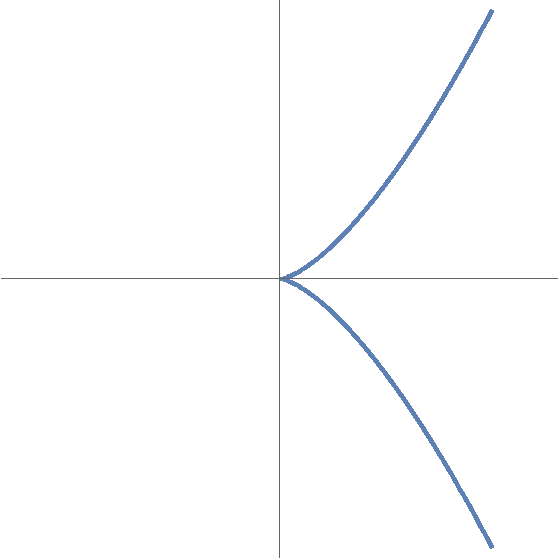
\includegraphics[scale=0.5]{Y^2-X^3}
\end{center}

$$
\left\{ \begin{aligned}
f&=Y^2-X^3\\
\frac{\pd f}{\pd X}&=-3X^2\\
\frac{\pd f}{\pd Y}&=2Y
\end{aligned}\right.
$$
so $X=Y=0$ is the only singular point.

$$Y^2=X^3-X$$
\begin{center}
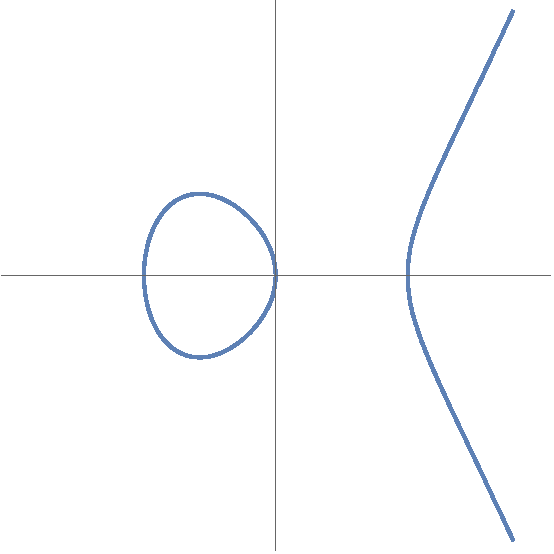
\includegraphics[scale=0.5]{Y^2=X^3-X}
\end{center}
$$
\left\{ \begin{aligned}
f&=Y^2-X^3+X\\
\frac{\pd f}{\pd X}&=-3X^2+1=0\\
\frac{\pd f}{\pd Y}&=2Y=0
\end{aligned}\right.
$$
If $\text{char }k\neq 2$, $\Lrta Y=0$, $X^3-X=0$ $X=0,-1,1$ do not satisfy the system of solutions. In the case $\text{char}=2$, $(1,0)\in Y$ is singular.


The intrinsic characterization was found by Zariski. 
\begin{dfn}
$x\in Y$ variety
\begin{enumerate}[label=(\arabic*)]
\item The \textbf{local ring} of $Y$ at $x$
$$
\begin{aligned}
\calo_{Y,x}&=\{f\in K(Y)|f\text{ defined  at } x\}\\
&=\{\text{ regular functions on some } U\ni x\}/(f_1\sim f_2\text{ if they coincide on } U_{f_1}\cap U_{f_2})
\end{aligned}
$$
if $Y$ is affine, then $\calo_{Y,x}=\{f_1/f_2\in K(Y) \mid f_i\in\calo(Y),f_2(x)\neq 0\}=\calo(Y)_{\scm_x}$, where $\scm_x=\{f\in\calo(Y)|f(x)=0\}$ is the maximal ideal corresponding to $x$.
$$
\calo(Y)\subset\calo_{Y,x}\subset K(Y)
$$
\end{enumerate}
\end{dfn}
\begin{dfn}
$Y\subset \affn^n$ affine $x\in Y$. The (Zariski) cotangent spaces of $Y$ at $x$ is the $K$-vector space
$$
\scm_{Y,x}/\scm_{Y,x}^2,
$$
where $\scm_{Y,x}\subset \calo_{Y,x}$ is the maximal ideal 
\end{dfn}
\begin{rmk}
$\calo_{Y,x}$ is a local ring, it has a unique maximal ideal $\scm$ which is $\scm_x\calo_{Y,x}$ in the affine case. Moreover $\calo_{Y,x}/\scm=K$ by $f\mapsto f(x)$.
\end{rmk}

N.B. Intuitively,  the Taylor expansion of $f\in \calo_{Y,x}$ about $x\in\scm_{Y,x}$ is
$$
f(X)=f(x)+\sum^n_{j=1}\frac{\pd f}{\pd x_j}(x)(X-x_j)+\dots
$$
if $f\in\scm_{Y,x}$ then $f(x)=0$ and terms of order $\geq 2$ belongs to $\scm_{Y,x}^2$, so $f$ has image
$$
\sum \frac{\pd f}{\pd x_j}dX_j\in \scm_{Y,x}/\scm_{Y,x}^2
$$
where $dX_j=X-x_j$.



\begin{dfn}
A local ring $\calo$ with maximal ideal $\scm$ is callled \textbf{regular} if 
$$
\dim \calo= \dim_k \scm/\scm^2
$$
where $k=\calo/\scm$ is the residue field.
\end{dfn}

\subsection{Mar 13th-A: Nonsingular variety continue}
%Recall:
%$x\in Y\subset \affn^n$, $d=\dim(Y)$ affine variety,  and $Y$ is non-singular at $x$ iff 
%$$
%rank\ J_{\underline{f}}(x)=n-d.
%$$
\begin{thm}(Zariski)
	For $x\in Y\subset \affn^n$ the following are equivalent:
	\begin{enumerate}[label=(\arabic*)]
		\item
		$Y$ is non-singular at $x$
		\item $\dim(Y)=\dim_K(\scm_{Y,x}/\scm_{Y,x}^2)$, where $\scm_{Y,x}$ is the maximal ideal in the local ring $\calo_{Y,x}:=\calo(Y)_{\tilde{\scm}_{Y,x}}$ with $\tilde{\scm}_{Y,x}=\{f\in\calo(Y)\mid f(x)=0\}$.
	\end{enumerate}
\end{thm}


\begin{rmk}
	One can show $\dim_K\scm_{Y,x}/\scm_{Y,x}^2\geq \dim (Y)$ so the question is whether it is larger or not. 
\end{rmk}

\begin{proof}
	Denote $I:=I(Y)$, $d= \dim Y$ and  $x:=(x_1,...,x_n)\in\affn^n$.
	Let $I_x:=(X_1-x_1,...,X_n-x_n)\subset \calo(\affn^n)$ so that $\tilde{\scm}_{Y,x}=I_x/I$.
	There  is an isomorphism of $K$-vector spaces
	$$
	\theta:\left\{\begin{aligned}
	I_x/I_x^2&\lrta K^n\\
	f&\longmapsto \left(\frac{\pd f}{\pd X_j}(x)\right)_{1\leq j\leq n}
	\end{aligned}\right. .
	$$
	To see this, note that $f\in I^2_x$ iff $f=\sum_{i,j}h_{ij}(X_i-x_i)(X_j-x_j)$ and thus each $f \in I_x/I_x^2$ can be expressed as
	$$
	f=\sum_{i}^n(X_i-x_i)\frac{\pd f}{\pd X_i}(x)+I_x^2.
	$$
	That means each $f$ is uniquely defined by its derivatives and this preserves scalar multiplication.
	
	Let $(f_1,...,f_m)$ be a generating set of $I$. Then $(\theta(f_1),...,\theta(f_m))$ are the columns of $J_{\underline{f}}(x)$ and for any $f\in I$ we can write
	$$
	f=\sum_j g_j f_j
	$$
	for some $g_j \in K[X]$. Thus
	$$
	\frac{\pd f}{\pd X_i}(x)=\sum^n_{j=1} g_j(x)\frac{\pd f_j}{\pd X_i}(x).
	$$
	In vector notation this is
	$$
	\theta(f)_i=\sum^n_{j=1} g_j(x) \theta(f_j)_i .
	$$
	We conclude that the span of the $\theta(f_j)$ is $\theta((I+I_x^2)/I_x^2)$, so 
	$$
	rank\  J_{\underline{f}}(x)=\dim_K\theta((I+I_x^2)/I_x^2) = \dim_K (I+I_x^2)/I_x^2 .
	$$
	Consider the short exact sequence
	$$
	0 \lrta (I +I_x^2)/I_x^2  \lrta I_x/I_x^2 \lrta I_x/(I+I_x^2)  \lrta 0 .
	$$
	From this we see that 
	$$ rank \ J_{\underline{f}}(x) + \dim_K  I_x/(I+I_x^2) = \dim_K I_x/I_x^2 .$$  
	We already established that the RHS is $n$ hence $x$ is non-singular iff 
	$d=\dim_K I_x/(I+I_x^2)$. 
	
	Consider 
	$$
	\begin{tikzcd}
	I_x \arrow[r] \arrow[rr, "\varphi"', bend right] & \tilde{\scm}_{Y,x}\subset \scm_{Y,x} \arrow[r] & \scm_{Y,x}/\scm_{Y,x}^2
	\end{tikzcd}
	$$
	Note $\varphi(I+I_x^2)=0$ so we get a $K$-linear map 
	$$
	I_x/(I+I_x^2)\lrta \scm_{Y,x}/\scm_{Y,x}^2
	$$
	\underline{Claim}: This is an isomorphism $[\Lrta$ the theorem].  
	(a) $\varphi$ is surjective: 
	$h\in \scm_{Y,x}\subset \calo_{Y,x}\subset K(Y)$, $\Lrta h=\frac{h_1}{h_2}$, with $h_1, h_2\in\calo(Y)$ and $h_2(x)\neq 0, h_1(x)=0$. Then $$
	h-\frac{h_1}{h_2(x)}=h_1\left(\frac{h_2(x)-h_2}{h_2(x)h_2}\right)\in\scm_{Y,x}^2$$
	$$
	\Lrta [h]=\varphi\left(\frac{h_1}{h_2(x)}\right),
	$$
	where $\frac{h_1}{h_2(x)}\in I_x$, so $\varphi$ is surjective.
	
	(b) $\ker(\varphi)=I+I_x^2\subset I_x$ (Intuitively, the restriction of $f$ on $Y$ vanishes to order $2$ ar $x$). 
	
	\underline{Precisely}: 
	$$
	\calo_{Y,x}=(\calo(\affn^n)/I)_{I_x/I}=\calo(\affn^n)_{I_x}/I\calo(\affn^n)_{I_x}
	$$
	the last equality from commutative algebra. $\varphi(f)=0$ means that $f\mod I$ belongs to $(I_x^2)_{I_x}$ which is an ideal in $\calo(\affn^n)_{I_x}$ generated by $I_x^2$
	$$
	f\mod I=\sum_{i,j}(X_i-x_i)(X_j-x_j)h_{ij}
	$$
	$\theta(f\mod I)=0\Lrta f\in I+I_x^2$.
\end{proof}

\begin{thm}
Let $Y\subset \affn^n$ affine variety. Then $Y^\circ =\{x\in Y\mid Y\text{ non-singular at } x\}$  is dense open subset.
\end{thm}
\begin{cor}
Any variety $Y$ is birational to a non-singular variety.
\end{cor}
\begin{proof}
(of theorem)\\
Let $S=Y-Y^\circ=\{\text{ singular points }\}$. Then we know

$(1)$ $S$ is closed in $Y$, indeed fixing $(f_1,...,f_m)$ generating $I(Y)$
$$
S=\{x\mid rank\  J_{\underline{f}}(x)\neq n-d\} 
$$
One can show that $rank\ J_{\underline{f}}(x)\leq n-d$. So
$$
\begin{aligned}
S&=\{x\mid rank\  J_{\underline{f}}(x)< n-d\}\\
&=\{x\in Y\mid \text{ for all minors $M$ of $J_{\underline{f}}$ of size $n-d$ are degenerate $\det (M)=0$.}\}
\end{aligned}
$$
is a closed algebraic set in $\affn^n$.

$(b)$, $S\neq Y(\Lrta Y^\circ\neq \emptyset$ and open, so is dense). 

If $S=Y$, then by the theorem of Zariski, the set of non-singular points in an open set of a hypersurface birational to $Y$ would be empty. This means that we may assume $Y=V(f)\subset \affn^{d+1}$ with $f$ non-zero irreducible.
 Then 
 $$
V(f)\supset S=\left\{x\in \affn^{d+1}|0=f(x=\frac{\pd f}{x_1}(x)=...=\frac{\pd f}{x_d}(x)\right\}
 $$
 so if $S=V(f)$, $\frac{\pd f}{\pd x_1}\in I(V(f))=f\calo(\affn^{d+1})=f K[X_1,..,X_{d+1}]$

 $\Lrta$If char $0$, comparing degrees, we have contradiction.

 $\Lrta$If char $=p\neq 0$, we get $\frac{\pd f}{\pd x_i}=0$ for $1\leq i\leq d$,
 $\Lrta f\in K[X_1^p,..,X_d^{p}]\Lrta f=g^p$ because  $\text{char }K=0$ , and this is contradicting the irreducibility.
\end{proof}
\section{Schemes}
In this chapter we will mainly follow chap 2 of Hartshorne and chap 1 of Eisenbud-Harris.
\subsection{Mar 13th-B: Affine schemes}
\subsubsection{Motivations}
Serious problems with classical approach occurred in late 1950's
\begin{enumerate}[label=(\arabic*)]
\item Intrinsic definitions (Without embeddings into $\affn^n$ or $\proj^n$)
\item Construction of various algebraic varieties especially Jacobian variety of a curve, especially w.r.t. base field (is the Jacobian of a curve given by equation with coefficients in the same field?)
\item Reduction modulo $p$ of a variety given by equation in $\intg[X_1,..,X_n]$
\end{enumerate}
To attack $(1)$, Serre started from
$$
\begin{aligned}
\left\{\text{alg. set }Y\subset \affn^n \right\}&\llrta \left\{\text{fin.gen. reduced $K$-algebra}\right\}\\
Y&\mapsto \calo(Y)\\
\{\text{maximal ideals in $A$}\}&\mapsfrom A.
\end{aligned}
$$

Grothendieck tried to remove the restriction on the algebras and managed to interpret it geometrically.
$$
\begin{aligned}
\left\{\text{affine schemes }\right\}&\llrta \left\{\text{all commutative rings.}\right\}\\
\end{aligned}
$$

To each ring $A$, we will associate a geometric object called its \textbf{spectrum} denoted $\spec(A)$.

(1) $\spec A$ is a set. 
$\spec A\neq \{\text{ maximal ideals }\}$ because this choice is not functorial. If $A_1\overset{f}{\lrta} A_2$, we want $\spec(A_2)\overset{f^*}{\lrta}\spec(A_1)$ which would have to be $f^*(\scm)=f^{-1}(\scm)\subset A_1$. But $f^{-1}(\scm)$ is \underline{NOT} necessarily maximal.
\begin{ex}
$A$ is an integral domain
$$
\{0\}\subset A\inj Frac(A)\supset\{0\}\text{ maximal }
$$
\end{ex}
\begin{dfn}
$\spec A:=\{\text{ prime ideals $\scp\subset A$ }\}$
\end{dfn}

\underline{Fact}: If $f: A_1\lrta A_2$ is a ring morphism then $\scp\mapsto f^{*}\scp$ gives map of sets
$$
\spec A_2\lrta \spec A_1
$$
\begin{proof}
$$A_1\overset{f}{\lrta}A_2/\scp$$
$$f^{-1}\scp\mapsto 0$$
 leads to an injective map
 $$
A_1/f^{*}\scp\inj A_2/\scp,
$$ then $A/f^{-1}\scp$ is an integral domain and $f^*(\scp)$ is therefore a prime ideal.
\end{proof}

\begin{dfn}
If $\scp\in\spec A$. the fraction field of $A/\scp$ is called the \textbf{residue field} at $\scp$, denoted $\kappa(\scp)$. 
\end{dfn}
If $a\in A$, then $a$ defines a function
$\tilde{a}:\spec A\lrta\coprod_{\scp\in \spec(A)}\kappa(\scp)$, $\scp\mapsto a\mod \scp$


\subsubsection{$\spec A$ as a topological space}
\begin{dfn}
For any set $S\subset A$, let $V(S)=\{\scp\in\spec(A)|S\subset \scp\}$, the set of point $\scp$ where each element in $S$ vanishes.
\end{dfn}
\underline{Note}: 
\begin{enumerate}[label=(\arabic*)]
\item $V(S)=V(\text{ ideals generated by $S$ })$
\item Not always true that $V(S)=V(\text{ finitely many elements})$
\item $V(S)=\{\scp\in\spec A|\forall x\in S, \tilde{x}(\scp)=0\in\kappa(\scp)\}$
\end{enumerate}

\begin{lemma}\ 
\begin{enumerate}[label=(\arabic*)]
\item The sets $V(I)$, $I$ ideal in $A$, from  the closed sets of a topology on $\spec A$ (called the \textbf{Zariski topology}).
\item $V(I)\subset V(J)\Llrta \sqrt{J}\subset \sqrt{I}$
\item If $f: A_1\lrta A_2$ is a ring morphism, then 
$$
f^*:\spec(A_2)\lrta \spec(A_1)
$$
is continuous.
\end{enumerate}
\end{lemma}
\begin{proof}
(1) $\emptyset =V(A)=V(\{1\})$ $\spec A=V(\{0\})$.
$$
\begin{aligned}
\cap_{i\in X}V(I_i)&=\{\scp\in \spec(A)|I_i\subset \scp\text{ for every $i$}\}\\
&=\{\scp\in \spec(A)|\sum I_i\subset \scp\}\\
&= V\left(\sum_{i\in X}I_i\right)
\end{aligned}
$$
$$
\begin{aligned}
V(I)\cup V(J)&=\{\scp\in\spec (A)|I\subset \scp\text{  or } J\subset \scp\}\\
&=\{\scp\in\spec A|I J\subset \scp\}(\text{because $\scp$ prime})\\
&=V(IJ)
\end{aligned}
$$

(2) recall the definition of radicals of an ideal 
$$
\begin{aligned}
\sqrt{I}&:=\{x\in A|\exists k\geq 0, x^k\in I\}
&=\cap_{I\subset \scp,\scp\in\spec A}\scp\\
&=\cap_{\scp \in V(I)}\scp
\end{aligned}
$$
then if $V(J)\subset V(I)$, we get $\sqrt{I}\subset \sqrt{J}$.

Conversely, if $\sqrt{I}\subset \sqrt{J}$ then for $\scp\in V(J)$, then
$I\subset \sqrt{I}\subset\sqrt{J}\subset \scp\Lrta \scp\in V(I)$.

(3) Assume $S$ is a subset in $B$. Consider a closed set $V(S)$ in $\spec B$, we will verify that $\pi^{-1}V(S)$ is also closed.
$$
\pi^{-1}V(S)=\{[\scp]\in \spec A: \pi(\scp)\supset S\}=\{[\scp]\in \spec A: \phi^*(\scp)\supset S\}
$$
\underline{Claim}: $\pi^{-1}V(S)=V(\phi(S))$

In fact $\scp\supset \phi(S)\Llrta \phi^{-1}(\scp)\supset S$, therefore,
$$
\pi^{-1}V(S)=\{[\scp]\in \spec A: \phi^*(\scp)\supset S\}=\{[\scp]\in \spec A: \scp\supset \phi(S)\}=V(\phi(S)).
$$
The preimage of a closed set is always closed. $\pi$ is continuous.
\end{proof}

\subsection{Mar 16th: Affine schemes, examples and properties.}
Recall

$A$ is a ring with unity
$\spec A=\{\text{ prime ideals in $A$}\}$

closed sets: for a subset $S\subset A$,
$V(S)=V(I:=\text{ ideal generated by $S$})$ $=\{\scp|I\subset \scp\}$

If $A\overset{f}{\lrta} B$ is a ring morphism, then $f^*:\spec(B)\lrta \spec (A)$: $\scp\mapsto f^{-1}(\scp)$ is continuous.

Indeed, let $V(I)\subset \spec A$ be closed,, then $(f^{*})^{-1}(V(I))=\{\scp\in\spec (B)|f^*(\scp)\in V(I)\}=\{\scp\in\spec B|I\subset f^{-1}\scp\}=\{\scp \in \spec B\mid f(I)\subset \scp\}$, therefore
$$
(f^{*})^{-1}V_A(I)=V_B(f(I))
$$

\subsubsection{Examples of $\spec A$}
\begin{ex}
$\spec (\{0\})=\emptyset$

By definition, this is the only ring with $\spec A$ empty.
\end{ex}

\begin{ex}\label{ex:K-algebra}
$K$ algebraically closed field, $\emptyset\neq Y\subset K^n$ affine algebraic set. The corresponding  affine scheme is 
$$
Y^{sc}
=\spec (\calo(Y))$$
in other words
$$
Y^{sc}=\spec (K[X_1,...,X_n]/I(Y)=:A).
$$
Maximal ideals of $\calo(Y)$ are in bijection with points of $Y$ by 
$$
x\mapsto \scm_x=\{f\in\calo(Y)|f(x)=0\}
$$
so we get an injective map
$$
Y\overset{\varphi}{\lrta} Y^{sc}
$$
$$
x\longmapsto \scm_x
$$
This map $\varphi$ is continuous, when both $Y$ and $Y^{sc}$ are endowed with Zariski topologies.

Let $V(I)\subset Y^{sc}$ be closed and $I\subset \calo(Y)$.
$$
\begin{aligned}
&\varphi^{-1}(V(I))\\
&=\{x\in Y\mid \scm_x\in V(I)\}\\
&=\{x\in Y\mid I\subset\scm_x\}\\
&=\{x\in Y\mid \forall f\in I, f(x)=0\}
\end{aligned}
$$
is a closed algebraic set in $K^n$.

Observe: for every $x\in Y$, the residue field of $\scm_x$ is $A/\scm_x \cong K$ where the function associated to $f\in A$ is given by 
$$
\tilde{f}(\scm_x)=f(x).
$$

The following are equivalent
\begin{enumerate}
\item $Y\overset{\varphi}{\lrta} Y^{sc}$ is surjective
\item every prime ideal in $\calo(Y)$ is maximal
\item $\dim \calo(Y) = 0$.
\end{enumerate}
Consider the case $Y=K$ and $Y^{sc}=\spec (K[X])$ with $\dim Y=1$.
$K[X]$ is a principal ideal domain and $K$ is algebraically closed.
$$
Y^{sc}=\{(X-x)|x\in K\}\cup \{0\}
$$
where $\eta:=\{0\}$ is called the generic point of $Y^{sc}$.

\underline{Claim}: $\{\eta\}$ is not closed in $Y^{sc}$, in fact it is dense
$$
\overline{\{\eta\}}=Y^{sc}.
$$
\end{ex}

\begin{ex}
More generally, Let $A$ be an integral domain and $\eta=\eta_A=\{0\}\in\spec A$.

\underline{Claim}: 
$$
\overline{\{\eta\}}=\spec A
$$

Let $\scp\in\spec A$.
$$
\begin{aligned}
\overline{\{\scp\}}&=\bigcap_{\scp\in V(I)}V(I)\\
&=\bigcap_{I\subset \scp}V(I)\\
&=V(\sum_{I\subset\scp} I )=V(\scp)
\end{aligned}
$$
$$
\overline{\{\scp\}}=V(\scp)=\{Q\in\spec(A)|\scp\in Q\}
$$
So:
\begin{enumerate}
\item $\overline{\{\eta_A\}}=\spec A$ if $A$ is an integral domain.
\item $\{\scp\}$ is closed iff $\scp$ is maximal.
\end{enumerate}
There is a one to one correspondence between prime ideals in $A$ and irreducible closed subsets in $\spec A$.
\end{ex}

\begin{dfn}
If $\scp\in\overline{\{Q\}}$, we say that $\scp$ is a \textbf{specialization} of $Q$, and that $Q$ \textbf{specializes to} $\scp$. In the case of affine scheme $\scp\in \overline{\scq}$ iff $\scp\in V(\scq)\Llrta \scp\supset \scq$.
\end{dfn}

\begin{ex}
Any point is a specialization of $\eta_A$ if $A$ is integral domain. What is $\kappa(\eta_A)$?
$$
A/\{0\}=A
$$
so $\kappa(\eta_A)=Frac(A)$.
\end{ex}

Back to the Example \ref{ex:K-algebra}

$Y=K$, $Y^{sc}=\spec (K[X])$, $\eta=\{0\}$ is dense in $Y^{sc}$, its residue field is $K(X)$.

\begin{rmk}
If $f_1,f_2\in K[X]$ are such that they coincide at $\eta$;
$$
\tilde{f}_1(\eta)=\tilde{f}_2(\eta)
$$
then in fact $  f_1=f_2$ in $K[X]$.
\end{rmk}

We will often encounter situations like ``A property holds at $\eta$ $\Lrta$ it holds at for all $x$ in an open set''

\begin{ex}
$A$ is an integral domain. Any $\emptyset \neq U$ open set in $\spec A$ is dense:
$$
U\cap \{\eta\}\neq \emptyset
$$
so $\eta\in U$, $\Lrta \overline{\{\eta\}}=\overline{U}$
\end{ex}

\begin{ex}
The Zariski topology is \textbf{quasi-compact}: any open covering has a finite subcover. Indeed, suppose
$$
\begin{aligned}
&\bigcap_\alpha V(I_\alpha)=\emptyset\\
\Llrta & V(\sum_\alpha I_\alpha)=\emptyset=V(A)\\
\Llrta & 1\in \sum_\alpha I_\alpha\\
\Llrta & 1=\sum_{j=1}^{m} f_{\alpha_j}, f_{\alpha_j}\in I_{\alpha_j}\\
\Llrta & V(\sum_j I_{\alpha_j})=\emptyset\\
\Llrta & \bigcap_j V(I_{\alpha_j})=\emptyset
\end{aligned}
$$
\end{ex}
\begin{ex}
For any $I\subset A$, $A\overset{\pi}{\lrta} A/I$ induces 
$$
\spec (A/I)\overset{\pi^*}{\lrta}\spec A
$$
which  gives homeomorphism 
$$
\spec (A/I)\cong V(I).
$$
\end{ex}

\begin{ex}
$K$ is a field, not necessarily algebraically closed. Let $J\subset K[X_1,..,X_n]$ be an ideal and $Y=\spec (K[X_1,...,X_n]/J)$. (Want to understand in particular the relation with the case $K$ is algebraically closed.) Fix $L \supset K$  where $L$  is algebraically closed Then we get an injective ring morphism 
$$
K[X]/J\lrta L[X]/JL[X]
$$
hence a map
$$
Y_L:=\spec(L[X]/JL[X])\lrta Y,
$$
where $\spec(L[X]/JL[X])$ is a classical algebraic set (if $J$ is prime).

Take
$Y=\spec (K{X})=\affn^1_K$.

\begin{dfn}
	Let $A$ be any ring. The \textbf{affine $n$-space} $\affn^n_A$ over $A$ is $\spec A[X_1,...,X_n]$.
\end{dfn}
	
	


What is $\affn^1_L\lrta \affn^1_K$? (induced by $K[X]\lrta L[X]$)
$$
\begin{aligned}
\affn^1_K&=\{\scp\subset K[X]\text{ prime}\}\\
&=\{0\} \cup \{fK[X]\mid f \text{ irreducible and monic}\}
\end{aligned}
$$
\underline{Check}: the Zariski topology has  closed sets $\emptyset$, $\affn^1_K$, finite sets of closed points. Given $i: K[X]\inj L[X]$, what is 
$\affn^1_L\overset{i^*}{\lrta }\affn^1_K$? We have that
$$
\begin{aligned}
i^*(\eta_L)&=i^{-1}(\{0\})\\
&= \eta_K
\end{aligned}
$$
which means the image of $i^*$ us dense.

Let $x\in L$
$$\begin{aligned}
&i^*(X-x)L[X]\\
&=i^{-1}((X-x)L[X])\\
&=\{f\in K[X]\mid (X-x)|f\text{ in } L[X]\}\\
&=\{f\in K[X]\mid f(x)=0\}
\end{aligned}
$$
\underline{Case 1}: $x$ is transcendental over $K$ 
$$
\Llrta i^*(x)=\{0\}=\eta_K
$$
\underline{Case 2}: $x$ is algebraic over $K$
$$
i^*(x)=f_x
$$
 where $f_x$ is the minimal polynomial $x$ over $K$.

 Observe that $i^*$ is not injective more precisely,
 $$
(i^*)^{-1}(f)=\{\text{ roots of $f$ in $L$}\}
 $$
 where $f$ is irreducible monic.
\end{ex}

\begin{ex}
Given $A,B$ integral domain 
$A\overset{f}{\lrta} B$ is injective iff
$$
f^{*}(\spec B)\subset \spec A
$$ is  dense. The proof is left as an exercise.


If $A\overset{f}{\lrta} B$ is injective,  we have $f^{*}(\eta_B)=\eta_A$, it maps the generic point to the generic point, therefore the image is dense because $f^*(\spec B)\ni \eta_A$. 

Conversely, if $f^{*}(\spec B)$ is dense in $\spec A$, we know $f^{*}(\eta_B)$ is dense in $\spec A$ and the only possibility is that it maps the generic point to the generic point, which means the ring morphism is injective.
\end{ex}

\begin{ex}
$K=\overline{K}$, 

$Y^{sc}$ for $Y=\{(x,y)\in K^2 \mid (xy)=0\}$. ($Y$ is not a variety in this case but only an algebraic set.)
$$
\affn^2_K\supset V(xy)\cong Y^{sc}=\spec(K[X,Y]/(XY))
$$
Check the points of $Y^{sc}$ are
\begin{align*}
h_x & = \lgl (X-x), Y\rgl\subset K[X,Y]/(XY) \\
v_y & =\lgl X, (Y-y)\rgl
\end{align*}
because $XY=(X-x)Y+xY$.
$h_x$ and $v_y$ are closed points with residue field $K$.  Let
\begin{align*}
\eta_1 & =X K[X,Y]/(XY) \\
\eta_2 & =YK[X,Y]/(XY).
\end{align*}
We have $\{0\}\notin \spec (K[X,Y]/(XY))$ because the ring is not an integral domain.
$$
\begin{aligned}
\overline{\{\eta_1\}}&=\{\eta_1\}\cup \{\scm \text{ maximal s.t. } X\subset \scm\}\\
&=\{\eta_1\}\cup \{v_y \mid y\in K\}.
\end{aligned}
$$
Similarly, we have
$$
\overline{\{\eta_2\}}=\{\eta_2\}\cup\{h_x \mid x\in K\}.
$$
Note $v_0=h_0$ is a specialization of both $\eta_1$ and $\eta_2$.
\end{ex}

\begin{ex}
For  $K=\overline{K}$ consider
 $$\affn^2_K=\{(x, y) \mid (x,y)\in K^2\} \cup \{\eta\}\cup \{fK[X,Y] \mid f \text{ irreducible monic}\}$$ 
 where we identify the maximal ideals $(X-x, Y-y)$ in $K[X,Y]$ with points $(x,y)$. 
Note that prime ideals of height $1$ are principal in a UFD.
$$
\overline{\{fK[X,Y]\}}=\{f K[X,Y]\}\cup \{(x,y)\in K^2|f(x,y)=0\}
$$
For this reason, we denote $\{fK[X,Y]\}$ by $\eta_f$ because it is the generic point of $V(f)$.
\begin{align*}
\overline{\{\eta_f\}} & =\eta_f\cup \text{ classical points on } C_f \\
\kappa(\eta_f) & =K[X,Y]/fK[X,Y]=\kappa(C_f) 
\end{align*}
where $C_f$ is the classical curve.
$\eta_f$ specializes to the point $(x,y)$ on $C_f$.

\end{ex}

\subsection{Mar 20th: Structure sheaf over affine scheme}

\begin{ex}
$A=\intg$, $\spec A=\{0\}\cup \{p\intg|p\text{ prime number}\}$.
Recall $\dim (\intg)=1$, with residue fields 
$$
\left\{\begin{aligned}
&K(\eta)=\ratl\\
&K(p\intg)=\intg/p\intg=\bbf_p, \text{  finite field }
\end{aligned}\right.
$$
A statement like `` property  $P$ is true at $\eta$'' $\Lrta $`` It is true on any open set'' means ``a property $P$ true for $\ratl$ is also true for $\mod p$ for $p$ large enough.''

(Topology has closed sets $\emptyset, \spec \intg, V(n\intg)=\{p\intg: p\textbf{ divides }n\}$, where $V(n\intg)$ is a finite set of closed points.)

$$
\intg\lrta \bbf_p\llrta \begin{aligned}
&\spec (\bbf_p)\inj \spec (\intg)\\
& \{0\}\in\bbf_p\mapsto  p\intg
\end{aligned}
$$
$$
\intg\overset{i}{\inj} \ratl\llrta \begin{aligned}
&\spec (\ratl)\overset{i^*}{\lrta} \spec (\intg)\\
& \{0\}\in\ratl\mapsto  \eta
\end{aligned}.
$$
In particular, the image of $i^*$ is dense in $\spec \intg$.
\end{ex}
\section*{structure sheaf}

Note recall we want
$$
\{\text{affine schemes}\}\llrta \{\text{ commutative rings}\}
$$
$$
\spec A\mapsfrom A
$$
$$
f^*\mapsfrom f
$$
This is functorial but cannot capture the whole category of rings because for instance all rings
$$
A=K[X]/(X^n), n\geq 1
$$
($K$ is a field). We have $\spec A=\{XK[X]\}$, independent of $K$ and $n$. We need to remember what is $K$ and  what is $n$.

We deal with this non-reduced ``fuzz'' by defining ``regular functions''
\begin{dfn}
$A$ is a ring. For $U\subset \spec A$ open, we define the ring $\calo(U)$ of ``regular functions on $U$'' by 
$$
\calo(U)=
\left\{s:U\lrta \bigsqcup_{\scp\in U}A_\scp\left| \begin{aligned}
& \text{(1) $s(\scp)\in A_\scp$ for $\scp \in U$}\\
&\text{(2)} \forall \scp\in U, \exists V \text{ open  nbhd of } \scp \text{ in } U\\
& \text{ and } a\in A, f\in A,\\
& \text{ s.t.} \forall \scq\in V, f\notin \scq \text{ and } s(\scq)=a/f\in A_\scq\\
\end{aligned}\right\}
\right.
$$
\end{dfn}
Note: if $V\subset U$ open then $s\mapsto s|_V$ is a ring morphism $res^U_V:\calo(U)\lrta \calo(V)$ and $res^U_V=id_{\calo(U)}$. Then the pair $\left((\calo(U))_{U\in\spec A}, (res^U_V)_{U,V\in \spec A}\right)$ is a \textbf{ sheaf of rings } on $\spec A$. 
\begin{dfn}
$X$ is a topological space, $\calc$ a category,
\begin{enumerate}[label=(\arabic*)]
\item A \textbf{$\calc$-presheaf} is sthe data of 
\begin{enumerate}[label=(\alph*)]
\item For every open set $U\subset X$, an object $\calf(U)=\Gamma(U,\calf)$ in $\calc$.
\item For every $V\subset U$ opens in $X$, a $\calc$-morphism $res^U_V: \calf(U)\lrta \calf(V)$
\end{enumerate}
such that given $U$ opens in $X$.
\begin{enumerate}[label=(\roman*)]
\item $res^U_U=id_{\calf(U)}$
\item Given $W\subset V\subset \subset U$ opens in $X$
$$
res^U_W=res^V_W\circ res^U_V
$$
\underline{Notation:} $res^U_V(s)=s|_V$
\end{enumerate}

\item A $\calc$-presheaf is a \textbf{$\calc$-sheaf} if: for any $U\subset X$ open, for every open covering $U=\cup_\alpha V_\alpha$, for any family $(s_\alpha)_\alpha$ with $s_\alpha\in \calf(V_\alpha)$ such that $s_\alpha|_{V_\alpha\cap V_\beta}=s_{\beta}|_{V_\alpha\cap V_\beta}$, there is a unique $s\in \calf(U)$ with $s|_{V_\alpha}=s_\alpha$.
\end{enumerate}
\end{dfn}
\begin{exercise}
Check that the sheaf of regular functions is indeed a sheaf.
\end{exercise}
\begin{dfn}
$A$ a ring. The \textbf{affine scheme} associated to $A$ is $(\spec A,\calo)$ where the first data is endowed with Zariski's topology and the $\calo$ is the structure sheaf.
\end{dfn}

\begin{ex}
$K$ a field, $\spec K=\{\eta\}$
$$
\left\{
\begin{aligned}
&\calo(\spec K)=\{s:\eta\lrta K_{\{0\}}=K,\ (\text{ i.e. } s(\eta)\in K)\} \\
&\calo(\emptyset)=\{0\}
\end{aligned}
\right.
$$
Different K gives different affine schemes.
\end{ex}

\begin{prop}
For $f\in A$, define $U_f=\{\scp\in \spec A|f\notin \scp\}$
\begin{enumerate}[label=(\arabic*)]
	\item $U_f$ is a open ``basic open sets''
	\item We have a canonical isomorphism
	$$
	\left\{
	\begin{aligned}
	& A_f\overset{\psi}{\lrta}\calo(U_f)\\
	& a/f^m\longmapsto (s:\scp\in U_f\mapsto \frac{a}{f^m}\in A_\scp)
	\end{aligned}
	\right.
	$$
\end{enumerate}
In particular, for $f=1$, we get a canonical isomorphism
$$
A=A_1\overset{\sim}{\lrta}\Gamma(\spec A,\calo)
$$
$\Lrta$ the affine scheme of $A$ allows you to recover $A$.
\end{prop}
\begin{proof}
(injectivity)

Suppose $\psi\left(\frac{a}{f^m}\right)=0$. This means that 
$$
\forall \scp\in U_f, \frac{a}{f^m}=\frac{0}{1}\in A_\scp
$$
$\Llrta \forall \scp\in U_f$, $\exists h_\scp\notin \scp,$ $ha=0$. Let $I=\{x\in A|xa=0\}$. $I$ is an ideal and $I\notsubset \scp$ for any $\scp \in U_f$

$\Lrta V(I)\cap U_f=\emptyset$

$\Lrta V(I)\subset V(f)$

$\sqrt{(f)}\subset \sqrt{I}$

$f\in \sqrt{(f)}\in\sqrt{I}$

$\exists k\geq 0, f^ka=0\Lrta a/f^m=0\in A_f$

(Surjectivity): We need the following lemma
\begin{lemma}\ 
\begin{enumerate}[label=(\arabic*)]
\item $U_{f_1}\cap U_{f_2}=U_{f_1f_2}$
\item $U_{f^n}=U_{f}, V(f^n)=V(f)$
\item $U_f$ is quasicompact
\item The open sets $U_f$ forms a basis of the Zariski topology.
\end{enumerate}
\end{lemma}
Consider $\psi:A_f\lrta \calo(U_f)$, let $s\in \calo(U_f)$.

By definition there exists an open covering of $U_f$, $U_f=\bigcup_\alpha V_\alpha$, and elements $a_\alpha, g_\alpha$ such that $\forall \scp\in V_\alpha$, $s(\scp)=\frac{a_\alpha}{g_\alpha}, g_\alpha\notin \scp$.

Using the above lemma,  we may assume  there are finitely many $V_\alpha$ and $V_\alpha=U_{h_\alpha}$.

\underline{Observe}: $\forall \scp\in U_{h_\alpha}=V_\alpha$, $g_\alpha\notin\scp\Llrta \scp\in U_{g_\alpha}$
$$
\begin{aligned}
&U_{h_\alpha}\subset V_{g_\alpha}\\
& \Lrta V(g_\alpha)\subset V(h_\alpha)\\
&\Lrta \sqrt{(h_\alpha)}\subset \sqrt{(g_\alpha)}\\
&\Lrta \exists n_\alpha, h^{n_\alpha}_{\alpha}\in (g_{\alpha})
\end{aligned}
$$
So $h^{n_\alpha}_\alpha=c_\alpha g_\alpha$, Now for $\scp\in U_{h_\alpha}$
$$
\frac{a_\alpha}{g_\alpha}=\frac{a_\alpha c_\alpha }{g_\alpha c_\alpha}=\frac{a_\alpha c_\alpha}{h_\alpha^{n_\alpha}}\in A_\scp
$$
Replacing $a_\alpha$ by $a_\alpha c_\alpha$, $g_\alpha$ by $h^{n_\alpha}_{\alpha}$, Using $U_{h_\alpha^{n_\alpha}}=U_{h_\alpha}$, we reduce to the case where $g_\alpha=h_\alpha$ for all $\alpha$.

By $U_{h_\alpha}\cap U_{h_\beta}=U_{h_\alpha h_\beta}$, we have
$$
\forall \scp \in U_{h_\alpha h_\beta}, \frac{a_\alpha}{h_\alpha}=\frac{a_\beta}{h_\beta}\text{  in } A_\scp
$$
$$
\Lrta \exists n(\alpha, \beta), (h_\alpha h_\beta)^{n(\alpha, \beta)}(a_\alpha h_\beta-h_\alpha a_\beta)=0
$$

Take $n$ to be the largest of the finite many $n(\alpha,\beta)$
$$
\Lrta(h_\alpha h_\beta)^{n}(a_\alpha h_\beta-h_\alpha a_\beta)=0
$$
$$
a_\alpha' h'_\beta-a_\beta' h_\alpha'=0
$$
where $a_\alpha'=a_\alpha h_\alpha^n$ and $h'_\alpha=h_{\alpha}^{n+1}$

Note 
$\frac{a_\alpha'}{h_\alpha'}=\frac{a_\alpha}{h_\alpha}$ in $A_\scp$ for all $\scp\in U_{h_\alpha'}=U_{h_\alpha}$.

Now
$$
\begin{aligned}
& \bigcup_\alpha U_{h_\alpha'}=U_f\\
& V(f)=V(\sum (h'_\alpha))\\
&\Lrta \sqrt{f}=\sqrt{\sum(h_\alpha')}\\
& \Lrta f^k =\sum_\alpha h_\alpha' c_\alpha\ \text{ for some } k
\end{aligned}
$$
Define 
$$
a=\sum_\alpha c_\alpha a_\alpha'\in A
$$
Fix $\beta$,
$$
a h_\beta'=\sum_\alpha c_\alpha a_\alpha' h'_\alpha=\sum_\alpha c_\alpha a_\beta' h'_\alpha
=a_\beta' f^k
$$
$$
\Lrta s(\scp)=\frac{a_\beta}{h_\beta}= \frac{a_\beta'}{h_\beta'}=\frac{a
}{f^k}
$$
in $A_\scp $ for any $\scp \in U_{h_\beta}=V_\beta$.

So $\psi(\frac{a}{f^k})|_{V_\beta}=s|_{V_\beta}$ for any $\beta$.
So $\psi(a/f^k)$ and $s$ are elements of $\calo(U_f)$ with restrictions equal on open sets forming a covering of $U_f$, by the uniqueness condition in the definition of sheaf, it follows that $\psi(a/f^k)=s$.
\end{proof}


\begin{proof}(of the lemma)
\begin{enumerate}[label=(\arabic*)]
\item $U_{f_1}\cap U_{f_2}\overset{?}{=}U_{f_1 f_2}$
$$
\begin{aligned}
V(f_1)\cup V(f_2)&=\{\scp\in \spec A|f_1\in \scp \text{ or } f_2\in\scp \}\\
&=\{\scp\in\spec A|f_1f_2\in \scp\}
\end{aligned}
$$
\item $f^n\in \scp \Llrta f\in\scp, n\geq1$
\item Suppose $V(f)\subset \cap_\alpha V(I_\alpha)\Lrta V(\sum I_\alpha)\supset V(f)\Lrta \sqrt{(f)}\subset \sqrt{\sum I_\alpha}$
\end{enumerate}
\end{proof}

\subsection{Mar 23th: Sheaves and stalks}
\begin{ex}
    \begin{enumerate}[label=(\arabic*)]
        \item 
        Let $X$ be a topological space. Then
        $$
            \underline C(U) = \{ f : U \longrightarrow \mathbb C \text{ continuous}\}
        $$
        for $U\subset X$ open is a sheaf. For $X$ a manifold we also have that
        $$
        \underline C^\infty(U) = \{ f : U \longrightarrow \mathbb C \text{ smooth}\}
        $$
        is a sheaf and lastly for $X$ a complex manifold the following is a sheaf:
        $$
        \mathcal H(U) = \{ f : U \longrightarrow \cplx \text{ holomorphic}\}. 
        $$
        \item
        Let $X= \mathbb C^\times$. Then
        $$
        \calf(U) = \{f: U \longrightarrow \mathbb C \text{ holomorphic and } f= g^2 \text{ for some $g$ holomorphic} \}
        $$
        is a pre-sheaf but not a sheaf. A holomorphic function might have a square root locally but not on all of $U$. For example, we can take $U$ to be an annulus around the origin.
    \end{enumerate}
\end{ex}

\begin{dfn}
    Let $\calf_1, \calf_2$ be $\calc$-pre-sheaves on $X$. A \textbf{morphism} of $\calc$-pre-sheaves $ : \calf_1 \longrightarrow \calf_2$ is a collection of morphisms $\varphi_U: \calf_1(U) \longrightarrow \calf_2(U)$ such that for any $V\subset U$ open we have a commutative square
    $$
    \begin{tikzcd}
    \calf_1(U) \arrow[r, "\varphi_U"] \arrow[d, "res^U_V \text{ for } \calf_1"'] & \calf_2(U) \arrow[d, "res^U_V \text{ for } \calf_1"] \\
    \calf_1(V) \arrow[r, "\varphi_V"] & \calf_2(V)
    \end{tikzcd}
    $$
    A morphism of sheaves we define to be the same as a morphism of pre-sheaves.
\end{dfn}
Note that $\operatorname{Id}_{\calf(U)}: \calf(U) \longrightarrow \calf(U)$ gives a morphism and that composition makes sense, i.e. we have that
$$
(\varphi \circ \psi)_U = \varphi_U \circ \psi_U.
$$ 
Thus we have defined the category of $\calc$-pre-sheaves and sheaves.

\begin{ex}\ 
    \begin{enumerate}[label=(\arabic*)]
        \item 
        If $X$ is a complex manifold, there are morphisms
        $$
        \mathcal H \longrightarrow \underline C^\infty \longrightarrow \underline C
        $$
        \item
        If $X\subset \reals^n$ is a manifold, then
        $$
        \left\{
        \begin{aligned}
        \underline C^\infty (U) & \longrightarrow \underline C^\infty(U) \\
        f & \longmapsto \partial f / \partial x_1
        \end{aligned}
        \right.
        $$
        is a morphism of sheaves from $\underline C^\infty \longrightarrow \underline C^\infty$.
    \end{enumerate}
\end{ex}

\begin{prop}
    Suppose $\calf$ is a $\calc$-pre-sheaf on $X$. Then there is a unique, up to unique isomorphism, morphism $\sigma: \calf\longrightarrow \calf^\sigma$, (the \textbf{``sheafification''} of $\calf$) such that for any morphism of presheaves $\varphi: \calf \longrightarrow \mathcal Y$ there is a unique $\varphi^\sigma$ such that $\varphi = \varphi^\sigma \circ \sigma$. In particular $\hom_{\mathsf{PSh}} (\calf, \mathcal Y) = \hom_{\mathsf{Sh}} (\calf^\sigma, \mathcal Y)$.
    $$
    \begin{tikzcd}
    \calf \arrow[r, "\varphi"] \arrow[d, "\sigma"'] & \mathcal Y  \\
    \calf^\sigma \arrow{ru}[swap]{\varphi^\sigma}
    \end{tikzcd}
    $$
    If $\calf$ is a sheaf then $\sigma$ is an isomorphism.
\end{prop}

$\calf^\sigma$ is called the sheaf associated to $\calf$. In order to prove the statement, we need another definition.

\begin{dfn}
    Suppose $\calf$ is a $\calc$-presheaf on $X$. The \textbf{stalk} of $\calf$ at $x\in X$ is 
        $$
        \calf_x := \{ (U,s) \mid x \in U\subset X \text{ open}, s \in \calf(U)\} / \sim
        $$
        with 
        $$(U_1, s_1) \sim (U_2,s_2) \quad \Longleftrightarrow \quad \exists V\subset U_1 \cap U_2 \text{ s.t. } s_1|_V = s_2|_V \text{ and } x \in V.
        $$
        This is also called the ``germs of sections of $\calf$ at $x$''.
\end{dfn}

\begin{prop}
    Let $A$ be a ring and consider $\calo_A$ on $\spec A$. Then the following morphism is an isomorphism:
    $$
    \varphi
    \left\{
    \begin{aligned}
    \calo_{A,\scp} & \longrightarrow A_\scp \\
    (U,s) & \longmapsto s(\scp)
    \end{aligned}
    \right.
    $$
\end{prop}

\begin{proof}
    It follows easily from the definitions that $\varphi$ is well defined. For surjectivity, let $a/f\in A_\scp$, $f\notin \scp$.  Then we can construct $s$ defined on $U_f$ such that $s(\scq) = a/f$ in $A_\scq$ for all $\scq \in U_f$.    
    Next, suppose that $s(\scp)=0$ for some section $(U,s)$. Then we can write $s(\scq) = a/f$ for any $\scq\in V$ where $V$ is an open neighbourhood of $\scp$ in $U$. Since $s(p)=0$, we get $ha=0$ for some $h \notin p$. But then on $V \cap U_h$, $s\equiv 0$. 
\end{proof}

Now we get back to the construction of $\calf^\sigma$. Define
$$
\calf^\sigma(U) := \left\{ 
    s: U \longrightarrow \bigsqcup_{x \in U} \calf_x \left| 
    \begin{aligned}
    & \forall x \in U, s(x) \in \calf_x \text{ and} \\
    & \forall x \in U, \exists V \subset U \text{ open, s.t. } x\in V, \\
    & \exists t \in \calf(V) \text{ s.t. } \forall y \in V, s(y) = t_y 
    \end{aligned}
    \right\} \right.
$$
where $t_y$ denotes the equivalence class $[(V,t)]\in \calf_y$.
Moreover, define $\varphi^\sigma: \calf \longrightarrow \calf^\sigma$ by 
$$
\varphi^\sigma_U(t) = (x \longmapsto t_x)
$$
and for $s \in \calf^\sigma(U)$, $V\subset U$ let 
$$
\res_V^U(s)(y) = s(y) 
$$
for $y\in V$. Finally for a given sheaf $\mathcal Y$, let $\varphi^\sigma_U: \calf^\sigma(U) \longrightarrow \mathcal Y(U)$, such that $s$ maps to the unique $\tilde s \in \mathcal Y(U)$ such that for all $a\in U$, $V\subset U$ and $t \in \calf(V)$ such that $s(y) = t_y$ on $V$, we have $\tilde s|_V = \varphi_V(t)$. Using the sheaf property of $\mathcal Y$, we see that such an $\tilde s \in \mathcal Y(U)$ does exist.

Then $\calf^\sigma$ is a presheaf and $\sigma$ is a morphism. One checks that $\calf^\sigma$ is a sheaf (because it is defined by local conditions) and that the universal property holds.

Given $\calf$ and $\calf^\sigma$, we obtain an isomorphism for all $x$, $\sigma: \calf_x \longrightarrow \calf^\sigma_x$ by
$$
[(U,s)] \longmapsto [(U,\varphi^\sigma_U(s))].
$$

\begin{prop}
    Given sheaves $\calf_1$, $\calf_2$ on $X$ and a morphism $\varphi: \calf_1 \longrightarrow \calf_2$, $\varphi$ is an isomorphism if and only if for every $x\in X$ the induced $\varphi_x: \calf_{1,x} \longrightarrow \calf_{2,x}$, $[(U,s)] \longmapsto [(U, \varphi_U(s))]$ is an isomorphism.
\end{prop}

We omit the proof, it can be found in either Hartshorne or Eisenbud.

\begin{rmk}\ 
    \begin{enumerate}[label=(\arabic*)]
        \item 
        This only holds for sheaves not presheaves.
        \item
        The ismorphism $\varphi_x$ need to come from a ``global'' map $\varphi: \calf_1 \longrightarrow \calf_2$. (We can not say that two sheaves are isomorphic if they have isomorphic stalks.)
        \item
        One checks that $\varphi: \calf_1 \longrightarrow \calf_2$ is and isomorphism iff $\varphi_U: \calf_1(U) \longrightarrow \calf_2(U)$ are all isomorphisms. One can define $\varphi$ to be injective if $\varphi_U$ is injective for all $U$. However, the correct definition of surjectivity for $\varphi$ is not equivalent to saying that $\varphi_U$ is surjective for all $U$.
    \end{enumerate}
\end{rmk}

\begin{dfn/thm}
    Let $X,Y$ be topological spaces and $f:X\longrightarrow Y$ be continuous, $\calc$ be a category and $\calf$ be a $\calc$-presheaf on $X$. Define $(f_* \calf)(U)=\calf (f^{-1}(U))$ and $\res_V^U = \res_{f^{-1}(V)}^{f^{-1}(U)}$. Then $f_*\calf$ is a $\calc$-presheaf and is a sheaf if $\calf$ is one.
    $f_*\calf$ is called the \textbf{direct image of $\calf$ on $Y$}.
\end{dfn/thm}

\begin{proof}
    We check that $f_*\calf$ is a sheaf. Let $U\subset Y$ be open, $\bigcup U_\alpha$ be and open cover for $U$ and let $s_\alpha \in (f_* \calf)(U_\alpha)$ be such that 
    $$
    s_\alpha|U_\alpha\cap U_\beta = s_\beta|U_\alpha \cap U_\beta.
    $$
    Then $s_\alpha \in \calf(f^{-1}(U_\alpha))$ and
    $$
    s_\alpha|f^{-1}(U_\alpha)\cap f^{-1}(U_\beta) = s_\beta|f^{-1}(U_\alpha) \cap f^{-1}(U_\beta).
    $$
    Since $f^{-1}(U) = \bigcup f^{-1}(U_\alpha)$ and $\calf$ is a sheaf, there is a unique $s\in\calf(f^{-1}(U))$ such that $s|f^{-1}(U_\alpha) = s_\alpha$. Hence $s \in (f_*\calf)(U)$, $s|U_\alpha = s_\alpha$. The uniqueness follows from the same kind of reasoning.
\end{proof}

\subsection{Mar 27th: Morphism of schemes}
Recall: $\spec A$, Zariski topology $\calo_A$ structure sheaf.

\underline{Observe}: 
$f:A\lrta B$ ring morphism and 
$$
\begin{aligned}
\tilde{f}:&\spec B\lrta \spec A\\
& \scp\longmapsto f^{-1}(\scp)
\end{aligned}
$$
we also get, (Recall $f_*\calf(U)=\calf(f^{-1}(U)))$
$$
\begin{aligned}
\calo(A) &\overset{f^*}{\lrta}  \tilde{f}_*\calo_B \\
\forall U\subset \spec A, &\calo_A(U)\lrta \tilde{f}_*\calo_B(U)=\calo_B(f^{-1}(U))
\end{aligned}
$$
is defined as follows:

To $s\in \calo_A(U), s:U\lrta \sqcup_{\scp\in U}A_\scp$, such that....\\
we associated $t:f^{-1}(U)\lrta \sqcup_{Q\in\tilde{f}^{-1}(U)}B_Q$  such that ...\\
defined 
$$
t(Q)=f(s(\tilde{f}(Q))), \ \ s(\tilde{f}(Q))\in A_{\tilde{f}(Q)}
$$
where $f(a/b)=f(a)/f(b)$.
$$\begin{aligned}
f:&A_{f^{-1}(Q)}\lrta B_Q\\
& \frac{a}{b}\longmapsto \frac{f(a)}{f(b)}
\end{aligned}
$$
One checks that $t\in\calo_B(f^{-1}(U))$ if $s\in \calo_A(U)$. In other words: $f:A\lrta B$ gives 
$$
(\tilde{f},f^*): (\spec B,\calo_B)\lrta (\spec A,\calo_A)
$$
\subsubsection{Morphism of locally ringed spaces}
\begin{dfn}
A \textbf{ringed space} is $(X,\calo_X)$, where $X$ is a topological space and $\calo_X$ is a sheaf of rings  on $X$. A \textbf{locally ringed space} is a ringed space where $\calo_{X,x}$ is a local ring for all $x\in X$. (e.g. $\calo_{A,\scp}=A_\scp$, where $A_\scp$ is a local ring with unique maximal ideal $\scp A_\scp$).

A morphism of ringed space $f:(X,\calo_X)\lrta (Y,\calo_Y)$ is a pair
$$
(f,f^*):\left\{\begin{aligned}
&f:X\lrta Y \ \text{  morphism of topological spaces}\\ 
& f^*:\calo_Y\lrta f_*\calo_X\ \text{ morphism of sheaves}
\end{aligned}
\right.
$$ 
\end{dfn}
Ringed space form a category $Id_{(X,\calo_X)}=(Id_X,Id_{\calo_x})$ and 
$$
\left\{\begin{aligned}
& X\overset{f}{\lrta }&Y\overset{g}{\lrta} Z\\
& \calo_Y\overset{f^*}{\rta}f_*\calo_X&\\
&& \calo_Z\overset{g^*}{\lrta}g_*\calo_Y,
\end{aligned}\right.
$$
has composition
$$
(g\circ f,g_*(f^*)\circ g^*)
$$
where $g_*$ is the direct image $\calf\lrta g_*\calf$ is a functor from (pre)sheaves on $Y$ to sheaves on $Z$
.
(Any morphism of sheaves $\varphi:\calf_1\lrta \calf_2$ gives a morphism $g_*(\varphi):g_*\calf_1\lrta g_*\calf_2$)

A \textbf{morphism of locally ringed spaces} $(X,\calo_X)\lrta (Y,\calo_Y)$
 is a morphism of ringed space $(f,f^*)$ $f:X\lrta Y$ is continuous and $\calo_Y\overset{f^*}{\lrta}f_*\calo_X$ such that $f^*$ induces for each $x\in X$ a \underline{local} morphism 
$\calo_{Y,f(x)}\lrta\calo_{X,x}$.

Recall that $A,B$ are local rings. $f: A\lrta B$ is \underline{local} iff $f^{-1}(\scm_B)=\scm_A$. 

\underline{Note}: $f^{-1}(\scm_B)\subset \scm_A$ for general ring morphism, because if $f(a)\in \scm_B$ $a\notin A^\times\Lrta a\in \scm_A$. So the condition to be local is 
$$
\scm_A\subset f^{-1}(\scm_B)\Llrta f(\scm_A)\subset \scm_B
$$

\begin{dfn}
If $\calo_{Y,f(x)}\lrta \calo_{X,x}$ $f^*$ gives  morphisms 
$$
\calo_Y(U)\overset{f^*_U}{\lrta}\calo_X(f^{-1}(U))
$$
for every $y\in Y$
$$
\calo_{Y,y}\lrta (f_*\calo_X)_y
$$
$$
[(U,s)]\longmapsto [(U,f^*_U(s))].
$$
Take $y=f(x):$
$$
\begin{aligned}
&\calo_{Y,f(x)}\lrta (f_*\calo_X)_{f(x)}\lrta \calo_{X,x}\\
& [(U,s)]\longmapsto [(U,f^*_U(s))]\longmapsto[f^{-1}(U),f^*_U(s)]
\end{aligned}
$$
is the desired morphism.
\end{dfn}
\begin{thm}\ 
\begin{enumerate}[label=(\arabic*)]
\item For any $f: A\lrta B$ the pair $(\tilde{f},\tilde{f}^*)$ is a morphism  of locally ringed spaces $(\spec B,\calo_B)\lrta (\spec A,\calo_A)$
\item Conversely, any morphism of locally ringed spaces $(\spec B,\calo_B)\lrta (\spec A,\calo_A)$ is induced by a morphism of rings.
\item This gives a equivalence of categories
$$
\left( \text{ commutative rings with unity}\right)\overset{\simeq}{\llrta}\left(\text{affine schemes as locally ringed spaces}\right)
$$
$$
\hom_{rings}(A,B)=\hom_{loc.r.sp}(\spec B,\spec A)
$$
\end{enumerate}
\begin{proof}
\underline{Recall} $\calo_{A,\scp}=A_\scp$ and recall $f:A_{f^{-1}(\scq)}\lrta B_\scq$ i.e.
$$
\calo_{A,\tilde{f}(\scq)}\lrta \calo_{B,\scq}
$$
\underline{Claim}: This is exactly the morphism $\calo_{A,\tilde{\scq}}\lrta \calo_{B,\scq}$ induced by $\tilde{f}^*:\calo_A\lrta \tilde{f}^*\calo_B$

\underline{Claim2}: For every $\scq\in\spec B$, 
$$
\begin{aligned}
& A_{f^{-1}(\scq)}\lrta B_\scq\\
&a/b\longmapsto f(a)/f(b)
\end{aligned}
$$
is a local morphism.

We first prove Claim2, it suffices to check $f(\scm_{A_{f^{-1}(\scq)}})\subset \scm_{B_\scq}$
$$
f(a/b)=\frac{f(a)}{f(b)}\in \scq\\
$$
$$
\tiny
\begin{tikzcd}
\calo_{A,\tilde{f}(\scq)} \arrow[ddd, "\simeq"'] \arrow[rr] &  & (\tilde{f}^*_*\calo_B)_{\tilde{f}(\scq)} \arrow[rr] &  & \calo_{B,\scq} \arrow[ddd, "\simeq"] \\
 & (U,s) \arrow[d, maps to] \arrow[r, maps to] & (U,\tilde{f}^*_*(s)) \arrow[r, maps to] & (\tilde{f}^{-1}(U),\tilde{f}_*^*(s)) \arrow[d, maps to] &  \\
 & s(f^{-1}(\scq))=s(\tilde{f}(\scq)) \arrow[rr, maps to] &  & f(s(\tilde{f}(\scq)))=\tilde{f}^*_*(s)(\scq) &  \\
A_{f^{-1}(\scq)} \arrow[rrrr, "f"] &  &  &  & B_\scq,
\end{tikzcd}
$$
so this indeed works,

(2) Let $(f,f^*):(\spec B,\calo_B)\lrta (\spec A,\calo_A)$ be a  morphism of locally ringed space/ 
$$
f^*:\calo_A\lrta f_*\calo_B
$$
$$
\begin{tikzcd}
\calo_A(\spec A) \arrow[dd, equal] \arrow[r, "f^*_{\spec A}"] & \calo_B(f^{-1}(\spec A)) \arrow[d,equal] \\
 & \calo_B(\spec B) \arrow[d,equal] \\
A \arrow[r] & B.
\end{tikzcd}
$$
Let $\varphi=f^*_{\spec A}$.

\underline{Claim}: The locally ringed morphism induced by $\varphi$ is $(f,f^*)$.

To finish the proof of $(2)$, we need to check that the two constructions are reciprocal bijections.

To check the claim, let $\scq\in \spec(B)$, we have
$$
\begin{tikzcd}
A \arrow[r, "\varphi"] \arrow[d] & B \arrow[d] \\
\calo_{A,f(\scq)} \arrow[r, "f*_\scq"] & B_\scq=\calo_{B,\scq}
\end{tikzcd}
$$
We know:
\begin{enumerate}[label=(\arabic*)]
\item $f^*_\scq$ is local 
$$
\Llrta (f^*_\scq)^{01}(\scm_{B_\scq})=\scm_{A_{f(\scq)}}
$$
\item The diagram commutes, because $f^*$ is a morphism of sheaves so compatible with restriction. This implies $f(\scq)=\varphi^{-1}(\scq)=\tilde{\varphi}(\scq)$. (Indeed. let $\alpha\in\varphi^{-1}(\scq),\beta=\varphi(\alpha)\in\scq\Lrta \alpha\in f(\scq)\Lrta \varphi^{-1}(\scq)\subset f(\scq)$).
$$
\begin{tikzcd}
\alpha \arrow[d, maps to] \arrow[r, maps to] & \beta \arrow[d, maps to] \\
(*) \arrow[r, maps to] & (\bullet\in \scm_{B_\scq}),
\end{tikzcd}
$$
where $(*)$ belongs to $\scm_{A_{f(\scq)}}$ (because the morphism is local)

Conversely, let $\alpha\in F(\scq)$
$$
\begin{tikzcd}
\alpha \arrow[d, maps to] \arrow[r, maps to] & \beta=\varphi(\alpha) \arrow[d, maps to] \\
(\bullet\in \scm_{A_{f(\scq)}}) \arrow[r, maps to] & (*\in \scm_{B_\scq})
\end{tikzcd}
$$
since $\beta$ maps to an element in $\scm_{B_\scq}$, we have $\beta\in\scq$, so $\varphi(f(\scq))\subset \scq\Llrta f(\scq)\subset \varphi^{-1}(\scq)$
\end{enumerate}

Proof of part $(3)$ is left as an exercise.
\end{proof}
\end{thm}
\begin{dfn}
$(X,\calo_X)$ (locally)-ringed space. $U\subset X$ open set.  Define $\calo_U(V)=\calo_X(V)$ for $V\subset U$ open.  Then $(U,\calo_U)$ is a (locally) ringed space. ( in fact $\forall x\in U$, $\calo_{U,x}=\calo_{X,x}$)
\end{dfn}
\begin{dfn}
A \textbf{scheme} $S$ is a locally ringed space $(S,\calo_S)$  which is locally isomorphic to affine schemes, i.e.
 $\forall x\in S\exists U\subset S$  open, $x\in U$, and a ring $A$ such that $(U,\calo_U)$ is isomorphic as locally ringed spaces to $(\spec A,\calo_A)$. We view category of schemes as a subcategory of locally ringed spaces.
\end{dfn}
\subsubsection{ Examples of schemes/morphisms}

Let $K$ be a field. Let $S$ be a scheme with morphism $f:S\lrta \spec K$.

\begin{ex}
\underline{Affine case}: $S=\spec A$
$$
f\llrta (K\lrta A)
$$ 
i.e. $f\llrta$ structure of $K$-algebra on $A$
$A=K[X_1,...,X_m]/I$ has  morphism $\spec A\lrta\spec K$. 
\end{ex}
\begin{ex}
\underline{Global case 1} Morphism to an affine scheme: 

Morphisms $S\lrta \spec K$ are in bijection with ring morphism $K\lrta \Gamma(S,\calo_S)$.

The statement also holds when we replace $K$ with a ring $A$.

$$
f\llrta\left\{\begin{aligned}
& S\overset{continuous}{\lrta}\spec (K)=\eta=\{0\}\\
& \calo_{\spec K}\lrta f_*\calo_S
\end{aligned}\right.
$$
where $\calo_{\spec K}$ consists of 
$$
\emptyset :\calo_{K}(\emptyset)=\{0\}\lrta \{0\}
$$
$$
\{\eta\}:\calo_K(\eta)=K\lrta (f_*\calo_S)(\{\eta\})=\calo_S(S)
$$
therefore
$$
\{S\lrta \spec K\}\llrta \{K\lrta \calo_S(S)\}.
$$
\end{ex}

\begin{dfn}
Let $B$ be a scheme, a scheme \textbf{over } $B$ is 
$$
f:S\lrta B
$$
a morphism of schemes.

A morphism of schemes over $B$ is 
$$
\begin{tikzcd}
S_1 \arrow[rd, "f_1"] \arrow[rr, "g"] &  & S_2 \arrow[ld, "f_2"] \\
 & B & 
\end{tikzcd}
$$
so that $f_2\circ g=f_1$. When $B=\spec K$, we call it \textbf{$K$-scheme}, when $B=\spec A$, it is called \textbf{$A$-scheme}, each is a well-defined category.
\end{dfn}
\begin{ex}
\underline{Global case 2} Morphism from an affine schemes are not quite as simple as morphisms to an affine scheme, but some cases are worth pointing out:

 $K$ is a field , $f:\spec K\lrta S$ corresponds to a point $x=f(\eta)\in S$, $\calo_S\lrta f_*\calo_{\spec K}:$ $$
\forall U,\calo_S(U)\lrta \calo_{\spec K}(f^{-1}(U))=\left\{\begin{aligned}
&\{0\}\text{ if }x\notin U\\
& K\text{ if } x\in U.
\end{aligned}
\right.$$
Compatibility with restrictions show that this is equivalent to
$$
\calo_{S,f(\eta)}=\calo_{S,x}\overset{g}{\lrta}\calo_{K,\eta}=K
$$
such that $g^{-1}(\{0\})=\scm_{\calo_{S,x}}$, i.e.
$g$ passes to the quotient
$$
\kappa(x)\lrta K.
$$
Concretely, ``the coordinates of $x$ are in $K^n$'', which leads us to the notion of $K$-valued point and $A$-valued point in general. We will discuss this in the next lecture.
\end{ex}

\subsection{Apr 10th: Further examples }
Recall: A scheme $S$ is a  locally ringed space $(S,\calo_S)$, where $(\calo_{S,x})$ are local rings. s.t. $\forall x\in S$, exists an open set $U\in S$ $x\in U$ and a ring $A$ s.t. 
$(U,\calo_{S}\mid_U)\simeq \spec A$.

We will give further some examples of morphism of schemes.
\begin{ex}\ 
\begin{enumerate}[label=(\arabic*)]
\item $A, B$ are rings. 
$$
\hom_{\mathsf{Sch}}(\spec A,\spec B)=\hom_{\mathsf{Rings}}(B,A)
$$
\item $K$ is a field.
$$
[X\lrta \spec K=\{\eta\}]\Llrta [K\lrta \Gamma(X,\calo_X)]
$$
(also for any $x\in X$, we get $\calo_{K,\eta}=K\lrta \calo_{X,x}\lrta \kappa(x)$) so every residue field is an extension of $K$.
\item $$
[\spec(K)\overset{f}{\lrta } X]\Llrta [\text{a point $x=f(\eta)$ and } \calo_{X,x}\overset{f^*}{\lrta } K]
$$
s.t. $\ker(f^*)=\scm_{X,x}$ i.e. $\kappa(x)\inj K$.

I.e. $\hom_{\mathsf{Sch}}(\spec(K), X)\cong\{(x,i)|x\in X, i:\kappa(x)\inj K\}$. 

In particular, take $X=\spec(K[X_1,...,X_n]/(f_1,...,f_m))$ then using $(1)$, we get 
$$
\hom_{\mathsf{Sch}}(\spec K, X)\simeq \hom_{\mathsf{Rings}}(K[X]/I, K).
$$
If we only consider morphism over $\spec K$,
$$
\begin{tikzcd}
\spec K \arrow[rd, "id"] \arrow[rr] &  &X \arrow[ld] \\
 & \spec K & ,
\end{tikzcd}
$$
we look at $\hom_{K-\mathsf{Alg}}(K[X]/I ,K)$

$K$-linear maps: $K[X]/I\lrta K$ $\Llrta $ giving $x=(x_1,...,x_n)\in K^n$ s.t. $f_1(x)=...=f_m(x)=0$ so
$$
\hom_{\mathsf{Sch}/ K}(\spec K, X)
$$
are the $K$-valued solutions of the equation defining $X$.

\underline{Notation}: Any $S\overset{f}{\lrta }X$ is called an $S$-\textbf{valued point} of $X$ and denoted $X(S)$
\item  (restriction of morphisms)
$$
U\subset X\overset{f}{\lrta} Y
$$
where $U$ is open. We want to restrict $f$ to $U$, first $(U,\calo_X|_U)$ is a locally ringed space. (We will see that it is a scheme.)

Let $f|_U:(U,\calo_X\mid U)\lrta X$ be defined by 
$$
(f|_U)(x)=f(x)\forall x\in U
$$
so $f|_U$ is continuous and 
$\calo_Y\overset{f|_U^*}{\lrta }(f|_U)_*(\calo_X|_U)$ defined by 
$
\forall V\in Y,\text{ open }
$
$$
\calo_Y(V)\lrta (\calo_X|U)((f|U)^{-1} (V))=\calo_X(U\cap f^{-1}(V))
$$
obtained by 
$$
\calo_Y(V)\lrta \calo_X(f^{-1}(V))\overset{\res}{\lrta}\calo_{X}(f^{-1}(U)\cap V).
$$
This is a morphism of ringed spaces. Moreover, we can check that it is a morphism of schemes. On the stalks, the induced morphisms 
$$
\calo_{Y,(f|_U)(x)=f(x)}\lrta \calo_{X,x}
$$
are the same as those from $f$ it self. 

\underline{Check} $V\subset U\subset X\Lrta f|_V=(f|_U)|_V$.
\end{enumerate}
\end{ex}
\begin{prop}\label{prop:open_subscheme} Any $U\subset X$, where $X$ is a scheme, $U$ open , is a scheme. 
\end{prop}
\begin{rmk}
\underline{Note}: in general, $U$ is not an affine  scheme even if $X$ is affine.

E.g.
 Let $X=\affn^2_\cplx=\spec(\cplx[X_1,X_2])$, $U=X-\{(0,0)\}$ open, where the point $(0,0)$ corresponds to the maximal ideal $(X_1,X_2)$. $U$ is not  an affine scheme because one can check that 
$$
\begin{tikzcd}
\Gamma(U,\calo_U) \arrow[d, equal] \arrow[r, "\simeq"] & \cplx[X_1,X_2] \arrow[d,equal] \\
\Gamma(U,\calo_X|_U) \arrow[d,equal] & \Gamma(X,\calo_X) \\
\Gamma(U,\calo_X) & 
\end{tikzcd}
$$
This phenomenon is an analogy \textbf{Hartog's Lemma} in complex geometry, which states that we can extend a holomorphic function defined on the complement of a set of codimension at least two on a complex manifold over the missing set~\footnote{This will work more generally in the algebraic setting: you can extend over points in codimension at least $2$ not only if they are ``smooth manifold'', but also if they are mildly singular what we will call normal and is called \boxed{Hartog's\  phenomenon} in general.}.

If $U$ was affine, we would get $U\simeq X$ which is absurd.
\end{rmk}
\begin{proof}[Proof of Prop~\ref{prop:open_subscheme}]
$x\in U$, $X$ is a scheme, $\Lrta \exists x\in V\subset X$ open s.t. $V=\spec A$ is affine. Then $V\cap U$ is an open neighborhood of $x\in U$, and is  open in $V=\spec A$ so it suffices to check that an open subset of $\spec(A)$ is a scheme. Recall that the basic open subsets $U_f=\{\scp\in \spec A|f\notin \scp\}$ form a basis of the topology. So we reduces to showing that  $U_f$ is affine. Precisely, $U_f$ is canonically isomorphic to $\spec(A_f)$. (Topologically, we already constructed a homeomorphism $U_f\overset{i}{\lrta} \spec(A_f): \scp\mapsto \scp A_f$).

To deduce the Proposition, it suffices to have an isomorphism of sheaves 
$$
\calo_{A_f}\overset{\simeq}{\lrta} i_*\calo_{U_f}
$$
i.e. for all $V\subset \spec (A_f)$ open an isomorphism 
$$
\calo_{A_f}(V)\overset{\simeq }{\lrta} \calo_{U_f}(i^{-1}(V))
$$
and compatible with restrictions.

\underline{Recall}: $\calo_{A_f}(U)=\left\{g:U\lrta \sqcup_{Q\in U}(A_f)_Q|g\text{ ``locally'' } \frac{a}{b}, a,b\in A_f\right\} $

$$
\calo_{U_f}(i^{-1}(V))=\calo_A(i^{-1}(V))=\left\{\tilde{g}: i^{-1}(V)\lrta \sqcup_{\scp \in A_{\scp}}\left|\tilde{g}=\frac{\tilde{a}}{\tilde{b}}, \tilde{a},\tilde{b}\in A\right.\right\}
$$
The morphism $g\mapsto \tilde{g}$ is given by $\tilde{g}(\scp)=g(\scp A_f)=g(i(\scp))$. This works because $a=\tilde{a}/f^n$ and $b=\tilde{b}/f^m$ so $a.b=f^m\tilde{a}/f^n\tilde{b}$
\end{proof}
\begin{ex}
A discrete valuation ring (DVR) is a local ring $A$ with maximal ideal $\scm_A\subset A$ being a principal ideal generated by $\varpi\in A$ (``uniformizer'')\footnote{$A$ is a the local ring at a closed point of  a non-singular point of a curve}
$A/\scm_A=k$ is the residue field. (Exercise. $A=\{a/b\in \ratl|p\nmid b,a\in \intg\}$, $\scm_A=(p),\varpi =p$ is an example of DVR)

Consider a DVR $A$, $\spec A=\{\eta=\{0\},s\}$, where $s$ is  the ``special point'' $s=(\varpi)=\scm_A$. The open sets are $\emptyset, \spec A, \{\eta\}$. $\{\eta\}$ is open because $\{s\}$ is closed. Structure sheaf
$$
\calo_A(\emptyset)=0,\calo_A(\spec A)=A, \calo_A(\{\eta\})\simeq A_\varpi=K=Frac(A)
$$
(since $A_\varpi=\{\frac{a}{\varpi^n}| a\in A, n\geq 0\}$ and any $b\notin (\varpi) $ is invertible because $(\varpi)$ is the only maximal ideal.)
$$
\kappa(s)=A/\scm_A=K
$$
$$
\kappa(\eta)=Frac(A/\{0\})=K
$$
$$
\res^{\spec A}_{\{\eta\}}:A\lrta A_\varpi=K
$$
is the inclusion. What is the nature of schemes over $A$?
$$
f:X\lrta \spec(A)
$$
\underline{Topologically}: $X=X_s\sqcup X_\eta$,
$$
f(x)=\left\{\begin{aligned}
&s, x\in X_s\\
& \eta, x\in X_\eta
\end{aligned}\right.
$$
s.t. $f^{-1}(\{\eta\})=X_\eta$ is open in $X$. (topology is determined by an open set $X_\eta\subset X$),

\underline{sheaf-theoretical point}
$$
\calo_A\lrta f_*\calo_X\Llrta \begin{tikzcd}
A=\calo_A(\spec A) \arrow[r, "f^*_A"] \arrow[d, "\res"'] & \calo_X(X) \arrow[d] \\
K=\calo_A(\{\eta\}) \arrow[r, "f^*_\eta"'] & \calo_X(X_\eta)
\end{tikzcd}
$$
such that 
$$
\res^X_{X_\eta}(f^*_A(a))=f^*_\eta(a)(\text{ viewed a elements of }K).
$$
It is locally ringed $\forall x, \calo_{A,f(x)}\lrta \calo_{X,x}$ local $\Llrta \forall x\in X_\eta$, $\calo_{A,\eta}=A_\eta=K\lrta \calo_{X,x}$ (always local) and 
$\forall s\in X_s$, $\calo_A(\spec A)=A=\calo_{A,s}\lrta \calo_{X,x}$, where the equality holds because $\spec A$ is the only open set that contains $s$.
\end{ex}

\begin{lemma}
For any scheme $X$, there is a unique morphism $X\lrta \spec(\intg)$. recall $\dim(\intg)=1$.
\end{lemma}
\begin{proof}
If $X=\spec A$, then
$$
\hom_{Sch}(\spec A,\spec \intg)=\hom_{Rings}(\intg, A)=\{1\mapsto 1\}
$$
has a unique element. If $X$ is arbitrary, $X=\cup_{i}\spec A_i$ for every $i$, there is a unique $f_i:\spec (A_i)\lrta \spec \intg$. Intuitively, this implies uniqueness $(f,\tilde{f}:X\lrta \spec \intg)\Lrta f|_{\spec(A_i)}=f_i=\tilde{f}|_{\spec(A_i)}$ and thus implies $f=\tilde{f}$. 

The existence comes from
$$
f_i|_{\spec(A_i)\cap \spec(A_j)}=f_j|_{\spec(A_i)\cap \spec(A_j)}.
$$

Indeed
\begin{prop}\label{prop:morphism_of_scheme_determined_by_open_cover}
Given $X,Y$ schemes, $X=\cup_i U_i$ open covering. To give $f:X\lrta Y$ is ``the same'' as giving $f_i|_{U\lrta Y}$ s.t. $f_i|_{U_i\cap U_j}=f_j|_{U_i\cap U_j}$.

 I.e. 
$f\mapsto (f|_{U_i})_i$ gives a bijection the set of morphisms $\hom(X,Y)$ and the set of compatible local morphisms on the open sets
\end{prop}
\begin{proof}[Proof of \ref{prop:morphism_of_scheme_determined_by_open_cover}]
\underline{Surjectivity}: Given $(f_i)_i$,$ f_i:U_i\lrta Y$ satisfying the cocycle relation, construct $f$? 
$$
X\overset{f}{\lrta } Y
$$

\underline{Topologically}: $f(x)=f_i(x)$ if $x\in U_i$ is well-defined since $f_i(x)=f_j(x)$ if $x\in U_i\cap U_j$. $f$ thus defined is continuous (exercise)

\underline{Sheaf-theoretically}: we need $\calo_Y\lrta f_*\calo_X$: $\forall V\subset Y$, $\calo_Y(V)\overset{?}{\lrta}\calo_X(f^{-1}(V))$. Given $s\in \calo_Y(V)$, we get $s_i\in \calo_{U_i}(f_i^{-1}(V))=\calo_X(f_i^{-1}(V))$ and $f^{-1}(V)=\cup_i f_i^{-1}(V)$ and 
$s_i|_{f_i^{-1}(V)\cap f_j^{-1}(V)}=s_j|_{f_i^{-1}(V)\cap f_j^{-1}(V)}$. By the sheaf condition on $\calo_X$, there exists a unique $\tilde{s}\in \calo_X(f^{-1}(V))$ s.t.
$$
\tilde{s}|_{f^{-1}(V_i)}=s_i,\forall i.
$$
The map $s\mapsto \tilde{s}$ is the required
$\calo_Y(V)\lrta \calo_X(f^{-1}(V))\Lrta $ get $\calo_Y\overset{f^*}{\lrta }f_*\calo_X$. It is local because if $x\in U_i\subset X$ the induced morphism satisfies
$$
\begin{tikzcd}
{\calo_{Y,f(x)}} \arrow[r, "f^*"] \arrow[d, equal] & {\calo_{X,x}} \arrow[d, equal] \\
{\calo_{Y,f_i(x)}} \arrow[r, "f_i^*"] & {\calo_{U_i,x}}.
\end{tikzcd}
$$
$f$ is local because $f_i^*$ is local.
\end{proof}
\end{proof}
\subsection{Apr 13th-A: Summary}

\begin{prop}
For any scheme $X$ and any ring $A$, there is a bijection
$$
\hom_{Sch}(X,\spec A)\simeq \hom_{Rings}(A,\calo_X(X))
$$
given by 
$$
X\overset{f}{\lrta}\spec A
$$
$$
\Lrta \calo_A\overset{f^*}{\lrta} f_*\calo_X\Lrta A=\calo_{\spec A}(\spec A)\lrta \calo_X(f^{-1}\spec A)=\calo_X(X)
$$
\end{prop}
\begin{ex}
\underline{Ex}.\begin{enumerate}[label=(\arabic*)]
\item $\hom_{Sch}(X,\spec K)\llrta K\inj \calo_X(X)$
\item $\hom_{Sch}(X,\spec \intg)\simeq \hom(\intg,\calo_X(X))$ has a unique element. ($\spec \intg$ is the final object in $\mathsf{Sch}$) 
\item $\hom_{Sch}(X,\affn^1_\intg)\simeq\hom(\intg[T],\calo_X(X))$
\end{enumerate}
\end{ex}
\begin{proof}
$$
X=\cup_i U_i, U_i\cong\spec(A_i)\text{ open in } X
$$
$$
\begin{aligned}
\hom_{Sch}(X,\spec A)&=\{(f_i)\mid f_i:U_i\lrta \spec A\text{ s.t. }f_i|_{U_i\cap U_j}=f_j|_{U_i\cap U_j}\}\\
&\cong\{(g_i)\mid g_i:A\lrta A_i,\text{ which are compatible on intersections} \}\\
&=\{(g_i)\mid g_i: A\lrta \Gamma(U_i, \calo_X),\forall a\in A, g_i(a)|_{U_i\cap U_j}=g_j(a)|_{U_i\cap U_j}\}\\
&\simeq\{g|g:A\lrta \calo_X(X)\}\text{ by sheaf condition}\\
&=\hom_{Rings}(A,\calo_X(X))
\end{aligned}
$$
\end{proof}
\underline{Note} in general the dual statement is not true:
$$
\hom_{Sch}(\spec A, X)\neq \hom_{Rings}(\calo_X(X),A)
$$
\underline{Ex}. $X=\proj^1_K$, $\Lrta \calo_X(X)=K$. If $A=K$, then $\hom_{rings}(K,K)=\{id\}$ but 
$\hom(\spec \ratl,\proj^1_\ratl)$ has infinitely many elements.

\section{Fibred product}
\subsection{Apr 13th-B: Categorical introduction of Fibred product}
This is a notion that makes sense in any category. (Though a specific fibered product may not exist)
\begin{dfn}
$\calc$ a category, $X,Y$ objects of $\calc$, $S$ an object of $\calc$. Assume given
$$
\begin{tikzcd}
 & Y \arrow[d, "f_2"'] \\
X \arrow[r, "f_1"] & S
\end{tikzcd}
$$
We say that an object $Z$ of $\calc$ with morphisms 
$$
\begin{tikzcd}
Z \arrow[r, "\pi_2"] \arrow[d, "\pi_1"'] & Y \arrow[d, "f_2"'] \\
X \arrow[r, "f_1"] & S
\end{tikzcd}
$$
makes the diagram commutes is a \textbf{fibered product} of $X,Y$ over $S$ if it has the universal property
$$
\begin{tikzcd}
T \arrow[rdd] \arrow[rrd] \arrow[rd, "\exists!", dashed] &  &  \\
 & Z \arrow[r, "\pi_2"] \arrow[d, "\pi_1"'] & Y \arrow[d, "f_2"'] \\
 & X \arrow[r, "f_1"] & S
\end{tikzcd}
$$

\underline{Notation}: $Z=X\times_S Y$
\end{dfn}
N.B. This notation is ambiguous because the fibered product depends on $f_1,f_2$. The fibered product is only suitably unique when it is specified with its two projections $\pi_1,\pi_2$.
\begin{ex}
In $\mathsf{Sets}$ fibered products exist and
$$
X\times_S Y=\{(x,y)\in X\times Y|f_1(x)=f_2(y)\}
$$
with $\pi_1(x,y)=x$ and $\pi_2(x,y)=y$
\end{ex}
\begin{proof}
\ \begin{enumerate}[label=(\arabic*)]
\item $f_2\circ \pi_2(x,y)=f_2(y)=f_1(x)=f_1\circ \pi_1(x,y)$ for $(x,y)\in Z$.
\item Let $T$ be a set with $p_1:T\lrta X$ and $p_2:T\lrta Y$ s.t. $$\begin{tikzcd}
T \arrow[rdd,"p_1"] \arrow[rrd,"p_2"] \ar[rd,"f"] &  &  \\
 & Z \arrow[r, "\pi_2"] \arrow[d, "\pi_1"'] & Y \arrow[d, "f_2"'] \\
 & X \arrow[r, "f_1"] & S
\end{tikzcd}$$
define $f(t)=(p_1(t),p_2(t))$, $f_1(p_1(t))=f_2(p_2(t))$, therefore $f(t)\in Z$. So $f$ is a map makes the  above diagram commute. Uniqueness of $f$ is obvious. If there is  another $\tilde{f}(t)=(\tilde{f}_1(t),\tilde{f}_2(t))$ making the above diagram commute, then $\tilde{f}_1(t)=\pi_1\circ \tilde{f}(t)=p_1(t)$ and $\tilde{f}_2(t)=\pi\circ \tilde{f}(t)=p_2(t)$.
\end{enumerate}
\underline{Note}: This construction/definition is a an example of ``universal'' object in the categorical sense. It is universal in the following sense.

Given $X\overset{\pi_1}{\longleftarrow}Z_1\overset{\pi_2}{\lrta} Y$, $X\overset{\tilde{\pi}_1}{\longleftarrow}Z_2\overset{\tilde{\pi}_2}{\lrta} Y$ both fibered products over $S$ there is a unique isomorphism $j:Z_1\lrta Z_2$, s.t. $\tilde{\pi}_1=\pi_1\circ j^{-1}$ and $\tilde{\pi}_2=\pi_2\circ j^{-1}$.
\end{proof}
\begin{ex}
If $\calc=\mathsf{Sets}$, $S=\{*\}$ any 1 element set, the fibered product over $S$ is just the Cartesian product
$$
X\times_S Y=\{(x,y)\in X\times Y|f_1(x)=f_2(y)\}
$$
But the restriction on $f_i$ is just vacuous, the fibered product contains the usual Cartesian product.

(2) Let $X\overset{f_1}{\inj}S \overset{f_2}{\hookleftarrow} Y$ (inclusion of subsets) We can see that the fibered product is isomorphic to the intersection of $X,Y$
$$
\begin{tikzcd}
X\cap Y \arrow[d, hook] \arrow[r, hook] & Y \arrow[d, hook] \\
X \arrow[r, hook] & S
\end{tikzcd}
$$

(3) $$
\begin{tikzcd}
f_2^{-1}(X) \arrow[d, "f_2|_{f^{-1}_2(X)}"'] \arrow[r, hook] & Y \arrow[d, "f_2"] \\
X \arrow[r, "f_1", hook] & S
\end{tikzcd}
$$
\end{ex}
\begin{thm}
In the category $\mathsf{Sch}$ of schemes, arbitrary fibered product exists.
\end{thm}
\underline{Note} This is false in the category of affine algebraic sets over $K$, but it holds when $K$ algebraically closed. (See Proposition 5.17 in \href{http://www.jmilne.org/math/CourseNotes/AG.pdf}{Milne's online notes})

\begin{proof}[Proof of theorem]\ \\

\underline{Step 1} We prove this for affine schemes.

Assume $X=\spec A$, $Y=\spec B$, $S=\spec R$. Given  a diagram
$$
\begin{tikzcd}
X \arrow[r] & S \\
 & Y \arrow[u]
\end{tikzcd}
$$
in $\mathsf{AffnSch}$, we have a reversed diagram in $\mathsf{Rings}$
$$
\begin{tikzcd}
A &  \\
R \arrow[u] \arrow[r] & B
\end{tikzcd}
$$
Define $Z=\spec(A\otimes_R B)$, and set $A\otimes_R B=:C$. We have 
$$
\begin{tikzcd}
A \arrow[rrr] &  &  & C &  \\
 & a \arrow[r, maps to] & a\otimes 1 &  & 1\otimes b \\
 &  &  &  & b \arrow[u, maps to] \\
R \arrow[uuu] \arrow[rrr] &  &  & B \arrow[uuu] & 
\end{tikzcd}
$$
This diagram is commutative, which guarantees a diagram in $\mathsf{AffSch}$ 
$$
\begin{tikzcd}
Z \arrow[r] \arrow[d] & Y \arrow[d] \\
X \arrow[r] & S
\end{tikzcd}
$$
$$
\begin{tikzcd}
T \arrow[rdd] \arrow[rrd] &  &  \\
 & Z \arrow[d] \arrow[r] & Y \arrow[d] \\
 & X \arrow[r] & S
\end{tikzcd}
$$

\underline{N.B.} $\spec (A\otimes_R B)$ is not easy to describe as a set.

For example $\affn^1_K\times \affn^1_K\cong \affn^2_K$, but topologically $\affn^2_K$ is not the product space of $\affn^1$ with $\affn^1$. It contains more points which is not parallel axes in the later.

\underline{Step 2} Uniqueness of $X\times_S Y$, when it  exists, is formal.

\underline{Step 3.} If $X\times_S Y$ exists, for any open subset $U\subset X$, $U\times_S Y$ exists and is $\pi_1^{-1}(U)$
$$
\begin{tikzcd}
\pi_1^{-1}(U) \arrow[d] \arrow[r] & X\times_S Y \arrow[d, "\pi_1"] \arrow[r] & Y \arrow[d] \\
U \arrow[r, hook] & X \arrow[r] & S
\end{tikzcd}
$$
We can routinely check the universal property of $\pi_1^{-1}(U)$. The left square is a fibered product by definition $\pi_1^{-1}(U)=U\times_X(X\times_S Y)$ and  composition of squares of fibered products makes the outer square a fibered product.

Especially, it works for $S,Y$ affine case. 

\underline{Step 4}. fibered product of affine scheme with arbitrary scheme over affine scheme exists, i.e. if $Y$ and $S$ are affine and $X$ is arbitrary, then $Y\times_S X$ exists.

Consider two affine open subset $U_i$ and $U_j$ of $X$, denote their intersection $U_i\cap U_j=U_{i,j}$.  $U_i\times_S Y$ exists by the affine case. We call it $W_i$. Also $X\times_S U_{i,j}$ exists by Step 3. and comes with a canonical open embeddings into $W_j$ and $W_i$. Then we can glue $W_i$ and $W_j$ along $W_{i,j}$; call this resulting scheme $W$.

We need to check that the result is the fibered product by verifying that it satisfies the universal property. Suppose we have maps $\alpha'':V\lrta X$, and $\beta'':V\lrta Y$ that compose to the same map $V\lrta Z$. We construct a unique map $\gamma:V\lrta W$ so that $\alpha'\circ \gamma=\beta''$ and $\beta'\circ \alpha''$. DEfine $V_i=(\beta'')^{-1}(Y_i)$ and $V_{ij}:(\beta'')^{-1}(Y_{ij})=V_i\cap V_j$. Then there is a unique map $V_i\lrta W_i$ such that the composed maps $V_{ij}\lrta X$ and $V_{ij}\lrta Y$ are as desired, hence a unique map $\gamma_i:V_i\lrta W$. Similarly, there is a unique map $\gamma_{ij}:V_{ij}\lrta W$ such that the composed maps $V_{ij}\lrta X$ and $V_{ij}\lrta Y$ are as desired. BUt the restriction of $\gamma_{i}$ and $\gamma_{j}$ agree on $V_{ij}$. Thus the $\gamma_i$ glue together to a unique map $\gamma:V\lrta W$. We have shown existence and uniqueness of the desired $\gamma$, completing the step.

\underline{Step 5}. Now consider the case where $S$ is affine and $X, Y$ are arbitrary. 

Step 3 + Step 4.

\underline{Step 6.} $S$ is an open subset of an affine scheme $S'$ and $X,Y$ arbitrary. Notices that $S\inj S‘$ is a monomorphism (because it is an open embedding). See for example Exercise 1.3.X in FOAG. (With solution \href{https://ldxiao.github.io/images/FOAG.pdf}{here})

\underline{Step 7.} In the general case, $\alpha:X\lrta S$ and $\beta:Y\lrta S$. Consider an affine open covering of $S$, still denoted with $U_i$. Let $X_i:=\alpha^{-1}(U_i)$ and $Y_i:=\beta^{-1}(U_i)$. Define $U_{ij}:=U_i\cap U_j$ and $X_{ij}:=\alpha^{-1}(U_{ij})$ and $Y_{ij}:=\beta^{-1}(U_{ij})$. Then $W_i:=X_i\times_{U_i}Y_i$ exists for all $i$ by step 5 and $W_{ij}:=X_{ij}\times_{U_{ij}}Y_{ij}$ exists for all $i,j$ by Step 6. Again we glue it up and check the universal property as in Step 4.
\end{proof}

\subsection{Apr 17th: Examples and Applications of the Fibred Product}
Recall.
If we have maps
 $X\lrta S$, $Y\lrta S$, a space $Z$ with maps $Z\lrta X, Z\lrta Y$ if the fibered product of $X\lrta S\longleftarrow Y$ if it has the universal property
 $$
\begin{tikzcd}
T \arrow[rdd] \arrow[rrd] \arrow[rd, "\exists!", dashed] &  &  \\
 & Z \arrow[d] \arrow[r] & Y \arrow[d] \\
 & X \arrow[r] & S
\end{tikzcd}
 $$
 $X=\spec A, Y=\spec B, S=\spec R$. The contravariant functor $\spec$ would invert the fiber coproduct of rings to fibered product of schemes.
 $$
X\times_S Y=\spec( A\otimes_R B)
 $$
 Define: $X\times_R Y:=X\times_{\spec R} Y$.

\begin{ex}
Why not product?
For $X,Y$ and schemes, each have a unique map to $\spec \intg$. The fibered product $X\times_\intg Y$ depends only on $X$ and $Y$. ($\spec \intg$ is the final object in $\mathsf{Schemes}$)

$X=\spec \intg[T]$, Krull dimension $2$, $Y=\spec \intg[V]$, dimension $2$. $X\times_\intg Y=\spec \intg[T,V]$ Krull dimension $3$.
$$
\dim X\times_\intg Y\neq \dim X+\dim Y.
$$
\end{ex}

\begin{ex}(Prop 5.37 in Goertz-Wedhorn)
$K$ a field, $X, Y$ schemes over $K$, then we have the identity
 $$\dim X\times_K Y=\dim X+\dim Y.$$ But  set of points of $X\times_K Y$ is not simply a topological product. For example, $X=\affn^1_K, Y=\affn^1_K$, $X\times_K Y=\affn^2_K$, but it  is true for the $K$-valued points,  $X(K)=\hom(\spec K, X)$
$$
X\times_K Y(K)=X(K)\times Y(K)
$$
$$
\hom_{\spec K}(\spec K, X\times_K Y)=\hom_{\spec K}(\spec K, X)\times \hom_{\spec K}(\spec K, Y)
$$
by the universal property of fibered products.
\end{ex}

If $X$ is a scheme over $S$, $T$ is a scheme over S. We can define $X(T)$ as $\hom_S(T,X)$
and call it the $T$-valued points of $X$.
$$
T=\spec R, X(R)
$$
$$
X\times_S Y(T)=X(T)\times Y(T).
$$
If we have the following morphism of schemes
$$
\begin{tikzcd}
X \arrow[rd] &  & Y \arrow[ld] \\
 & S' \arrow[d] &  \\
 & S &, 
\end{tikzcd}
$$
 we have 
 $$
X\times_{S'} Y(T)=X(T)\times_{S'(T)} Y(T).
 $$

$\hom_S(T,X\times_{S'}Y)=$\{ pair $(f_1,f_2)$ of elements $f_1\in \hom_{S}(T,X)$ and $f_2\in \hom_S(T,Y)$  such that $p_1\circ f_1=p_2\circ f_2$\}$=$\{ pair of elements $f_1\in X(T)$ and $f_2\in Y(T)$, $p_1\circ f_1=p_2\circ f_2\in S'(T)$\}
$$
\begin{tikzcd}
T \arrow[rd] \arrow[rdd, "f_1"'] \arrow[rrd, "f_2"] \arrow[rrrddd, dashed, bend right=49] &  &  &  \\
 & X\times_{S'}Y \arrow[d] \arrow[r] & Y \arrow[d, "p_2"] &  \\
 & X \arrow[r, "p_1"] & S' \arrow[rd] &  \\
 &  &  & S
\end{tikzcd}
$$
\begin{ex}Consider
$GL_n(K)$. There exists a scheme $\mathcal{GL}_n$ with $\mathcal{GL}_n(K)=GL_n(K)$.
$\affn^{n^2}\supset V(det)$, $\mathcal{GL}_n$ gives the ``open complement of $V(det)$''. What are the $R$-valued points of $\mathcal{GL}_n$?
$$
\mathcal{GL}_n(R)\neq \{n\times n\text{ matrices over $R$ with } det \neq 0 \}
$$
But
$$
\begin{aligned}
\mathcal{GL}_n(R)&=\{n\times n\text{ matrices over $R$ s.t. }\spec R\lrta \affn^{n^2}\text{ does not intersect }V(det)\}\\
&=\{n\times n\text{ matrices $M$ over $R$ s.t.} det(M) \notin\text{ any prime ideal of }R \}\\
&=\{n\times n\text{ matrices $M$ over $R$ where } det(M)\text{ is invertible}\}
\end{aligned}
$$
\end{ex}

\begin{ex}
Equation
$$
x^3+y^3+z^2=0,
$$
find all solutions in $\intg$. 
$X=\spec \intg[x,y,z]/(x^3+y^3+z^2)$. The set of solutions is $X(\intg)$
\end{ex}

\begin{ex}
$f:X\lrta S$, $\scp$ a point of $S$,
$K(\scp)$ residue field of $\scp$. $\spec K(\scp)\lrta S$. Define $\spec K(\scp)\times_S X$ as the \textbf{fiber} of $f$ over $\scp$
$$
\begin{tikzcd}
 & X \arrow[d] \\
\spec K(\scp) \arrow[r] & S
\end{tikzcd}
$$
\end{ex}
\begin{lemma}
The set of points of the fiber is the inverse image of $\scp$ in the  set of points of $X$. The underlying set of $K(\scp)\times_SX$ maps to the underlying set of $X$.


\end{lemma}

\underline{The relative point of view}
``A parametrized family of varieties''
$y^2=x^3-3x-t$ viewed as a family of algebraic sets in $\affn^2$ with coordinates $X,Y$ parameter $t$. For each %t
, we get an equation in $X,Y$, this defines a curve in $\affn^2$. Consider the morphism
$$
f:\spec k[x,y,t]/(y^2-x^3-3x+t)\lrta \spec k[t],
$$
where $f$ corresponds to the ring morphism $k[t]\inj k[x,y,t]\lrta k[x,y,t]/(y^2-x^3-3x-t)$.

The fibers of $f$ over closed points $(t-\alpha)x$ are curves in the family.

\underline{Idea from Grothendieck}: view any morphism as a family where elements are the fiber. $\affn^3\cup pt\Lrta \affn^1$, $\affn^3$ to $0$ $pt$ to $1$. Not all maps make  nice families but this point of view is helpfull in general, why?
\begin{itemize}
	\item Fibers of a  family are often simper (e.g. )
	\item Full family are simpler than individual fibers.
\end{itemize}

\begin{ex}
(Reduction $\mod p$) $X$ is a scheme over $\intg$. $X\times_\intg \spec \bbf_p$ is a scheme over $\bbf_p$, which is called \textbf{``reduction $\mod p$'' of $X$}.

Suppose $X=\spec \intg[x_1,...,x_n]/(f_1,...,f_m)$, then
$X\times_\intg\spec \bbf_p=\spec \bbf_p[x_1,...,x_n]/(f_1,..,f_m)$. This can be tricky, for example $\spec \intg[T]/T(T+2)$ has no nilpotents (is ``reduced'' scheme) but $\spec \bbf_2[T]/Y(T+2)=\spec \bbf_2[T]/T^2$ has nilpotent. 
\end{ex}
\begin{ex}
$X$ a scheme over $\intg$
$X\times_\intg \spec \ratl$ (or $X\times_\intg \spec \overline{\ratl}$). Given $Y$ over $\spec \ratl$, can we find $X$ over $\spec \intg$ with $X\otimes_\intg \spec \ratl=Y$? If so $X\times_{\spec \intg} \spec \bbf_p$ will give some perspective on $Y$.
\end{ex}
\begin{lemma}
If $Y$ in $\affn^n_\ratl$ is the vanishing scheme of $f_1,..,f_m$ then this is possible.
\end{lemma}
\begin{proof}
$Y=\spec \ratl[T_1,..,T_n]/(f_1,..,f_m)$, where $f_i$ are polynomials with rational coefficients. We can find $c_1,..,c_m$ positive integes where $c_if_i$ has integer coefficients for all $i$. Choose $X=\spec \intg[T_1,...,T_n]/(c_1f_1,...,c_mf_m)$ and we will have
 $$
Y=X\otimes_\intg \spec \ratl=\spec \ratl[T_1,...,T_n]/(c_1f_1,...,c_mf_m).
 $$
 Because $c_i^{-1}$ exists in $\ratl$, it produces the same scheme over $\ratl$. 

\end{proof}
However, this is not unique. For example, $Y=\spec \ratl[T]/(T^2/2+1)$. We can take $c=2$ to get $\intg[T]/T^2+2$ and $c=4$ to get $\intg[T]/2T^2+4$. These are not isomorphic fibers over $2$, in fact, they are distinct
$\bbf_2[T]/T^2$ v.s. $\bbf_2[T]$. Worse $T=2U$, $Y=\spec \ratl[U]/(2U^2+1), X=\spec \intg[U]/(2U^2+1)$. Reducetion over $2$ gives $\spec \bbf_2[U]/1=\emptyset$ 

\begin{ex}
(Base change)
$f:X\lrta S$ a morphism, family of schemes.
$$
\begin{tikzcd}
X\times_S T \arrow[d, "f'"'] \arrow[r] & X \arrow[d, "f"] \\
T \arrow[r] & S
\end{tikzcd}
$$
 we can think of $f':X\times_{S}T\lrta T$ as some family with different parameter space/ base.
 This process is known as base change. $a\in T$ a point which maps to $p\in S$
\end{ex}
\subsection{Apr 20th: Application: a proof of Ax-Grothendieck Theorem}
A theorem due to A. Grothendieck and James Ax
\begin{thm}\label{thm:Ax-Grothendick}(Ax-Grothendieck Theorem)
$K=\overline{K}$, $f: \affn^n_K\lrta \affn^n_K$, polynomial map. If $f:\affn^n_K\lrta \affn^n_K$ is injective, then it is surjective.
\end{thm}
This theorem generalizes to any algebraic variety over algebraic closed field.

\begin{lemma}
The case for $K$ being a finite field also holds. For any field $K$ that is itself finite or is the closure of a finite field, if a polynomial $P: K^n\lrta K^n$ is injective, then it is bijective.
\end{lemma}
\begin{proof}(of the lemma)
If $K$ is a finite field, then $K^n$ is a finite vector space (as set). The theorem holds trivially because any injection of finite set to itself is a bijection. When $K$ is  the algebraic closure of a finite field, the result follows from Hilbert' Nullstellensatz. (For reference, see~\href{https://terrytao.wordpress.com/2009/03/07/infinite-fields-finite-fields-and-the-ax-grothendieck-theorem/}{Tao's Blog})
\end{proof}
\begin{proof}[Proof of Theorem~\ref{thm:Ax-Grothendick}]
Let $f$ be such a map, fix $z\in \affn^n_K$, want $z\in Im(f)$.

We define $A$ to be the subring of $K$ generated by the \{coefficients of $f$,  coordinates at $z$\}. 

$A$ is a finitely generated ring over $\intg$, $\Lrta \forall \scm\subset A$, maximal ideals, $A/\scm$ is a finite field. The map $f:\affn^n_A\lrta\affn^n_A$ would induce  a map $\affn^n_{A/\scm}\overset{f}{\lrta}\affn^n_{A/\scm}$.
{\color{red} The above version for finite field implies that the map $f:\affn^n_A\lrta\affn^n_A$ has dense image}
\begin{lemma}
$A$ is a Noetherian integral domain, $S\subset \affn^n_{A}$ is a locally closed subset. If  image of $S$ under $\affn^n_A\lrta \spec A$ is dense, it contains the generic point.
\end{lemma}
\begin{proof}[Proof of the lemma]
\underline{Step1}: Consider the case where  $S$ is closed. $S=\spec R$ for some $R$, where $R$ is a finitely generated ring over $A$. Let $\scp_1,...,\scp_t$ to be minimal primes in $R$. Assume none of $\scp_1,..,\scp_t$ is mapped to the generic point. $\scp_i\cap A=\scq_i\neq 0$, $I:=\prod_{i=1}^{n}\scq_i\neq 0$.
$$
Im(\spec R)\subset V(I)\subset \spec (A).
$$
$V(I)$ is a proper closed subset of $\spec A$. Because each prime of $R$ contains one of $\scp_i$, its image is a prime containing $\scq_i$ thus included in $V(I)$. Then the image is not dense. 

\underline{Step2}: $\overline{S}$ is the closure of $S$, $S=\spec R$, where $R$ is finitely generated ring over $A$. If $Im(S)$ is dense, so is  $Im(\overline{S})$, so $\exists \scp_j\in \overline{S}$ maps to the generic point. It suffices to show that $\scp_j\in S$.
$$
\overline{S}=\cup^t_{i=1}\spec R/\scp_i
$$, assume $\scp_j\notin S$, $\overline{S}-S$ is closed. thus $\spec R/\scp_j\subset \overline{S}-S$,
 $$
\lrta S\subset \cup_{i\neq j}\spec (R/\scp_i)
$$
RHS is closed $\Lrta \overline{S}\subset \cup_{i\neq j}\spec (R/\scp_i)$.

$\scp_1,..,\scp_t$ is minimal $\Lrta $ RHS doesn't contain $\scp_j$. We get the contradiction.
\end{proof}

Then we need another lemma
\begin{lemma}


$A\subset K$, with $ K=\overline{K}$, $S=\affn^n_A$ is locally closed. The followings are equivalent
\begin{enumerate}[label=(\arabic*)]
\item Image of $S$ via the projection to $\spec A$ containing the generic point.
\item $S\times_{\spec A}\spec K$ is not empty.
\item $S\times_{\spec A}\spec K$ has a $K$ point. 
\end{enumerate}
\end{lemma}

Note: $S\times_{\spec A}\spec K$ is the inverse image of $S$ in $\affn^n_K$. This gives  $S$ a scheme structure, which allows us to take the fibered product.
\end{proof}
\section{Elementary geometry of schemes}
\subsection{Apr 23rd: Some basics of schemes}
\begin{dfn}
$X$ is a scheme. It is called \textbf{connected} if it is connected as a topological space. It is \textbf{irreducible} if it is irreducible as a topological space (it can not be expressed as union of two closed non empty set.) It is called \textbf{separated} $A$-scheme if the diagonal map $\delta_X:X\lrta X\times_{\spec A} X$ is a closed embedding which is analogue to the definition of Hausdorff topological space.
\end{dfn}
\underline{Warning:} separated does not mean $X$ is separated (Hausdorff) as topological space.

\begin{dfn}
The \textbf{dimension} of X, denoted $\dim(X)$ is the max number $n$ s.t. there is a chain of closed subsets
$$
Y_0\subsetneq Y_1\subsetneq ...\subsetneq Y_n \subset X.
$$ with each $Y_i$irreducible (with induced topology from $X$).
$$
\dim \spec (A)=\text{Krull dimsnion of $A$}
$$ 
\end{dfn}
[check that $V(I)\subset \spec R$ is irreducible $\Llrta I$ is prime] 

\begin{dfn}
A scheme $X$ is \textbf{reduced} if $\forall U\subset X$ open, $\calo_X(U)$ is reduced (no nilpotents)

And this is equivalent to 
$$
\forall x\in X,\ \  \calo_{X,x} \text{ is reduced.}
$$
This equivalence is left as an exercise.
\end{dfn}

\begin{dfn}
A scheme $X$ is called \textbf{integral} if for all $U\subset X$ open, $\calo(U)$ is an integral domain.
\end{dfn}
Note that being integral scheme $\not \Leftrightarrow$ $\forall x\in X,\calo_{X,x} $ is integral domain.
\begin{lemma}
$X$ integral $\Llrta$ $X$ is reduced and irreducible.
\end{lemma}
\begin{proof}\ 
\begin{itemize}
\item In a scheme $X$ is integral, $\calo_X(U)$ is integral for all open subsets, hence $\calo_X(U)$ is also reduced because integral domain has no nonzero zero divisors.

\item An integral scheme should be irreducible. Assume contrarily $X$ is reducible, and can be written as union of two closed subsets $X=Y\cup Z$. Define the complements $U:=X-Y$ and $V=X-Z$, we know $U,V$ are nonempty opens and their have empty intersection. The structure sheaf $\calo_X(U\cup V)=\calo_X(U)\times \calo_X(V)$ which is not integral in general.
\item Conversely: $X$ reduced + irreducible. Let $U\subset X$ be a open, and assume $\calo_X(U)$ is not integral. (exists $s,t\in\calo_X(U)$ such that $st=0$.)

Let $Z_s=\{x\in U| s(x)\in\scm_{X,x}\subset \calo_{X,x}\}$, $Z_t=\{X\in U|t(x)\in\scm_{X,x}\subset \calo_{X,x}$

\underline{Claim}: $Z_t,Z_s$ are closed in $X$. (If $U=\spec A$ is affine, then $s$ corresponds to an element $a\in A$ and
$$
\begin{aligned}
Z_s&=\{\scp\in\spec A| a\in\scp A_\scp\}\\
&=\{\scp\in\spec A|a\in\scp\}\\
&=V(a A)\text{ is  closed}
\end{aligned}
$$

In the general case, it follows that $Z_s\cap \spec A$ is closed for any $\spec A\subset U$ open affine $\Lrta Z_s$ is closed.)

Since $st=0$, we have $s(x)t(x)\in\scm_{X,x}$ for every $x$, so $x\in Z_s\cup Z_t$ for every $x$. $Z_t\cup Z_s\supset U$.

Since $X$ is irreducible $\Lrta Z_s=U$ or $Z_t=U$. For instance, if $Z_s=U$, then $s|V=0$ nilpotent for every affine $\spec B=V\subset U$ (because $s|V$ corresponds to $a\in A$ which has $U_a=V-V(a)$ is empty set $\Lrta \sqrt{(a)}=\{0\}\Lrta a$ is nilpotent). Since $X$ (hence $U$) is reduced, we get $s|V=0$ for every $V\subset U$ open affine, so by the (sheaf condition) we have $s=0$.
\end{itemize}
\end{proof}
\begin{dfn}
A scheme $X$ is \textbf{locally Noetherian} if there exists an affine open cover of $X$:
$\cup_{i\in I} U_i=X$, $\spec A_i=U_i$, with $A_i$ Noetherian. $X$ is \textbf{Noetherian} if there is a  finite such cover.
\end{dfn}
Fact: Hartshone. prop II 3.2
$$
\text{locally Noetherian}\Llrta \forall \spec(A)\subset X \text{ open, } A \text{ Noetherian}
$$

This implies that an affine scheme $\spec A$ is locally Noetherian iff $A$ is Noetherian.

\begin{dfn}
$X\overset{f}{\lrta } Y$ (scheme over $Y$ ) is a morphism \textbf{locally of finite type} $\Llrta$ $\exists Y=\cup_i U_i, U_i=\spec A_i$, such that $\forall i, \exists f^{-1}(U_i)=\cup_i \spec(B_{ij})$ s.t.
$$
\spec(B_{ij})\lrta \spec(A_i)
$$
corresponds to 
$$
A_i\lrta B_{ij}
$$
which makes $B_{ij}$ a finitely generated $A_i$-algebra.

$X\lrta Y$ is \textbf{of finite type} if for every $i$ as above, there is a covering with only finitely many $j$.
\end{dfn}
\begin{ex}\ 
\begin{enumerate}[label=(\arabic*)]
\item $K$ a field, $\spec K[X_1,..,X_n]/I$ is Noetherian, of finite type over $K$
$$
\Lrta \spec(K[X]/I)\lrta \spec(K) \text{is of finite type}.
$$
\item $\sqcup_{n\geq 0}\affn^n_K\lrta \spec K$ is locally of finite type, not of finite type(over $K$)
\item $\spec (\intg[X_1,..,X_n]/I)\lrta\spec \intg$ is of finite type and Noetherian.
\item $\spec(\ratl)\lrta \spec \intg$ if \textbf{not} of finite type.
\end{enumerate}
\end{ex}
\subsection*{Open and closed subschemes}
\begin{dfn}
$X$ a scheme $U\subset X$ open $(U,\calo_X|U)$ is called an \textbf{open subscheme} of $X$, $j:U\inj  X$ is called an \textbf{open immersion}.
\end{dfn}
\begin{dfn}
(Hartshorne p85) A morphism $Y\overset{f}{\lrta}X$ is a called a \textbf{closed immersion} if 
\begin{enumerate}[label=(\arabic*)]
\item $f$ induces a homeomorphism $Y\lrta f(Y)\subset X$ where $f(Y)$  is closed.
\item
$f^*:\calo_X\rta f_*\calo_Y$ is surjective (surjective at the level of stalks)
\end{enumerate}
\end{dfn}
Intuitively,
$$
\calo_X(U)\lrta \calo_Y(f^{-1}(U))
$$
are not surjective  in general, but  if $s\in(f_*\calo_Y)(U)$, we can find locally  for each $x\in U$ a section  on some open set $V\subset U$ containing $x$ which maps to the restriction of $s$ to $V$.

\begin{dfn}
A \textbf{closed subscheme} of $X$ is an equivalence class of closed immersions modulo


\tikzset{every picture/.style={line width=0.75pt}} %set default line width to 0.75pt        
\centering
\begin{tikzpicture}[x=0.75pt,y=0.75pt,yscale=-1,xscale=1]
%uncomment if require: \path (0,249.36666870117188); %set diagram left start at 0, and has height of 249.36666870117188


\draw (130,67) node   {$Y$};
\draw (245,68) node   {$X$};
\draw (190,53) node   {$f$};
\draw (188,150) node   {$Y'$};
\draw (146,113) node   {$g$};
\draw (226,117) node   {$f'$};
\draw (335,112) node   {$ \begin{gathered}
f\sim f'\\
\Longleftrightarrow \exists g:Y\overset{\sim }{\longrightarrow } Y'
\end{gathered}$};
\draw    (139.26,80.25) -- (178.74,136.75) ;
\draw [shift={(178.74,136.75)}, rotate = 235.05] [color={rgb, 255:red, 0; green, 0; blue, 0 }  ]   (0,0) .. controls (3.31,-0.3) and (6.95,-1.4) .. (10.93,-3.29)(0,0) .. controls (3.31,0.3) and (6.95,1.4) .. (10.93,3.29)   ;

\draw    (197.21,136.75) -- (235.79,81.25) ;
\draw [shift={(235.79,81.25)}, rotate = 484.8] [color={rgb, 255:red, 0; green, 0; blue, 0 }  ]   (0,0) .. controls (3.31,-0.3) and (6.95,-1.4) .. (10.93,-3.29)(0,0) .. controls (3.31,0.3) and (6.95,1.4) .. (10.93,3.29)   ;

\draw    (140.57,67.09) -- (233.98,67.9) ;
\draw [shift={(233.98,67.9)}, rotate = 180.5] [color={rgb, 255:red, 0; green, 0; blue, 0 }  ]   (0,0) .. controls (3.31,-0.3) and (6.95,-1.4) .. (10.93,-3.29)(0,0) .. controls (3.31,0.3) and (6.95,1.4) .. (10.93,3.29)   ;
\end{tikzpicture}
\end{dfn}
\begin{ex}
Let $X=\spec (A)$ let $I\subset A$ be an  ideal and $\spec(A/I)\overset{f}{\lrta}\spec A$ the canonical morphism. Then it is a closed immersion:

We saw that $\spec A/I\overset{\sim}{\lrta}V(I)\subset \spec(A)$ is a homeomorphism.
$\forall \scp \in V(I)$ the morphism $\calo_{A,\scp}\lrta \calo_{A/I,\scp/I}$ is $A_\scp\lrta (A/I)_{\scp/I}$ which is surjective by elementary localization.
\end{ex}
\begin{prop}\ 

$(1)$
$A$ is a ring. If 
$$
Y\overset{f}{\lrta} \spec A
$$ 
is a closed immersion, there exists an ideal $I\subset A$ such that $f$ is equivalent to $\spec(A/I)\lrta \spec (A)$: There is a commutative diagram where the lower map is the canonical closed immersion.
$$
\begin{tikzcd}
Y \arrow[r, "f"] \arrow[d, "\sim"] & \spec(A) \\
\spec(A/I) \arrow[ru] & 
\end{tikzcd}
$$
(elementary proof in Wedhorn, best proof is to use coherent sheaves)

$(2)$ Consider
$$
\begin{tikzcd}
Z\times_X Y \arrow[r, "\tilde{j}"] \arrow[d] & Y \arrow[d] \\
Z \arrow[r, "j"] & X,
\end{tikzcd}
$$ 
where $j$ is closed immersion. Then $\tilde{j}$ is a closed immersion. (e.g. $Z=\spec \kappa(x)$ where $x\in X$ is a closed point, then $Z\lrta X$ is a closed immersion and hence also $f\spec \kappa(x)\times_X Y\lrta Y$ is a closed immersion)

$(3)$ Note that a closed subscheme of $X$ is not determined by its image in $X$.

e.g. $\spec(A/I)$``$=$''$\spec (A/J)$ iff $\sqrt{I}=\sqrt{J}$ which may give  infinitely many $J$ for  a given $I$.
$n\geq 1$, $\spec K[X]/(X^n)\inj \spec(K[X])$ all have the same image $XK[X]$. Intuitively, it is they are both the point $0$ but ``memorize'' different information of derivatives.
\end{prop}

\begin{prop}
$X$ is a scheme, $Y$ is a subset of  the topological space of $X$. There is a canonical closed subscheme structure on $Y$. This closed subscheme is universal in the sense that given another closed subscheme $Y'$ with  the same underlying set. The closed embedding factor through $Y$.
\end{prop}
If $V(I)=Y\subset X=\spec A$, take $\spec A/\sqrt{I}$ which is a reduced closed subscheme with image $V(I)$. [This is called the \textbf{reduced subscheme structure} on $Y$ (Or sometimes called reduced induced subscheme structure).]
For detailed explanation, see Hartshorne example II.3.2.6 and Exercise 3.11.

\subsection{Apr 27th: Projective space and schemes}
\begin{dfn}
$S$ is a scheme, $n\geq 1$ $\proj^n_S=\proj^n_\intg\times_{\spec \intg} S$
\end{dfn}

\section*{Two standard constructions of $\proj^n_\intg$}
\begin{enumerate}[label=(\arabic*)]
\item $\mathsf{Proj}$ of a graded ring (hartshorne p 76)
$$
A=\oplus_{d\geq 0} A_d, ~A_d A_e\subset A_{d+e}
$$
$A_0$ is a ring and each $A_d$ is an $A_0$-module.

\underline{Ex} $A=B[X_1,..,X_n],A_0=B$

To each such $A$, one can associate a scheme $\text{Proj}(A)$ which generalizes classical projective algebraic sets. For $\proj^n_\intg$ we take $A=\intg[X_0,...,X_n]$. Let $A^+:=(X_0,..,X_n)$. The definition of $\text{Proj}(A)=\proj^n_\intg$ is 
$$
\proj^n_\intg=\{P\subset A\mid \text{prime and homogeneous ideal in $A$ such that} P\notsupset A^+\}.
$$

Topologically, the closed sets $V^p(I)=\{P\in\proj^n_\intg|I \subset P\}$ homogeneous and for $U\subset \proj^n_\intg$ open
$$
\calo_{\proj_\intg^n}(U)=\left\{
s:U\lrta \sqcup_{P\in U}A_{(P)}\left| \begin{aligned} &\forall P, s(P)\in A_{(P)},\\
&\text{ and  locally } s(P)=a/b,\\
& \text{ where } a,b \text{ homogeneous  of same degree}
\end{aligned}
\right\}
\right.,
$$
where $A_{(P)}=\{\text{degree $0$ elements in localization of $A$ w.r.t. $S-P$, homogeneous}\}$

\underline{FACTS}:
\begin{enumerate}
\item $\proj^n_\intg$ is  a locally-ringed space
\item $\proj^n_\intg$ is a scheme, more precisely, for each $i\in \{0,...,n\}$, let $U_i=\{P\in \proj^n_\intg|X_i\notin P\}$, then $U_i$ is open and $\cup_i U_i =\proj^n_\intg$(because $P\in \proj^n_\intg$ does not contain $A^+$).

By ``dehomogeneousation'' one has an isomorphism
$$
U_i\overset{\sim}{}\lrta 
\spec(\intg[Y_1,...,Y_n])\simeq \affn^n_\intg$$
\end{enumerate}
\item ``Gluing''

        

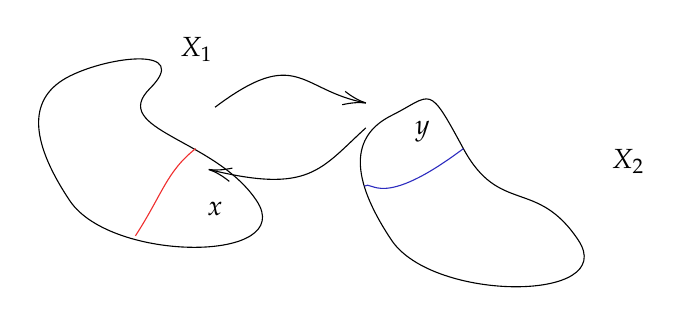
\begin{tikzpicture}[x=0.75pt,y=0.75pt,yscale=-1,xscale=1]
%uncomment if require: \path (0,249.36666870117188); %set diagram left start at 0, and has height of 249.36666870117188

\draw   (308,81) .. controls (328,71) and (325.3,64.9) .. (342.65,96.95) .. controls (360,129) and (378,111) .. (398,141) .. controls (418,171) and (328,171) .. (308,141) .. controls (288,111) and (288,91) .. (308,81) ;
\draw   (153,62) .. controls (173,52) and (211.65,47.95) .. (191.65,67.95) .. controls (171.65,87.95) and (223,92) .. (243,122) .. controls (263,152) and (173,152) .. (153,122) .. controls (133,92) and (133,72) .. (153,62) ;
\draw [color={rgb, 255:red, 239; green, 46; blue, 46 }  ,draw opacity=1 ]   (213.65,96.95) .. controls (199.65,107.95) and (197.65,118.95) .. (184.65,138.95) ;


\draw [color={rgb, 255:red, 45; green, 44; blue, 191 }  ,draw opacity=1 ]   (295,115) .. controls (298.65,111.95) and (302.65,126.95) .. (342.65,96.95) ;


\draw    (223,77) .. controls (263,47) and (263.65,68.95) .. (295.65,74.95) ;
\draw [shift={(295.65,74.95)}, rotate = 192.47] [color={rgb, 255:red, 0; green, 0; blue, 0 }  ]   (0,0) .. controls (3.31,-0.3) and (6.95,-1.4) .. (10.93,-3.29)(0,0) .. controls (3.31,0.3) and (6.95,1.4) .. (10.93,3.29)   ;

\draw    (295.65,86.95) .. controls (273.65,106.95) and (268.65,118.95) .. (220,107) ;
\draw [shift={(220,107)}, rotate = 373.35] [color={rgb, 255:red, 0; green, 0; blue, 0 }  ]   (0,0) .. controls (3.31,-0.3) and (6.95,-1.4) .. (10.93,-3.29)(0,0) .. controls (3.31,0.3) and (6.95,1.4) .. (10.93,3.29)   ;


\draw (214,49) node   {$X_{1}$};
\draw (223,126) node   {$x$};
\draw (422,103) node   {$X_{2}$};
\draw (323,89) node   {$y$};


\end{tikzpicture}

Glueing constructs $``X_1\cup X_2$ where each point $x$ is ``identified'' with the corresponding point $y$ in $X_2$.
\begin{figure*}[h]
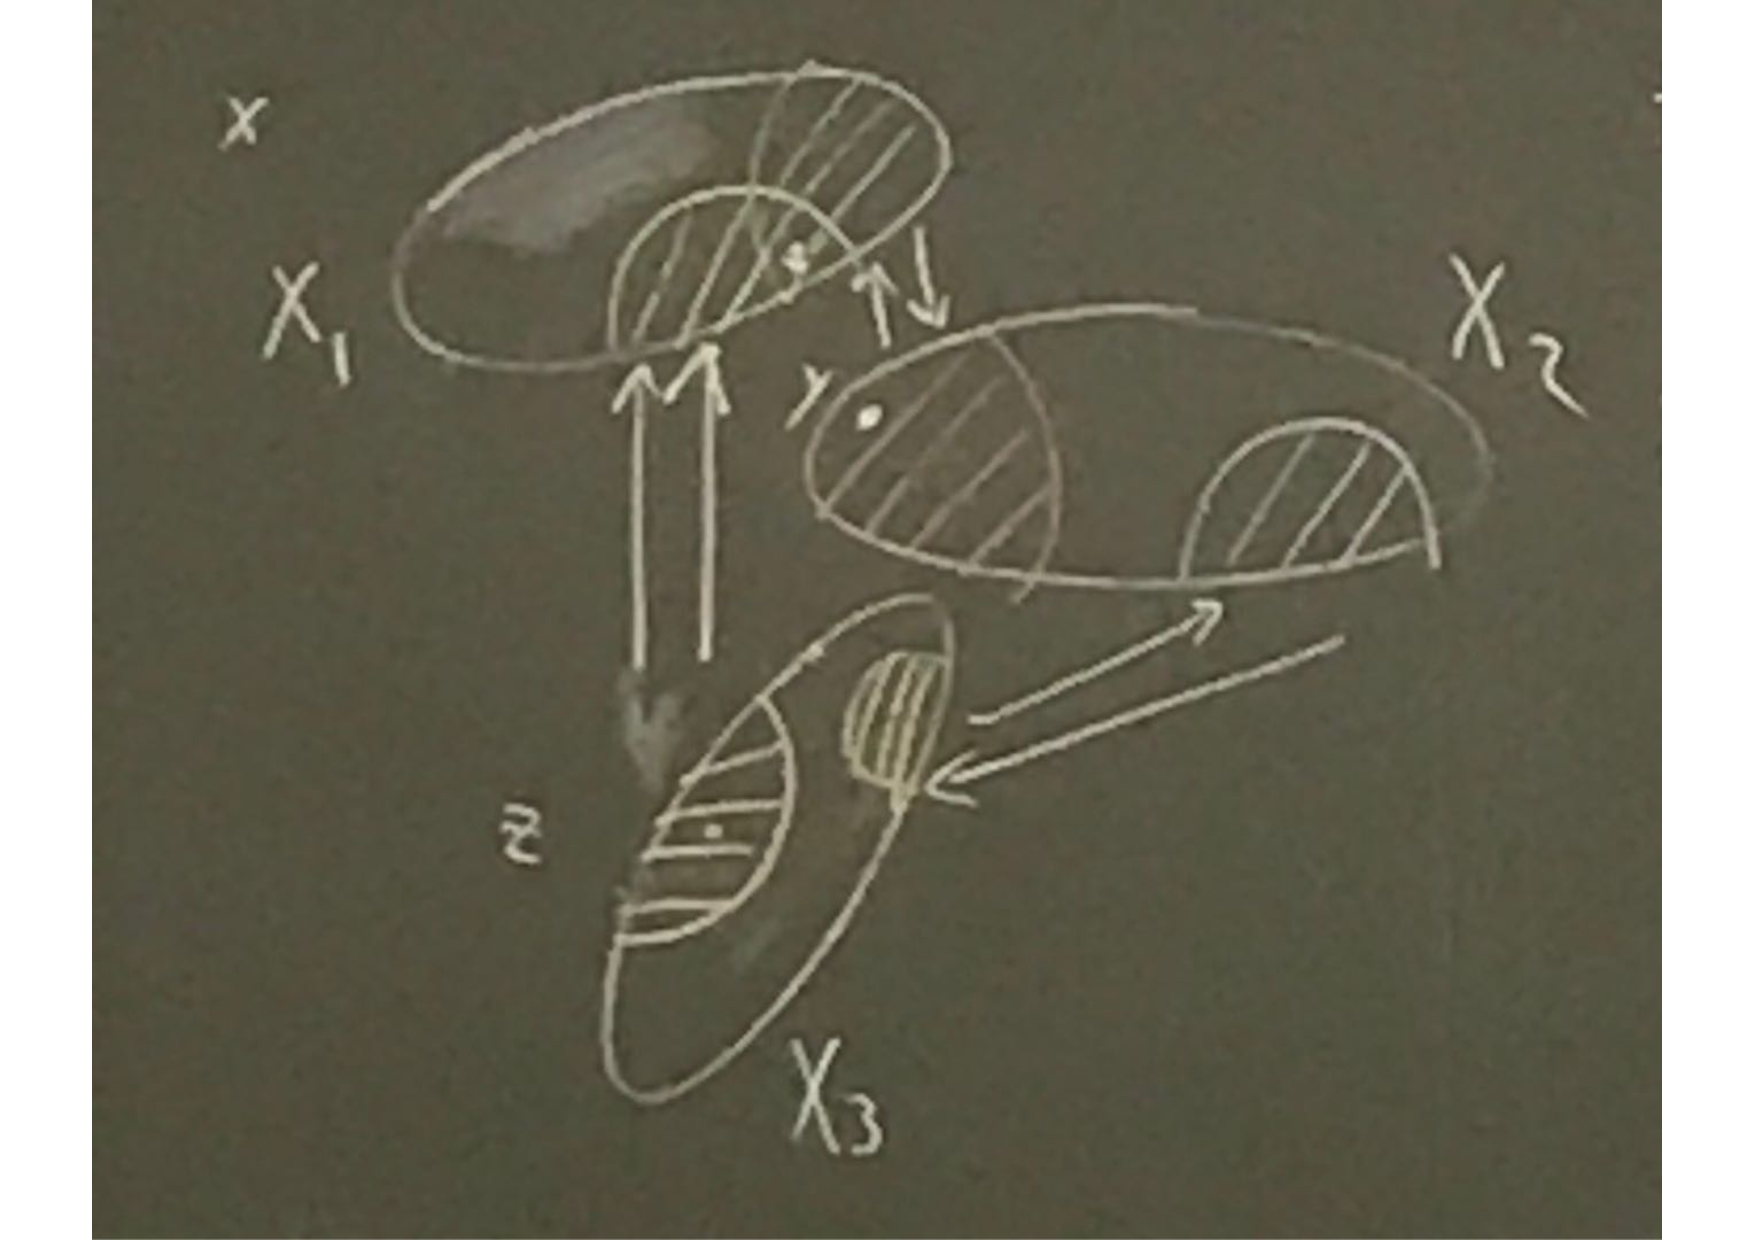
\includegraphics[width=0.2\textwidth]{cocycles.pdf}
\end{figure*}
More generally: we need to take care of intersections
>>>>>>>>>>1
\end{enumerate}
\begin{prop}
Given the glueing datum on $(X_i)_{i\in I}$, there is a scheme $X$ obtained by ``glueing the $X_i$'s along the $U_{ij}$ using $\varphi_{ij}$'s '' given by 
$$
X=\left(\sqcup_{i\in I}X_i\right)/\sim,
$$
where the equivalence relation is each $x\in X_i$ is identified with $\varphi_{ij}(x)\in X_{j}$ for $j\neq i$ if $x\in U_{ij}$, with the quotient topology. The quotient map $\sqcup X_i\overset{f}{\lrta} X$ is open, in particular $f(X_i)\subset X$ is open).

Note: $\sim$ is an equivalence relation because of the cocycle relation: if $y=\varphi_{ij}(x)$, then $x=\varphi_{ij}^{-1}(y)=\varphi_{ji}(y)$. If $y=\varphi_{ij}(x),x\in U_{ij},z=\varphi_{jk}(y), y\in U_{jk}$ and $x\in U_{ik}$, then $\varphi_{ik}(x)=\varphi_{jk}\circ \varphi_{ij}(y)=z$ so $x\sim y\sim z\Lrta x\sim z$ and with structure sheaf
$$
\calo_X(U)=\{(s_i)_{i\in I}|s_i\in \calo_{X_i}(U\cap X_i) \text{ s.t. } \varphi_{ij}^{\#}(s_{j}|U\cap U_{ji})=s_i|U\cap U_{ij}\},
$$
\begin{figure*}[h]
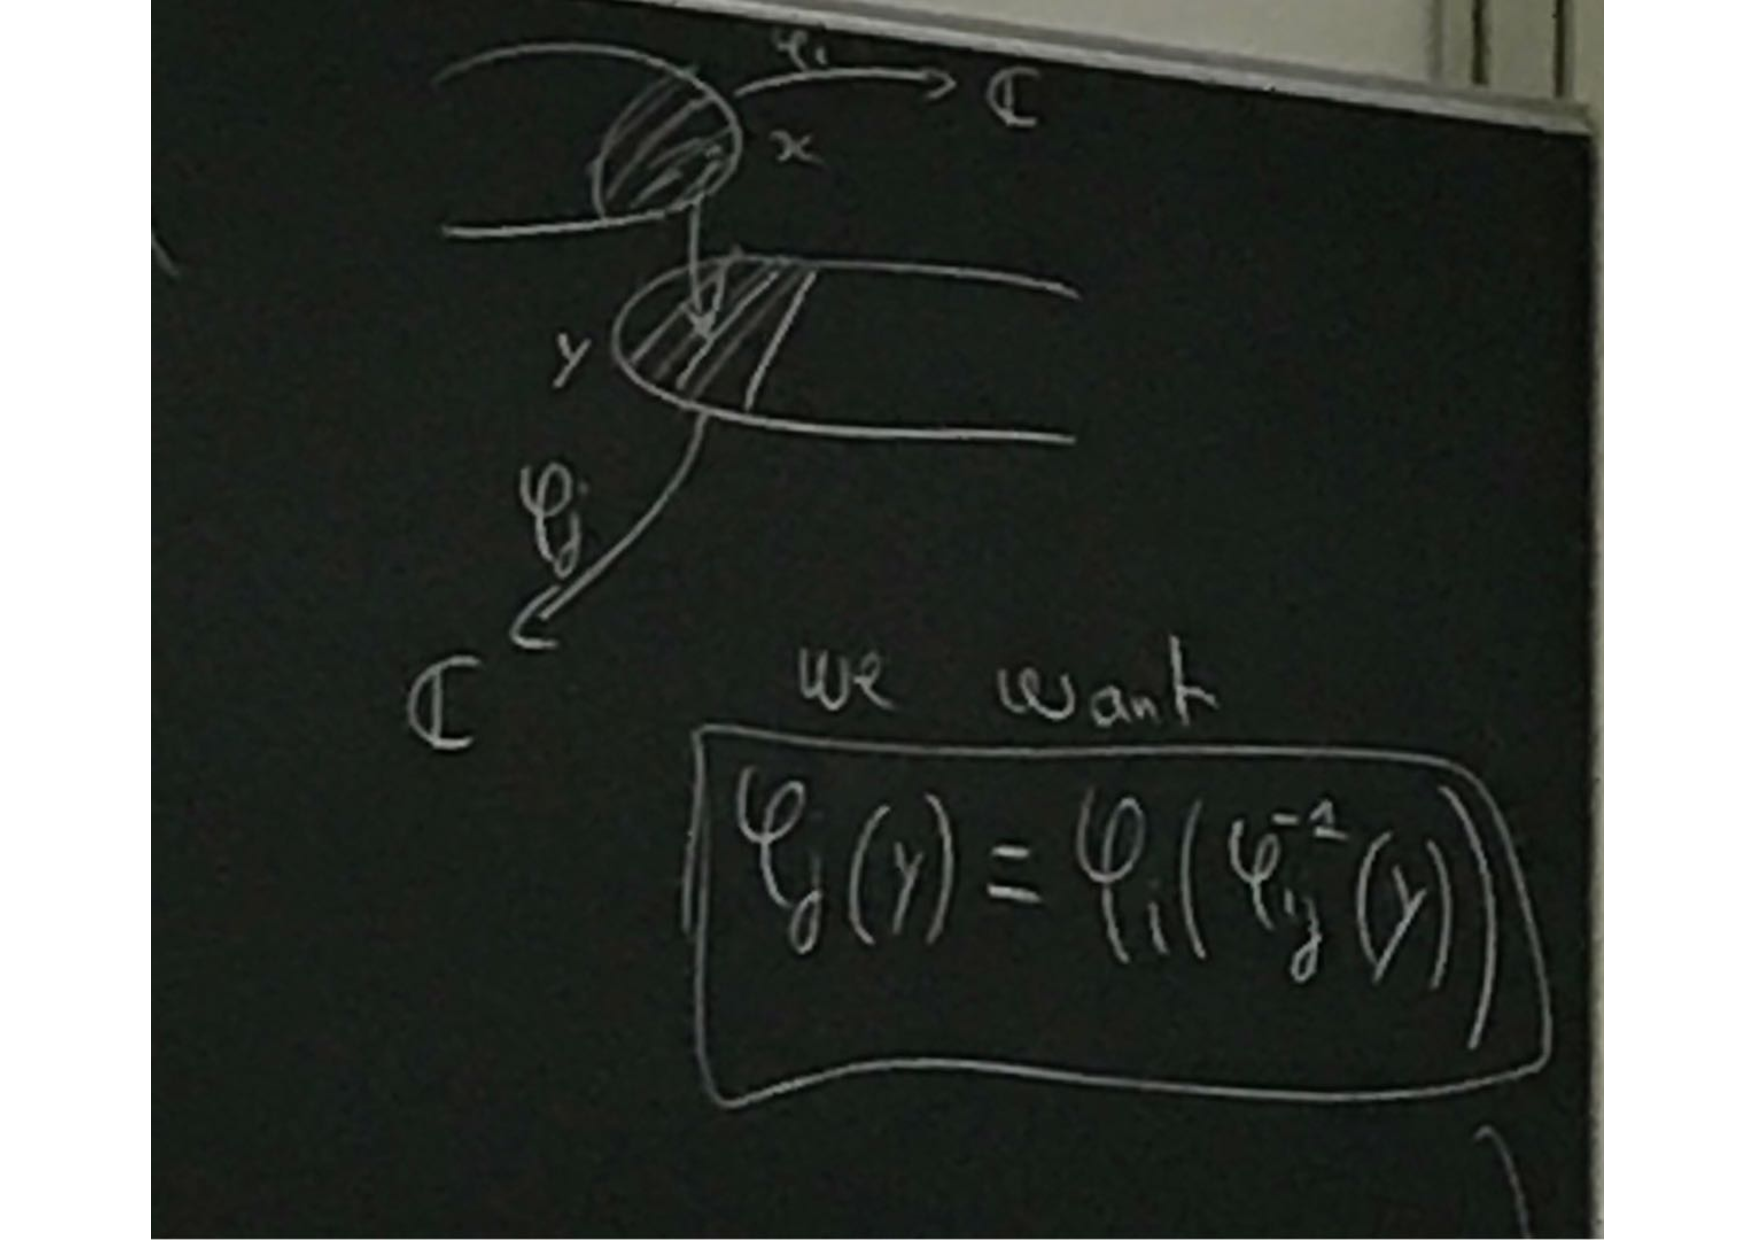
\includegraphics[width=0.3\textwidth]{pic2Aprl27.pdf}
\end{figure*}
we want
$s_j(y)=s_i(\varphi_{ij}^{-1}(y))$
\end{prop}
Note that the projection 
$$
f:\sqcup X_i\lrta X
$$ induces a homomorphism
$X_i\overset{\sim}{\lrta} f(X_i)\subset X$ with open image [$f|X_i$ is injective.]

We identify $X_i$ with $f(X_i)\subset X$ to write $U\cap X_i$ for instance (really it is $f^{-1}(U)\cap X_i$). Then $(X,\calo_X)$ is a ringed space  and there is an isomorphism 
$X_i\lrta f(X_i)$ of ringed spaces, it follows that(since $f(X_i)$ is open) that $X$ is a scheme.

Here we fix $j$,
$$
\calo_{f(X_j)}\lrta f_*\calo_{X_j}
$$
is given by 
$$
(s_i)\mapsto \text{ the unique $s$ section of $\calo_{X_j}$ that coincides with $s_i$ on} X_i\cap X_j=U_{ij}\subset X_i
$$
\underline{Application to } $\proj^n_\intg$. Let $A=\intg[X_0,...,X_n, X_0^{-1},...,X_n^{-1}]$. In $A$, we have subrings $A_i=\intg[\frac{X_0}{X_i},...,\frac{X_n}{X_i}]$. Note $A_i\simeq \intg[Y_1,..,Y_n]$ by 
$$
\begin{aligned}
&\frac{X_0}{X_i}\mapsto Y_1\\
&\frac{X_{i-1}}{X_i}\mapsto Y_{i}\\
&\frac{X_{i+1}}{X_i}\mapsto Y_{i+1}\\
&\frac{X_n}{X_i}\mapsto Y_n
\end{aligned}
$$
Let $X_i=\spec(A_i)$ ($\simeq \affn^n_\intg$), ($0\leq i \leq n$). Let $U_{ij}\subset X_i$ be $\spec\left((A_i)_{\frac{X_j}{X_j}}\right)=\spec (\intg[\frac{X_0}{X_i},...,\frac{X_n}{X_i},\frac{X_i}{X_j}])$ is an open subset in $X_i$.

Note that $B_{ij}=B_{ji}$, the identity $B_{ij}\lrta B_{ji}$ corresponds to an isomorphism 
$$
\varphi_{ij}:U_{ij}\lrta U_{ji}.
$$
Since the ring part is identity, the cocycle condition holds.
\begin{dfn}
$\proj^n_\intg$ is the glued scheme in that case
i.e. covered by $n+1$ open subschemes $\simeq \affn^n_\intg$, it is of finite type, Noetherian, integral ...
\end{dfn}
\begin{dfn}
$S$ is a  scheme, A \textbf{projective $S-$scheme}
$$
X\overset{f}{\lrta} S
$$
is a morphism such that there is a factorization
$$
X\overset{\text{closed immersion}}\inj \proj^n_S\lrta S
$$
for some integer $n\geq 1$.
\end{dfn}

How to concretely construct projective scheme over $K$? Let $K$ be a field,. Let $f\in K[X_0,...,X_n]$ homogeneous. \underline{Goal}: Define the zero set $Y$ of $f$ as a  closed subscheme of $\proj^n_K$. We are going to do it by glueing up the corresponding intersection
$$
Y\cap U_i
$$
We define the dehomogeneousation 
$$
f_i:=f\left(\frac{X_0}{X_i},..,1,..,\frac{X_n}{X_i}\right)\in K[\frac{X_0}{X_i},...,\frac{X_n}{X_i}]=A_i
$$
for $0\leq i\leq n$.
So we get \underline{closed immersions}
$$
Y_i=\spec(A_i/f_i A_i)\inj U_i
$$
Idea: $Y$ is obtained by glueing the $Y_i$ by identify $Y_i\cap U_{ji}$ with $Y_j\cap U_{ji}$ along $\varphi_{ij}$.

Precisely: Let $B_{ij}=K[\frac{X_0}{X_i},...,\frac{X_n}{X_i},\frac{X_i}{X_j}]$,
$$
Y_i\cap U_{ij}=\spec(B_{ij}/f_i B_{ij})
$$
and
$$
Y_i\cap U_{ij}=\spec(B_{ji}/f_j B_{ji})
$$
$$
\begin{tikzcd}
B_{ij} \arrow[r] \arrow[d, equal] & B_{ij}/f_iB_{ij} \arrow[d, "\sim"] \\
B_{ji} \arrow[r] & B_{ji}/f_jB_{ji}
\end{tikzcd}
$$
commutative because $f_i$ and $f_j$ generate the same ideal ub $B_{ij}=B_{ji}$, since
$$
\begin{aligned}
f_j &=\sum_J \alpha_J \left(\frac{X_0}{X_j}\right)^{d_0}\cdots\left(\frac{X_i}{X_j}\right)^{d_i}\cdots \left(\frac{X_n}{X_j}\right)^{d_n}\\
&=\sum_J \alpha_J \left(\frac{X_0}{X_i}\right)^{d_0}\cdots\left(\frac{X_i}{X_i}\right)^{d_i}\cdots \left(\frac{X_n}{X_i}\right)^{d_n}\cdot \left(\frac{X_j}{X_i}\right)^{d_0+\cdots d_n}\\
&= f_i \cdot \left(\frac{X_j}{X_i}\right)^{d_0+\cdots d_n}
\end{aligned}
$$



\subsection{May 4th-A: Projective schemes continued}
Recall: $\proj^n_\intg=$``glueing'' $U_i:=\spec(\intg[
X_0/X_i,..., X_n/X_i])$ along open subsets $U_{ij}=\spec(\intg[...]_{X_j/X_i})$

$f\in K[X_0,...,X_n]$ is non-constant homogeneous polynomial, $\leadsto$``vanishing scheme $Z_f$'' by  glueing the closed subschemes of $U_{i,K}=U_i\times_{\spec(\intg)}\spec (K)$ defined by $f_i=f(X_0/X_i,....,X_n/X_i)$. WE can do this with $f^{(1)},f^{(2)},....,f^{(m)}$ homogeneous of some degrees $\leadsto $ vanishing sets of finitely many homogeneous polynomials.

\underline{Fact}: These ``vanishing sets '' are closed subscheme of $\proj^n_K$ all closed subscheme of $\proj^n_K$ arise in this way.

\underline{Reason}: let $Y$ be this vanishing scheme; it is defined by glueing closed subschemes.
$$
Y_i\overset{\varphi_i}{\inj} U_{i,K}=\affn^n_K
$$
where 
$$
Y_i=\spec(K[X_0/X_i,...,X_n/X_i])/(f_i^{(1)},...,f_i^{(m)}).  
$$
One checks that there is a unique morphism
$$
\varphi:Y\lrta \proj^n_K
$$
such that  $\varphi|Y_i=\varphi_i$. and that $\varphi$ is a closed immersion. (Because every point has one $Y_i$ as an open neighbourhood
and $\varphi_i$ is a closed immersion.)

\begin{ex}
In $\proj^2_\intg$, we have a closed subscheme defined by 
$$
Y^2Z-X^3-XZ^2
$$
and on $U_2=\spec(\intg[X/Z,Y/Z,1])$ it is isomorphic to a closed subscheme of $\affn^2_n=\spec(\intg[U,V])$
$$
\left(\frac{Y}{Z}\right)^2-\left(\frac{X}{Z}\right)^3-\left(\frac{X}{Z}\right)=V^2-U^3-U.
$$
\end{ex}


\section{Divisors}
\subsection{May 4th-B: Weil divisors}
Divisors are the first non-trivial geometric invariants of the schemes and have many applications and forms.
\begin{itemize}
	\item classification of ``hypersurfaces'' in a scheme $X$. (Weil divisors.)
	\item certain sheaves (invertible sheaves of $\calo_X$-modules)
	\item Picard groups $\leadsto$ morphisms of projective spaces.
\end{itemize}

In order to define Weil divisors, the scheme is required to be Noetherian and integral. We usually look at those schemes with nice enough properties so that we don't have to worry about Cartier divisors
\begin{dfn}
Let $X$ be scheme. $X$ is \textbf{regular in codimension one} if for any $x\in X$ where $\dim(\calo_{X,x})=1$, the local ring $\calo_{X,x}$ is regular ($\dim \scm/\scm^2=1$). i.e. each local ring $\calo_{X,x}$ of dimension one is regular. (It's point of codimension at most one is regular, where the codimension of a point is defined to be the codimension of its closure.)
\end{dfn}

In this section, we require the scheme to be Noetherian integral, separated scheme which is regular in codimension one.
(In general a Noetherian local ring $(A,\scm)$, with $k=A/\scm$ is called regular if the dimension of $A$ is equal to the $\dim_k \scm/\scm^2$  this means $X$ has some minimal ``smoothness'')
\begin{ex}
\ \begin{enumerate}[label=(\arabic*)]
\item Assume, a scheme $X$ is of finite type over a filed $K$, then $X$ is regular in codimension one  if $X$ is ``non-singular'' in the sense analogue of definition of non-singular varieties.
\item $X=\affn_K^n=\spec(K[X_1,..,X_n])$. To say that $\scp\in X$ has dimension one means $\dim \calo_{X,\scp}=1\Llrta $ height of $\scp$ is equal to $1$. Because
$$
\calo_{X,\scp}=K[X_1,...,X_m]_{\scp} 
$$
in which prime ideals are exactly in bijection with prime ideals $\scq\subset \scp$. In $K[X_1,..,X_n]$ a prime ideal of height $1$ is principal ideal generated by $f$ irreducible. We also know that in that case $K[X_1,..,X_n]_{(f)}$ is regular.
\item $\proj^n_K$ is also regular in codimension $1$, because it is a local condition, and we apply $(2)$.
\item Any smooth curve over a field (points of dimension $1$ are closed points.)
\item If $X$ is a singular curve, it is not regular in codimension $1$.
\item $\spec(\intg)$ is also regular in codimension $1$. (the points of dimension $1$ are $p\intg$ and local ring  at $p\intg$ is 
$$
\calo_{\intg,p}=\left\{\frac{a}{b}\in \ratl| a,b \text{ coprime } and p\nmid b\right\}
$$
which is a regular local ring.
\end{enumerate}
\end{ex}
\underline{Convention:} Below in this section, $X$ is Noetherian, integral, regular in codimension $1$. (quasiprojective over affine base)
$$
X\underset{\inj}{\text{\tiny open}} Y\underset{\inj}{\text{\tiny closed }} \proj^n_S\lrta S
$$
In particular, $X$ is of finite type over $S$.

We look at closed subschemes of codimension $1$ in $X$.
\tikzset{every picture/.style={line width=0.75pt}} %set default line width to 0.75pt        

\begin{center}




\tikzset{every picture/.style={line width=0.75pt}} %set default line width to 0.75pt        

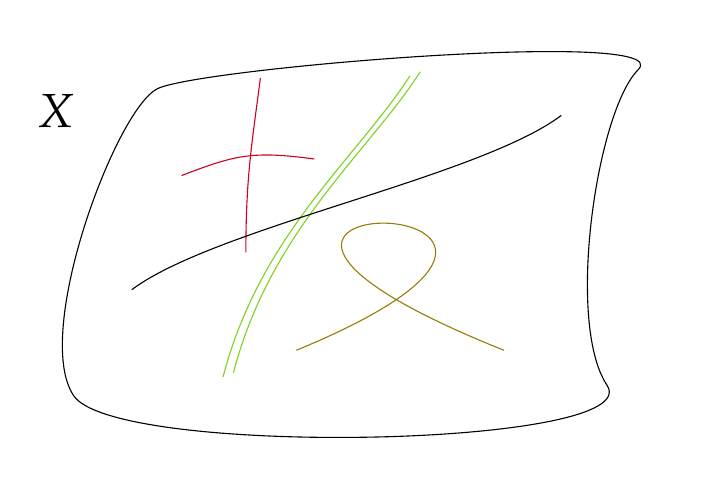
\begin{tikzpicture}[x=0.75pt,y=0.75pt,yscale=-1,xscale=1]
%uncomment if require: \path (0,300); %set diagram left start at 0, and has height of 300

\draw   (140,48) .. controls (160,38) and (391.65,18.85) .. (371.65,38.85) .. controls (351.65,58.85) and (336.65,160.85) .. (356.65,190.85) .. controls (376.65,220.85) and (119.65,225.85) .. (99.65,195.85) .. controls (79.65,165.85) and (120,58) .. (140,48) ;
\draw [color={rgb, 255:red, 149; green, 125; blue, 8 }  ,draw opacity=1 ]   (207,174) .. controls (398.65,94.85) and (96.65,89.85) .. (307,174) ;


\draw [color={rgb, 255:red, 126; green, 211; blue, 33 }  ,draw opacity=1 ]   (261.65,41.85) .. controls (236.65,80.85) and (189.65,117.85) .. (171.65,186.85) ;


\draw [color={rgb, 255:red, 208; green, 2; blue, 27 }  ,draw opacity=1 ]   (151.65,89.85) .. controls (177.65,79.85) and (185.65,77.85) .. (215.65,81.85) ;


\draw [color={rgb, 255:red, 208; green, 2; blue, 27 }  ,draw opacity=1 ]   (189.65,42.85) .. controls (185.65,73.85) and (182.65,89.85) .. (182.65,126.85) ;


\draw [color={rgb, 255:red, 126; green, 211; blue, 33 }  ,draw opacity=1 ]   (266.65,39.85) .. controls (241.65,78.85) and (194.65,115.85) .. (176.65,184.85) ;


\draw    (127.65,144.85) .. controls (167.65,114.85) and (294.65,90.85) .. (334.65,60.85) ;



\draw (91,59) node  [align=left] {{\LARGE $X$}};


\end{tikzpicture}

\end{center}

Regular codimension $1$ $\Lrta$ any such subscheme is a union of irreducible pieces, each of which is of the form $f^n=0$, $(n\geq 1)$ with $\{f=0\}$ being integral.

\begin{dfn}
\ \begin{enumerate}[label=(\arabic*)]
\item  A \textbf{prime (Weil) divisor} $D$ in $X$ is an integral closed subscheme of codimension $1$. (there is no intermediate closed subscheme between $D$ and $X$)~\footnote{In some reference, it is also defined to be irreducible closed subscheme of codimension $1$ only, but recall that there is always a reduced subscheme structure on closed subset}
\item The \textbf{group of Weil divisors} on $X$ is the free abelian group generated by  prime divisors.
$$
\sum_{i\in I, finite} n_i D_i
, n_i\in \intg\text{ and } D_i \text{ prime divisors }
$$
It is denoted $\text{Div}(X)$. A divisor $D=\sum_i n_i D_i$ is effective if all $n_i\geq 0$. Intuitively, effective divisor $\sum_i n_i D_i$ corresponds to the closed subscheme union of the $D_i$'s with multiplicity $n_i$.
\end{enumerate}
\end{dfn}
\begin{dfn}
The \textbf{function field} of an integral scheme $X$ is the residue field/local ring at the generic point $\eta$ of $X$. An element $f$ of $K(X)$ is therefore the equivalence class of $(U,s)$ where $U$ is 
an open set $\emptyset \neq U\subset X$ and $s\in \Gamma(U,\calo_X)$, $(U,s)\sim (V,t)$ iff $s|_{U\cap V}=t|_{U\cap V}$.
\end{dfn}
\begin{ex}
$K(\affn^n_K)=K(X_1,...,X_n)=K(\proj^n_K)$
\end{ex}
\begin{lemma}
Let $D$ be a prime divisor, and $\eta_D$ its generic point. Let $\tilde{\eta}_D$ be the image of $\eta_D$ in $X$. The ring 
$\calo_{X,\tilde{\eta}_D}$ is a DVR with fraction field $K(X)$
\end{lemma}
\begin{proof}
\underline{Affine Case}: $D=\spec(A/\scp)$ with $\scp$ prime ideal so that $A/\scp$ is integral. $\eta_D=\{0\}\subset A/\scp$ and $\tilde{\eta}_D=\scp\in \spec(A)$.

$D$ has codimension $1$, $\Llrta$ $\text{ht}(\scp)=1\Llrta \dim \calo_{X,\tilde{\eta}_D}=\dim A_\scp=1$. So, by regularity in codimension $1$, $A_\scp$ is a regular local ring of dimension $1$, Noetherian, i.e. it is a DVR $\Llrta $ [maximal ideal is principal. ] Then $K(X)=Frac(A)=Frac(A_\scp)$. 

In general, we don't need to reduce other case to the affine case to argue it is a DVR. Because $D$ is irreducible and of codimension $1$, and $X$ is Noetherian integral scheme which is regular in codimension $1$. We know $\calo_{X,\tilde{\eta}_D}$ is regular local $1$-dimensional Noetherian domain. A theorem of commutative algebra says it is a DVR.

This point $\tilde{\eta}_D$ is contained in some affine open $\spec A$, where $A$ is an integral domain, and we recall that any $Frac(A_\scp)=Frac(A)$ for every prime $\scp \subset A$. On the other hand $\spec A$ is dense in $X$, we have $Frac(A)=K(X)$. This works for any  integral scheme. (The residue field of each point in an integral scheme is the function field.)
\end{proof}

Now given $D$ a prime divisor, $f\in K(X)^{\times}$, we denote by $\nu_D(f)$ the valuation at $D$ of $f$, $f\in Frac(\calo_X,\tilde{\eta}_D)$. $(\scm_{X,\tilde{\eta}_D} =(\varpi))$ then $f\in Frac(\calo_{X,\tilde{\eta}_D})$ is of the form $\frac{a}{b}$, $a, b$ in $\calo_{X,\tilde{\eta}_D}$, 
$a=\varpi^n u, n\geq 0, u\in\calo_{X,\tilde{\eta}_D}^\times$ and $b=\varpi^m v, m \geq 0, v\in\calo_{X,\tilde{\eta}_D}^\times$ and $\nu_D(f)=n-m$.

\underline{Intuitively:}
$d=\nu_D(f)\geq 1$ means $f$ has a zero of order $d$ along $D$ ( has degree of vanishing $d$ along $D$). $d\geq -1$ means a pole of order $-d$ (a zero of order $d$ of $1/f$)



\begin{lemma}[Hartshorne II 6.1]\label{lem:Hartshorne II.6.1} If $f\in K(X)^\times$ then $\nu_D(f)=0$ for all but at most finitely many prime divisors $D$.
\end{lemma}
\begin{proof}[Proof of Lemma~\ref{lem:Hartshorne II.6.1}]
Let $f\in K(X)^\times$, view it as $f\in \Gamma(U,\calo_X),$ where $\emptyset \neq U=\spec(A)$ is affine. Let $Z=X-U$, closed in $X$, with reduced subscheme structure.

$\{D\text{ prime }\mid D\subset Z \}$ is finite because $X$ (hence $Z$) is  Noetherian.

Example. $f=X^2+3X^2Y+Y^3/(XY)$, $Z=$ union of coordinate axes, each is prime. If $D$ is not in $Z$ then $U\cap D=D_U$ is non-empty, and hence dense in $D$.

 \underline{Claim}: $U\cap D$ is a prime divisor in $U$.

  Then $\nu_{D\cap U}(f)[=\nu_D(f)]\geq 0$ since $f\in \Gamma(U,\calo_X)=A$ and to say that $\nu_{D\cap U}(f)\geq 1$ means $D\cap U\subset V(fA)$ proper closed in $U$. So again this happens for finitely many $D$.

Why is $U\cap D$ a prime divisors in $U$?
\begin{center}


\tikzset{every picture/.style={line width=0.75pt}} %set default line width to 0.75pt        

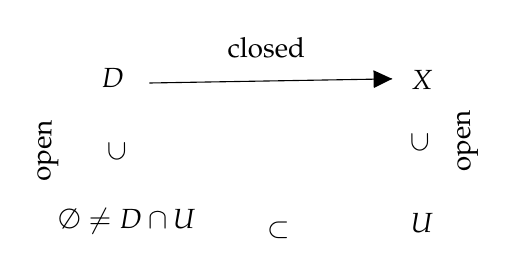
\begin{tikzpicture}[x=0.75pt,y=0.75pt,yscale=-1,xscale=1]
%uncomment if require: \path (0,300); %set diagram left start at 0, and has height of 300

\draw    (196.65,66.25) -- (313.65,64.25) ;
\draw [shift={(313.65,64.25)}, rotate = 539.02] [fill={rgb, 255:red, 0; green, 0; blue, 0 }  ] [draw opacity=0] (8.93,-4.29) -- (0,0) -- (8.93,4.29) -- (8.93,-4.29)    ;


\draw (179,64) node   {$D$};
\draw (186,133) node   {$\emptyset \neq D\cap U$};
\draw (328,65) node   {$X$};
\draw (328,134) node   {$U$};
\draw (181,99) node [rotate=-269.62]  {$\subset $};
\draw (327,95) node [rotate=-269.62]  {$\subset $};
\draw (259,137) node   {$\subset $};
\draw (148,99) node [rotate=-271.46] [align=left] {open};
\draw (350,94) node [rotate=-269.51] [align=left] {open};
\draw (253,49) node  [align=left] {closed};


\end{tikzpicture}

\end{center}
$D\cap U$ is an open subscheme of $D$ then check that $D\cap U\simeq D\times_X U$, so $D\cap U\inj U$ is a closed immersion. Moreover $D\cap U$ is integral because $D$ is integral. One checks that $D\cap U$ is also of codimension $1$
$$
K(U)=K(X)
$$
$$
\Lrta \nu_{D\cap U}(f)=\nu_D(f).
$$
\end{proof}
\begin{dfn}
For 
$f\in K(X)^\times$,
$$
\div(f)=\sum_{D\text{ prime}} \nu_D(f) D \in \text{Div}(X)
$$
$$
div:K(X)^\times\lrta \text{Div}(X)\text{ group morphism }
$$
The group of all $\div(f) $ is called the group of \textbf{principal divisors}. The quotient
$$
\text{Div}(X)/Im(div)=\text{Cl}(X)
$$
is the \textbf{divisor class group } of $X$.
\end{dfn}


\subsection{May 8th-A: Divisors class group}

Reminder:
 Let $X$ be a scheme, which is integral regular in codimension one, Noetherian, quasi-projective.

 We defined $\Div(X):=$ free Abelian group with basis of the integral codimension 1 subschemes.

 $f\in K(X)^\times$

 $\Lrta \div(f)=\sum_D \nu_D(f)D$
 
 $div$ gives a group morphism $K(X)^\times\lrta \Div(X)$

\begin{dfn}
$Cl(X)=\Div(X)/Im(div)$ is called the \textbf{divisor class group}.
\end{dfn}
\begin{ex}\ 
\begin{enumerate}[label=(\arabic*)]
\item
Let $X$ be  a smooth curve over a field $K$
$\Lrta$ prime divisors are closed points of $X$, an $f\in K(X)^\times$ can be seen as a non-constant morphism 
$$
f:X\lrta \proj^1_K
$$
and $\div(f)=$zero of $f$ with multiplicities or poles of $f$ with multiplicities.

$Cl(X)\llrta$ ``given points $x_1,...,x_m$ and$y_1,...,y_n$  with specified integers of $\nu_1,..,\nu_m\geq 1$ and $\mu_1,...,\mu_n\geq 1$''. Is there an 
$$
f: X\lrta \proj^1_K
$$
s.t. $f$ has zeros at $x_i$ with multiplicities $\nu_i$ and poles at $y_j$ with multiplicities $\mu_j$

$\leadsto$ \textbf{Riemann-Roch Theorem}
\item $X=\affn^1_K=\spec(K[T])$. Prime divisors is in one to one correspondence with irreducible monic polynomials in $K[T]$ and divisor can be identifies to $f_1/f_2$, where $f_1,f_2$ are coprime monic polynomials. By $\sum n_i D_i\mapsto \prod_i f_i^{n_i}$ 
(This is historically one of the motivating cases)
\item $X=\affn^n_K$ (or $\affn^n_\intg$)
\underline{Claim}: $Cl(X)=0$.
(In fact: prop II 6.2 in Hartshorne If $A$ is, integral domain and integrally closed , then $A$ is $UFD$ $\Llrta Cl(\spec(A))=0$)

Any prime divisor $D$ in $\affn^n_K$ is of the form $V((f))$ for $f\in A$ irreducible, thus $D=\spec(A/(f))$.

 Let $D=\sum n_i D_i$ be a divisor with $n_\geq 1$, $D_i$ distinct. We can define $f_i$ so that
 $$
D_i=\spec(A/(f_i))
 $$
 and let $f=\prod f_i^{n_i}\in K(T_1,...,T_n)^\times=K(\affn^n_K)$.
 Then recall how to compute $\div(f)$: $D$ prime divisor, $D=\spec(A/(g))$
 $$
 \begin{aligned}
 \calo_{\affn^n_K,\tilde{\eta}_D}
 &=A_{(g)}\\
 &=\{f_1/f_2\in K(T_1,..,T_n)^\times: g\nmid f_2\}
 \end{aligned}
 $$
 is indeed a DVR with maximal ideal generated by $g$, and $\nu_D(f_1/f_2)=$ the exponent of $g$ $=k$ s.t. 
 $f_1/f_2=g^k u$, with $u\in A_{(g)}^\times$. So $\div(f)=\sum n_i D_i=D$ so any $D$ is principal, therefore $Cl(\affn^n_K)=0$

\item $Cl(\spec K)=\{0\}$ has no prime divisors. Consider $L/\ratl$ finite extension. Let $A\subset L$ be the integral closure of $\intg$. Then $\spec(A)$ is regular of codimension one, so 
$
Cl(\spec A)
$
is defined.
This is isomorphic to the ``ideal class group'' $H(L)$ of $L$.

We sketch the reason here.
$$
H(L)=\{\text{fractional ideals}\}/\{\text{ principal ideals}\}
$$
where $\{\text{fractional ideals}\}\simeq\text{free Abelian group generated by prime ideals}$ and  a fractional ideal is principal iff it is associated to a principal ideal.

There are still many open questions: are there infinitely many $L/\ratl$ with $Cl(\spec A)=0$? (i.e. $A$ UFD)

How are $Cl(\spec A)$ distributed when $L/\ratl$ varies? (Cohen-Lenstra Heuristics)

\item $X=\proj^n_K$ with $K$ is a field.

\underline{Fact}: the prime divisors are the closed subschemes associated to a single homogeneous irreducible polynomials $f\in  K[X_0,..,X_n]$.
\begin{thm}
(II 6.4) Define a group morphism from the $\underline{deg}: \Div(X)\lrta \intg$
$$
D\longmapsto deg(f)
$$ 
where $D$ is the subscheme associated to homogeneous polynomial $f$.
\begin{enumerate}[label=(\alph*)]
\item For all principal divisors $\div(f), f\in K(X)$, we have $\underline{deg}(\div f)=0$.
\item The induced morphism from class groups to $\intg$ 
$$
Cl(X)\overset{\underline{deg}}{\lrta }\intg
$$
is  an isomorphism.
\item $Cl(X)$ is isomorphic to $\intg$ with generator any 
$$
H_i=\proj^n_K-U_i
$$
where $U_i$ is  the canonical affine chart of $\proj^n_K$ corresponding to $X_i$
\end{enumerate}
\end{thm}
\begin{proof}
\begin{enumerate}[label=(\alph*)]
\item (A function on $\proj^n_K$ has the same number of zeros and poles with multiplicities) We know
$$
K(X)^\times=K(U_0)^\times
$$
where $U_0=\spec(K[X_0/X_0,X_1/X_0,..,X_n/X_0])$. So $K(X)=K(X_0/X_0,...,X_n/X_0)$
So $f\in K(X)^\times$ is of the form $f=f_1/f_2$ where $f_i \in K[X_0/X_0,..,X_n/X_0]$. 

\underline{Key fact}: 
We can also express $f=g_1/g_2$ where $g_i$ is homogeneous of degree $deg g_1=deg g_2$ in $K[X_0,..,X_n]$. Then factor $g_1,g_2$ in irreducibles in $K[X_0,..X_n]$, there are homogeneous, say 
$$
f=\prod_i h_i^{n_i}\prod_j k_j^{-m_j}
$$
with $n_i\geq 1, m_j \geq 1$
Then 
$$
\div(f)=\sum n_i D_i-\sum m_j E_j
$$
and $D_i$ is the prime divisors of $h_i$, $E_j$ is the prime divisors of $k_j$. (Intuitively, it is clear, but we need a proof)

$\Lrta$
$$
\begin{aligned}
\underline{deg}(\div(f))&=\sum n_i \underline{deg}(D_i-\sum m_j \underline{deg}(E_j)\\ 
&(\underline{deg}(D_i)=deg(h_i),\underline{deg}(E_j)=deg(k_j))\\
&=deg(g_1)-deg(g_2)=0.
\end{aligned}
$$
Then we come back to prove the \underline{Key fact}:
$$
f_1=\sum_{\underline{d}}\alpha_{\underline{d}} \left(\frac{X_0}{X_0}\right)^{d_0}\cdots \left(\frac{X_n}{X_0}\right)^{d_n}
$$
e.g.
$$
\begin{aligned}
&\left(\frac{X_1}{X_0}\right)^{2}+37 \left(\frac{X_1}{X_0}\right)^{3}\left(\frac{X_2}{X_0}\right)\\
&=\frac{X_0^2X_1^2+37X_1^3X_2}{X_0^4}\\
&=\frac{1}{X_0^{deg f_1}}\sum_{\underline{d}}\alpha_{\underline{d}} X_0^{deg f_1-\sum_{i=1}^n d_i} X_1^{}d_1\cdots X_n^{d_n}\\
&=\frac{\text{homogeneous degree $deg f_1$}}{X_0^{deg f_1}}\\
\end{aligned}
$$
$$
\Lrta f_2=\frac{\text{homogeneous degree $deg f_2$}}{X_0^{deg f_2}}\\
$$
$$
\Lrta \frac{f_1}{f_2}=\frac{X_0^{ deg f_1}(deg f_1)}{(deg f_2) X_0^{deg f_1}}
$$

\item $\underline{deg}: Cl(X)\lrta \intg$ is surjective because $\underline{deg}(D_0)=1$, $D_0$ associated to $X_0$ and injective because if $deg(D)=0$ write $D=D_1-D_2$ with $D_1,D_2$ effective then $\underline{deg}(D_1)=\underline{deg}(D_2)$. Write 
$D_1=\sum n_i E_i$, where $E_i$ is prime divisors associated to $h_i$. 
$D_2=\sum m_j F_j$, where $F_j$ is prime divisors associated to $k_j$. 


Then let $f=\prod h_i ^{n_i}\prod k_j^{- m_j}\in K(X)^\times$, and as shown above $\div(f)=D_1-D_2=D$ so $D$ is  $0$ in $Cl(X)$.
\item follows from $(a)$ and $(b)$ and the fact that $\underline{deg}(H_i)=deg(x_i)=1$
\end{enumerate}
\end{proof}
\item Further examples: 
\begin{enumerate}[label=(\alph*)]
\item $X\subset \proj^4_K$ cubic, where $K$ is an algebraic closed field. $X$ is a  surface, smooth, then $\pic(X)\simeq \intg^7$
\item $Y\subset \proj^2_K$ curve of degree $d$. Let $U\subset \proj^3_K-Y$ be the complements, then 
$$
Cl(U)\simeq \intg/d\intg
$$
generated by $U\cap H_0$
\end{enumerate}
\end{enumerate}
\end{ex}

\section{Invertible sheaves and Picard group}
\subsection{May 8th-B: Picard group, definitions}
\begin{dfn}
Let $(X,\calo_X)$ be a ringed space. A \textbf{sheaf of $\calo_X$-modules} is a sheaf
$\calf$ on $X$ so that $\calf(U)$ is a $\calo_X(U)$-module for any open $U$ and for $V\subset U$
$$
\calf(U)\overset{\res}{\lrta}\calf(V)
$$
is linear i.e. given $f\in \calo_X(U), s\in \calf(U)$
$$
\res (f s)=\res(f)\res(s)
$$
\end{dfn}

One defines in an obvious way $\calo_X$-linear morphism of $\calo_X$-modules
[$\forall U, \calf_1(U)\lrta\calf_2(U)$ is $\calo_X(U)$-linear], so ther is a category of $\calo_X$-modules
\begin{ex}
$n\geq 1$, $\calo_X^n:U\lrta \calo_X(U)^n$ is an $\calo_X(U)$-module. 
\end{ex}
\begin{dfn}
An $\calo_X$-moduel $\calf$ is \textbf{locally free} of rank $n\geq 1$ is $\forall x\in X,\exists U $ open nbhd of $x $ s.t.
$$
\calf|_U\simeq \calo_U^u
$$
as sheaves of $\calo_U$-module.
\end{dfn}

If $\call$ is  locally free of rank $1$, it is called an invertible sheaf.
\begin{prop}
The set $\pic(X)$ of isomorphism class of invertible sheaves on $X$ form  an abelian group with operation induced by 
$$
(\call_1,\call_2)\longmapsto \call_1\otimes_{\calo_X}\call_2
$$
$$
\text{$1=$ class of $\calo_X$}
$$
$$
\text{inverse }
\call\longmapsto \hom_{\calo_X}(\call,\calo_X)
$$
N.B for $\calf_1,\calf_2$ $\calo_X$-modules, we define
$$
\calf_1\otimes_{\calo_X}\calf_2=\text{ sheaf associated to  the presheaf $U\mapsto \calf_1(U)\times_{\calo_X(U)}\calf_2(U)$}
$$
and
$$
\hom_{\calo_X}(\calf_1,\calf_2)=\text{ sheaf associated to $U\mapsto \hom_{\calo_X(U)}(\calf_1(U),\calf_2(U))$}
$$
\end{prop}


\subsection{May 11th: The twisting invertible sheaf $\calo(m)$ on $\proj^n$}

Recall:
$\calo_X$-modules, locally-free $\calo_X$-modules,

rank $1$ locally free $\Lrta$ invertible sheaves.

\begin{prop}
$\pic(X)=\{\text{iso. class of  invertible sheaves}\}$ is an abelian group with $\call_1\otimes \call_2$
and $1=\calo_{X}$, $\call^{-1}=\phom(\call,\calo_X)$.
\end{prop}
\begin{proof}
What needs to be done (given commutativity/ Associativity of $\otimes$) is
\begin{enumerate}[label=(\arabic*)]
\item if $\call_1,\call_2$ are invertible, so is $\call_1\otimes \call_2$
\item $\call\otimes \calo_X=\call$
\item $\call\otimes \call^{-1}\cong \calo_X$.
\end{enumerate}

$(1)$: If $\call_1|_U\simeq \calo_X|_U$ and $\call_2|_U\simeq \calo_X|_U$,  $(\call_1\otimes\call_2)|_U\simeq \calo_X|_U\otimes\calo_X|_U\simeq \calo_X|_U$, where the LHS is sheaf associated to presheaf, (given $V\subset U$) $V\longmapsto\call_1(V)\otimes\call_2(V)$ and the $\calo_X(V)\otimes \calo_X(V)\simeq \calo_X(V)$. So the LHS is the sheaf $V\longmapsto \calo_X(V)$ and $\call_1|_U\otimes \call_2|_U\simeq \calo|_U$ and therefore $\call_1\otimes \call_2$ is invertible.

\underline{Warning!} in general, $\call_1\otimes \call_2(U)\neq\call_1(U)\otimes\call_2(U)$.

$(2)$ For any $U\subset X$, 
$$
\call(U)\otimes\calo_X(U)\overset{\sim}{\lrta}\call(U)
$$
$$
(s,a)\longmapsto as
$$
$\Lrta $ a morphism of presheaves 
$$
[U\mapsto \call(U)\otimes\calo_X(U)]\longmapsto \call
$$
$\Lrta$  a canonical morphism
$$
\call\otimes\calo_X\longmapsto \call
$$
and this is  an isomorphism because on stalks it is 
$$
\call_x\otimes \calo_{X,x}\simeq \call_x
$$
$$
(s,a)\longmapsto as
$$
which is an isomorphism

$(3)$ For any $U\subset X$ we have an isomorphism of modules
$$
\call(u)\otimes\call^{-1}_{pre}(U)\overset{\sim}{\lrta}\calo_X(U)
$$
$$
LHS=\call(U)\otimes\hom_{\calo_X(U)}(\call(U),\calo_X(U))
$$
$$
(s,\lambda)\longmapsto \lambda(s).
$$
After sheafification, we get a morphism
$$
\call\otimes\call^{-1}\lrta \calo_X
$$
which at stalks is an isomorphism.
\end{proof}


\begin{ex}\ 
\begin{enumerate}[label=\boxed{\arabic*}]
\item \underline{Affine case}: $X=\spec A$. Theory of (quasi)-coherent sheaves establishes
 a connection between $A$-modules and $\calo_X$-modules.

Given an $A$-module $M$, we can construct a $\calo_X$-module  $\tilde{M}$ by 
$$
\tilde{M}(U)=\left\{s:U\lrta \sqcup_{x\in U}M_x\left|\begin{aligned}
&\forall x,s(x)\in M_x, \forall x\in U,\exists V\subset U
,\\
&\text{s.t. for } x\in V,\exists m\in M,\exists f\in A,\\ 
&\text{ s.t. } \forall y\in V f\notin y,\  s(y)=\frac{m}{f}\in M_y  
\end{aligned}
\right.\right\}
$$
subexample: $\tilde{A}=\calo_X$ and $\tilde{M}$ is an $\calo_X$-module:
$$
(a\cdot s)(x)=a(x)s(x)
$$
for all $a\in \calo_X(U), s\in \tilde{M}(U)$

\underline{Facts:}

\begin{enumerate}
\item $\Gamma(U_f,\tilde{M})\simeq M_f\lrta $``$f(x)\neq 0$''
\item stalk $\tilde{M}_x= M_x$ localization
\item $\widetilde{M_1\otimes M_2}=\tilde{M_1}\otimes\tilde{M_2}$
\item  [Serre-Swan] Locally-free $\calo_X$-modules is in bijection with vector bundle and  projective $A$-modules.

In practice, $\tilde{M}$ is an invertible sheaf iff $M$ is projective, locally of rank $1$ $M_\scp\cong A_\scp$ (when viewed as $A_\scp$-module)

\underline{Cor}: If $A$ is a UFD, then $Pic(\spec A)=\{0\}$
\end{enumerate}

\item If $X$ has the usual regularity properties, and $D$ is a prime divisor, there is a naturally associated invertible sheaf $\call(D):$ Let $U\subset X$ open small enough, so that $D\cap U$ is given by $f=0$ on $U$, then
$$
\call(D)(U)=\{s\in Frac(\calo_X(U))| s=f^{-1}t, t\in \Gamma(U, \calo_X)\}
$$
 One checks that this is well-defined (it is independent on the choice of $f$)

 Then $\call(D)$ is an invertible sheaf. This extends to a group morphism
 $$
  \Div(X)\lrta Pic(X).
 $$
 \item The twisting sheaf on projective space. Let $K$ be a field. We define an important non-trivial invertible sheaf on $\proj^n_K$, $n\geq 1$, denoted 
 $$
\calo(1)=\calo_{\proj^n_K}(1).
 $$

 From the $\Proj$ point of view, where $K[X_0,..,X_n]=:A$
 $$
\proj^n_K=\Proj(A)
 $$
$$
\begin{tikzcd}
M \arrow[d,rightsquigarrow] & \text{graded } A\text{-module} \\
\tilde{M} & \calo_{\Proj(A)}\text{-module}
\end{tikzcd}
$$
Take: 
$$
M=\bigoplus_{k\geq 1}A_k,
$$
where $A_k$ is the homogeneous part of degree $k$.
$\Lrta \tilde{M}=\calo(1)$.

Glueing: $n$,
$$
\proj^n_K=\cup_{i=0} U_i
$$
where $U_i=\spec(B_i)$, $B_i=K[X_0/X_i,...,X_n/X_i]\subset B=[X_0^{\pm },..,X_n^{\pm}]$
glued over $U_{ij}=\spec(B_{ij})$, with $B_{ij}=(B_i)_{X_j/X_i}$ using the isomorphism 
$$
B_{ij}=B_{ji}\subset B.
$$
To define a sheaf $\calf$ on $\proj^n_K$ it suffices to consider sheaves $\calf_i$ on $U_i$, isomorphisms $\varphi_{i,j}\calf_i|_{U_{ij}}\simeq \calf_{j}|_{U_{ij}}$ with the cocycle condition on $\varphi_{i,j}$. We define $\call_i$ on $U_i$ by 
$$
\call_i=\tilde{M}_i
$$
where $M_i=X_i B_i\subset B_i$ as $B_i$-module. We have 
$M_i\simeq B_i$ as $B_i$-module so $\tilde{M}_i\simeq \calo_{\proj^n}|_{U_i}$ we glue the $\call_i$
 over $U_{ij}$ using the isomorphisms 
 $$
B\supset M_{i,\left(\frac{X_j}{X_i}\right)}=M_{j,\left(\frac{X_i}{X_j}\right)}.
 $$
 These identity morphisms glue to an ivertible sheaf $\calo(1)$ on $\proj^n_K$. By \boxed{1}, we have 
 $$
 \Gamma(U_i,\calo(1))\cong \Gamma(U_i,\tilde{M}_i)=M_i=X_i B_i.
 $$
 \begin{prop}
 We have 
 $$
\dim_K \Gamma(\proj^n_{K},\calo(1))=n+1
 $$
 and $\dim_K\Gamma(\proj^n_K,\calo)=1$. (A basis of $\Gamma(\proj^n_K,\calo(1))$ is given by the ``homogeneous coordinates'')
 \end{prop}
 \begin{proof}
 Using the glueing perspective $s\in \Gamma(\proj^n_K,\calo(1))$ is equivalent to $(s_i), s_i\in \Gamma(U_i,\calo(1))$ with $s_i|_{U_{ij}}=s_j|_{U_{ji}}$ which means 
 $$
 s_i\in M_i=X_i B_i\subset B
 $$
 and $s_i=s_j$ in $B$.
 $\Lrta$ 
 $$
 \Gamma(\proj^n_K,\calo(1))=\bigcap^n_{i=0}X_i B_i\subset B.
 $$
 Similarly,$\Gamma(\proj^n_K,\calo)=\bigcap^n_{i=0} B_i\subset B$. ($\bigcap B_i=K$ because only constant polynomial in 
 $K[X_0/X_i,...,X_n/X_i]$ are allowed.) Let $s\in \bigcap X_iB_i$,
 $$
 \begin{aligned}
 \forall i, s&=X_i g_i(X_0/X_i,...,X_n/X_i)\in Frac(A)\\
 &=\frac{f_i(X_0,...,X_n)}{X_i^{d_i}}
 \end{aligned}
 $$
 with $X_i\nmid f_i, d_i\geq 0$. Thus, 
 $$
 X_i^{-d_i}f_i=X_j^{-d_j}f_j
 $$
 for all $j$,
 $X_j^{d_j} f_i=X_i^{d_i}f_j$, $\forall i,j;$ since $X_k\nmid f_j, d_i=0$ $\Lrta i,j$ $f_i=f_j$ but $f_i$ is homogeneous of degree $d_{i}+1=1$, so $s\llrta (f)\in$ homogeneous degree less than $1$. Conversely, any $f$ homogeneous of degree $1$ is in $\bigcap X_i B_i$ $X_i=X_i\cdot 1=X_j\cdot \frac{X_i}{X_j}$ so $\Gamma(\proj^n_K,\calo(1))\overset{\sim}{\lrta}$\{ homogeneous polynomials of degree $1$ in $A$\} $\cong K^{n+1}$ as $K$-vector spaces. 
 \end{proof}

 \begin{rmk}
 Analogously, we can define $\calo(m):=\otimes^m\calo(1)$ and locally 
 $$
\Gamma(U_i,\calo(m))\cong X_i^m B_i.
 $$
 Check that in this case, the global section of $\calo(m)$ on $\proj^n$, is isomorphic to the set \{homogeneous polynomials of degree $1$ in $A$\}. 

 In general, we have
 $$
\dim_K(\proj^n_K,\calo(m))= {{n+m}\choose{n}}
 $$
 combinatorically, it means we put $m$ balls in to $n+1$ distinguished boxes.
 \end{rmk}
\begin{thm}\label{thm:aut_Proj}
$Aut_{\mathsf{Sch}}(\proj^n_K)\simeq PGL_{n+1}(K)=GL_{n+1}(K)/K^\times I_{n+1}$ given by
$$
g\longmapsto ([x_0:...:x_n]\lrta[\sum_j a_{0j}x_j:...:\sum_j a_{nj} x_j]) 
$$
with $a_{ij}$ the entries of $g$.  
\end{thm}
This uses an important fact that we won't prove.
\begin{thm}[Hartshorne II6.16]
\label{thm:Hart_II_6.16}$X$ Noetherian, integral, quasi-projective, every local ring is regular
$\Lrta$ the map $D\longmapsto \call(D)$ gives an isomorphism 
$$
Cl(X)\overset{\simeq}{\lrta}Pic(X)
$$
\begin{proof}[Proof of~\ref{thm:aut_Proj}]
We construct an inverse
$$
Aut(\proj^n_K)\lrta PGL_{n+1}(K)
$$
to the morphism in the statement of~\ref{thm:Hart_II_6.16}. 

\underline{Idea}: Any automorphism $\gamma:\proj^n_K\overset{\sim}{\lrta}\proj^n_K$ ``acts linearly on $\Gamma(\proj^n,\calo(1))\simeq K^{n+1}$''. Precisely: As part of definition of morphism of scheme $\gamma$ we get an morphism of sheaves
$$
\gamma^*:\calf\lrta \gamma^*\calf
$$
where $\gamma^*$ is pullback functor, see chap 16 of Vakil for a definition.
In particular, we get 
$$
\calo(1)\lrta\gamma^*\calo(1)
$$
\underline{Key claim}: $\gamma^*\calo(1)\simeq \calo(1)$. {\color{red} we can not simply argue that $\gamma$ has an inverse $\delta^*$, say $\delta$ would imply $\calf\lrta\gamma^*\calf$ has an inverse. At best we can say $\delta^*\circ\gamma^*$ is naturally isomorphic to $id_{QCh_{\proj^n_K}}$ as functors. This does not guarantee that $\calf\lrta\gamma^*\calf$ is an isomorphism. We should be very lucky if it is true.} 
However, by functorial property of $\gamma^*$, we know it induce well-defined morphism on the Picard group. When $\gamma$ is an automorphism, it induce isomorphism on the Picard group, it send generators to generators.

Indeed, $\calo(1)\in \pic(\proj^n_K)\simeq Cl(\proj^n_K)\simeq \intg[H_0]$ corresponds to $[H_0]$, where $H_0$ means the hyperplane where $X_0=0$.
$\gamma^*\calo(1)\in \pic(\proj^n_K)$ is therefore also a generator of $\pic(\proj^n_K)$. $\gamma^*\calo(1)$ can only be either $\calo(1)$ or $\calo(1)^{-1}$. However, one checks 
$$
\Gamma(\proj^n_K,\calo(1)^{-1})=\{0\}
$$
so that  $\gamma^*\calo(1)\neq \calo(1)^{-1}$, hence the key claim is correct.

So we get 
$$
\calo(1)\overset{\varphi}{\lrta}\gamma^*\calo(1)\overset{\sim}{\lrta}\calo(1)
$$
$\Lrta$ an isomorphism
$$
K^{n+1}\simeq\Gamma(\proj^n,\calo(1))\overset{\gamma\circ \varphi}{\lrta}\Gamma(\proj^n,\calo(1))\simeq K^{n+1}
$$
$K$-linear in $GL_{n+1}(K)$. 

$\varphi$ is only defined up to an automorphism of $\calo(1)$:
$\calo(1)\simeq\calo(1)$

\underline{Claim}: 
$$
Aut_{\mathsf{Sheaves}}(\calo(1))\simeq K^{\times}
$$
$$
[s\mapsto \lambda s]\mapsfrom \lambda
$$
$$
\hom_{\mathsf{Sheaves}}(\calo(1),\calo(1))
$$
$$
\calo(1)\overset{f,\sim}{\lrta}\calo(1)
$$
$$
\leadsto \calo(1)\otimes\calo(1)^{-1}\overset{\sim}{\lrta}\calo(1)\otimes\calo(1)
^{-1}
$$
$$
\leadsto
K\simeq \Gamma(\proj^n,\calo)\overset{\sim}{\lrta}\Gamma(\proj^n,\calo)\simeq K.
$$
\end{proof}

\end{thm}
\end{enumerate}
\end{ex}

\subsection{May 15th-A: proof continued}
Recall the theorem in last lecture:
$$
Aut_{\mathsf{Sch}}(\proj^n_K)\cong PGL_{n+1}(K)
$$
$$
\left[[x_0:...:x_n]\mapsto \left[\sum_j a_{0j}x_j:...:\sum_j a_{nj}x_j\right]\right]\mapsfrom g=(a_{ij})
$$
\begin{proof}
Construct an inverse, $Aut(\proj^n_K)\lrta PGL_{n+1}(K)$, by looking at the action of an automorphism $\gamma$ on $\Gamma(\proj^n_K,\calo(1))\cong K^{n+1}$.

\underline{Key Claim}: let $\gamma^*\calo(1)$
 by $U\mapsto \Gamma(\gamma(U),\calo(1))$, then $\gamma^*\calo(1)$ is a sheaf, isomorphic to $\calo(1)$
\begin{proof}[Proof of the key claim]
$\gamma^*\calo(1)\in \pic(\proj^n_K)\cong Cl(\proj^n_K)\cong \intg\cdot [H_0]$, where $H_0=\proj^n_K-U_0$.  Moreover, doing the same construction to other $\call\in \pic(\proj^n_K)$, we get that $\call\mapsto \gamma^*\call$ is a group isomorphism $\pic(\proj^n_K)\lrta \pic(\proj^n_K)$, so $\gamma^*\calo(1)$ is generator of $\pic(\proj^n_K)\cong \intg$, then we know $\gamma^*\calo(1)$ is either isomorphic to $\calo(1)$ or $\calo(1)^{-1}$, but by definition
$$
\Gamma(\proj^n_K,\gamma^*\calo(1)):=\Gamma(\proj^n_K,\calo(1))\not\cong \Gamma(\proj^n_K,\calo(1)^{-1})=\{0\}
$$
So the key claim must be correct.
\end{proof}

So we have an isomorphism $\sigma:\gamma^*\calo(1)\lrta \calo(1)$, $\Lrta \Gamma(\proj^n_K,\calo(1))\overset{\sigma|_{\proj^N_K}}{\lrta}\Gamma(\proj^n_K,\calo(1))$

i.e. $\sigma|_{\proj^n_K}\in GL_{n+1}(K)$

Remark: this depends on the choice of $\sigma$, which may be changed to $\tau\circ \sigma$ where $\tau\in Aut_{\calo-\mathsf{Mod}}(\calo(1))$

However, we have an isomorphism, $\hom_{\calo-mod}(\calo(1),\calo(1))\cong \hom_{\calo-mod}(\calo,\calo)$, $f\longmapsto f\otimes\calo(1)^{-1}$, the later is an automorphism on $\calo$.

An $f:\calo\lrta\calo$, given $f|_{U_i}:\calo(U_i)\lrta\calo(U_i)$ is an  morphism of rings $B_i\lrta B_i:=K[X_0/X_i,....,X_n/X_i]$ this has to be $B_i$-linear, determined by $b_i=$image of $1$, compatible with restriction, $\Lrta \forall i,j b_i=b_j\in B=K[X_k^{\pm 1}, 0\leq k\leq n]$. $f$ has to be a common element in $\cap_{i} B_i$, and the only choice is $f\in K$.

Therefore, we have $\hom_{\calo-mod}(\calo(1),\calo(1))\cong K$, so $\sigma$ is determined up to $K^\times$, so the image of $\gamma$ in $PGL_{n+1}(K)$ is well-defined, one checks that is an inverse to the morphism $PGL_{n+1}(K)\lrta Aut(\proj^n_K)$.
 \end{proof}
\section{Algebraic Curves}
\subsection{May 15th-B: Preliminaries}
\begin{dfn}
An \textbf{algebraic curve} $C$ over a field $K$, is an integral $1$-dimensional $K$-scheme. Often denoted $C/K$

A \textbf{non-singular} $C/K$ is a curve where every $\calo_{C,x}$ is regular, for $x$  being closed point.

A \textbf{non-singular projective curve} $C/K$ is  a one dimensional $K$-subscheme of $\proj^n_K$ for some $n\in \intg$ and $C$ is non-singular.
\end{dfn}
\underline{Warning:} in general, smooth $\neq $non-singular. (NO problem if $K$ is algebraic closed.)

\underline{Notation}: $K(C)$ is the function field of $C$, and  $K(C)/K$
 is a field extension of transcendence degree $1$. 

 \begin{ex}\label{chap7ex:correspondence+rational functions_maps_to_proj_lilne}
  non-singular projective curve, with $K(C)\cong K(T)$ moreover, any non-zero $f\in K(C)$ corresponds uniquely to a morphism of schemes $C\overset{\tilde{f}}{\lrta}\proj^1_K$ as follows:
 
 If $f\in \Gamma(U,\calo_C)$, where $U$ is maximal open set (such that $f$ is regular on $U$), then  $f\llrta f\in \Gamma(U,\calo_C)\cong \hom_{\mathsf{Sch}}(U,\affn^1_K))$. i.e.
 $$
f\llrta p\mapsto [f(p),1]
 $$

 so $\tilde{f}|_U:U\lrta \affn^1_K$ is defined as above and $\tilde{f}$ maps $C-U$ to the infinity point $\{\infty\}=\proj^1_K-\affn^1_K$.

 Conversely, let $\phi: C\lrta \proj^1_K$ be a morphism of $K$-schemes. It is of the form
 $\phi=[f,g]$, where both $f$ and $g$ are regular functions.  

 For detailed discussion, see Silverman II.2.2
 \end{ex}
 \begin{prop}\ 
\begin{enumerate}[label=(\arabic*)]
\item $C_1\overset{f}{\lrta}C_2$ a morphism of curves over $K$, then it is either constant or dominant ($f(C_1)$ dense)
\item If $C_1$ and $C_2$ are both projective, $f$ is either constant or surjective. 
\end{enumerate}
 \end{prop}
\underline{idea:} $(2)$ is a special case of 
$$
\begin{tikzcd}
X \arrow[rd] \arrow[r, "f"] & Y \arrow[d] \\
 & \spec K
\end{tikzcd}
$$
if both $X,Y$ are projective $\Lrta f(X)$ is closed in $Y$\footnote{In modern terminology, we say ``morphisms of projective $K$-schemes are proper and proper morphisms are universally closed'', see theorem 10.3.5 of FOAG}. Because the only closed subset in a curve is either closed point or the whole set.

\begin{ex}\ 
\begin{enumerate}[label=(\arabic*)]
\item $\proj^1_K,\affn^1_K$
\item $K=\cplx$, Riemann surfaces: 
$$
\{\text{non-singular projective curves } C/\cplx \}\llrta\{\text{compact connected Riemann surfaces}\}
$$
e.g. if $\Gamma$ is a discrete subgroup of $SL_2(\reals)$, torsion-free, then $\Gamma\backslash \mathbb{H}$ is a Riemann-surface, for any such $\Gamma$'s, it is compact. Any ``hyperbolic'' compact Riemann surface has this form (Poincare-Koebe uniformization theorem)

Riemann ``conjectured'' that the ``space''\footnote{Now called the moduli space} of compact Riemann surfaces is a disjoint union of spaces homeomorphic to $\cplx^{3g-3}$.
\item $K$ arbitrary, if $f\in K[X_1,X_2]$ is irreducible, non-constant, then $V(f)\subset \affn^2_K$ is a curve. It is non-singular, provided for any closed point x, the partial derivative of $f$ at $x$ are not all zero.
\end{enumerate}
\end{ex}
\subsubsection{Hyperelliptic curve} $f\in K[X,Y]$. with $Char\ K\neq 2$. Let $f(X,Y)=Y^2-g(X)$ for $g\in K[X]$ and $g$ is square free. Then $f$ is  irreducible in $K[X,Y]$, and $V(f)$ is non-singular. consider the point $(x,y)$, solve $y^2=g(x)$ then $\pd_X f(x,y)=-g'(x)$ and $\pd_Y f(x,y)=2y$, if both are zero, then $y=0$. then $g(x)=g'(x)=0$, contradicts that $g$
is square free.

If $\deg(g)=3,$ we get a so called elliptic curve.

Note: by varying $g$, we get many different hyperelliptic curves, in fact, if we fix $\deg(g)=d$, we have $d$ parameters. 
\subsubsection{Artin-Schreier Curves}

When considering hyperelliptic curve as subschemes of $\proj^2_K$, we can check that for $d\geq 4$, it has a singularity at infinity. 
\begin{prop}
$K$ is an algebraically closed field and
$Char(K)=p> 0$, $f(X,Y)=Y^p-Y-g(X)$
Suppose, $\deg(g)< p$, then $f$ is irreducible (thus $V(f)$ is irreducible), and $V(f)$ is non-singular.
\end{prop}
It is nonsingular  because $K=\overline{K}$
$$
\left\{
\begin{aligned}
& y^p-y=g(x)\\
& \pd_Xf(x,y)=-g'(x)\\
& \pd_Y= p y^p-1=-1\neq 0
\end{aligned}
\right.
$$

It is irreducible because $p\neq 2$. Assume $Y^p-Y-g=g_1g_2$ in $L[Y]$ where $L=K(X)$ assume that $g_1,g_2$ are monic, key observation:
if $a\in \bbf_p\subset K$, $(y+a)^p-(y+a)-g=y^p+a^p-y-a-g=Y^p-Y-g=f$. By uniqueness of factorization either 
$$
g_1(Y+a)=\alpha g_1(Y)(**)
$$
or 
$$
g_1(Y+a)=\alpha g_2(Y)(*)
$$
where $\alpha=1$ because $g_i$ monic.


Assume $a=1$ and $(*)$ occurs, then by iterating , $(**)$ happens for $a=2$. Then get $(**)$ for $a=1$ by iterating.
$$
g_1(Y)=Y^{d_1}+a_1Y^{d_1-1}+\cdots
$$
$$
\begin{aligned}
g_1(Y)&=g_1(Y+1)=(Y+1)^{d_1}+a_1 (Y+1)^{d_1-1}+\cdots\\
&=Y^{d_1}+(d_1+a_1)Y^{d_1-1}+\cdots
\end{aligned}
$$
so $a_1=a_1+d_1\Llrta d_1=0$. So $p\mid d_1\leq \deg(f)=p$
so $d_1=0$ or $d_1=p$.

In the case of $d_1=0$, we have $g_1$ is constant anf $g_2=f$, in the other case we have $g_1=f$ and $g_2$ is constant.


\begin{rmk}\ 
\begin{enumerate}[label=(\arabic*)]
\item 
If $\deg(g)\geq p$ the irreduciblility statement may fail.
e.g. $(Y^p-Y)-(X^p-X)=(Y-X)^p-(Y-X)=(Y-X)((Y-X)^{p-1}-1)$ is not irreducible.

\item Consider $V(f)$, for $\deg(g)<p$.

We have a morphism $V(f)\lrta \affn^1_K$ corresponding to
 $$(X,Y)\longmapsto X$$
 $$
K[X]\inj K[X,Y]/(f)
 $$
 which is a ``covering'': every $x\in \overline{K}$, has $p$ distinct pre-image $y^p-y=g(x)$. it is connected $\pd_y=-1\Lrta $ no repeated roots.

in the case $\cplx$, $\cplx\lrta \cplx$ is a unique connect covering.

In the case $p>0$, $\affn^1_K$( or $\affn^n_K$) is very far from being simply connected.
\subsection{May 18th-A:Non-singular curves}
\item If $0\neq f\in K[X,Y,Z]$, homogeneous, non-constant, irreducible, then $V(f)\subset \proj^2_K$ is an algebraic curve of $K$, integral.

E.g. (Hyperelliptic) $g\in K[X,Z]$, homogeneous degree $d\geq 3$, $f=Y^2Z^{d-2}-g(X,Z)$, defines a plane projective hyperelliptic curve, if we look at the intersection with $\affn^2_K$ $=$ open pieces with $z\neq 0$ $(=\spec K[X/Z,Y/Z])$, then we recover $C_f=Y^2-g(X)=0$, if $g$ is square free and $Char K\neq 2$, $C_f$ is non-singular. To see whether  $V(f)$ is also non-singular, we compute the points at $\infty$ of $V(f)$ $[V(f)-C_f]$, we need to solve the equation. 
$$
Y^2 Z^{d-2}=g(X,Z) \text{ with } Z=0
$$
$g(X,Z)=a_d X^{d}+a_{d-1}X^{d-1}Z+\cdots$, then we get $0=a_d X^d$ assume $a_d\neq 0$ then we get $X=0$, $[0:1:0]$ at infinity on $V(f).$

to check non-singularity:
$$
\left\{
\begin{aligned}
\frac{\pd f}{\pd X}(\infty)&=0-0=0\\
\frac{\pd f}{\pd Y}(\infty)&=2YZ^{d-2}(\infty)=0\\
\frac{\pd f}{\pd Z}(\infty)&=(d-2)Z^{d-3}Y^2(\infty)-0&=\left\{
\begin{aligned}
&1, \ d=3\\
&0 \ d\geq 4
\end{aligned}
\right.
\end{aligned}
\right.
$$
\end{enumerate}
\underline{Conclusion}: (a) if $\deg_X g=3=\deg g$ and $g$ is square free, $Y^2Z-g(X,Z)=0$ defines a non-singular projective curve over $K$.

(b), if $\deg g \geq 4$, the point at  $\infty $ is singular.
\end{rmk}


Artin-Schreier over finite field: $Char\  K=p\geq 2$, $g$ homogensous polynomial of degree $d=\deg_X g=d\leq p$, $f=Y^p-YZ^{p-1}-Z^{p-d}g(X,Z)$.
$V(f\cap \affn^2_K)$ is the Artin-Schreier non-singular curve $Y^p-Y=\tilde{g}(X)$ with $\tilde{g}(X)=g(X,1)$, at $\infty$, we solve with $z=0:Y^p=0$, $\Lrta \infty=[1:0:0]$

$\bullet$ Moreover, $\frac{\pd f}{\pd X}(\infty)=0$, $\pd f/\pd Y(\infty)=(pY^{p-1}-Z^{p-1}-0)(\infty)=0$, 
$$
\begin{aligned}
\frac{\pd f}{\pd Z}(\infty)
&=[-(p-1)YZ^{p-2}-(p-d)Z^{p-d-1}g(X,Z)-Z^{p-dg_Z(X,Z)}](\infty)\\
&= d_{\neq 0} Z^{0-d-1} g(1,0)=\left\{\begin{aligned}
&a_d d \text{ if } d=p-1\\
&0\text{ if } d< p-1
\end{aligned}\right.
\end{aligned}
$$
again, $\infty$ is often singular.

To understand the projective non-singular curves, one has the following theorem
\begin{thm}\label{chap7thm:equivalence_0f_categories_normal_proper_integral_curves_over_K}
(Goertz-Wedhorn, 15.22), the functor
$C\mapsto K(C)$, (non-constant $(f:C_1\lrta C_2)\lrta (f^*:K(C_2)\lrta K(C_1))$ is contravariant equivalence of categories between
$$
\left\{\begin{aligned}
&\text{ normal proper integral curves over $K$}\\
&\text{ with non-constant morphisms}
\end{aligned}\right\}
\llrta 
\left\{\begin{aligned}
&\text{Transcendental extension $L/K$}\\
&\text{ finitely generated}\\ 
&\text{and of transcendence degree $1$}
\end{aligned}\right\}
$$
\end{thm}
$\bullet$ Interpretation: Any field $L$ as in $RHS$ is the function field of a unique (up  to isomorphism) curve $C/K$ projective and non-singular, in particular, if $U/K$ is an integral geometric connected curve, then $K(U)$ is of this type, so there is a unique non-singular projective $C$ with $K(C)=K(U)$.

$\bullet$ Example: there are smooth projective $C/K$ with the same function field as non-singular, hyperelliptic (Or Artin-Schreier) affine curves.

$\bullet$ A generic construction:
$U\supset U_i =\spec A_i$ dense, let $B_i\subset K(U_i)=K(U)$, s.t. $f$ satisfies a monic polynomial equation with coefficients in $A_i$.

$B_i\supset A_i$, using the algebraic properties of integral closure, we get a scheme $C$ by glueing the $\spec B_i$ and a morphism $C\lrta U$. One shows $(1)$ $C$ is a curve because $K(C)=K(U)$, $(2)$ $C$ is non-singular because local rings are integral, Noetherian, dimension $1$ and integrally closed.

One shows that $C$ is quasi-projective and is projective if $U$ is.

In the general picture: $\overline{C}:$
$$
\begin{tikzcd}
 & \overline{C} \arrow[d] \arrow[r] & {\text{non-singular, projective}} \\
U \arrow[r, "open", hook] \arrow[d,Subset] & \overline{U} \arrow[d,Subset] & K(\overline{C})=K(\overline{U})=K(U) \\
\affn^n_K & \proj^n_K & 
\end{tikzcd}
$$
If $U$ is non-singular, we have
$$
\begin{tikzcd}
\pi^{-1}(U) \arrow[d, "\pi"] \arrow[r] & \overline{C} \arrow[d, "\pi--\text{desingularization  of } \overline{U}"] \\
U \arrow[r] & \overline{U}
\end{tikzcd}
$$
$\pi|_{\pi^{-1}(U)}$ is an isomorphism over $x$ singular, there are usually $\geq 2$ (non-singular) points of $\overline{C}$
\begin{center}
\tikzset{every picture/.style={line width=0.75pt}} %set default line width to 0.75pt        

\begin{tikzpicture}[x=0.75pt,y=0.75pt,yscale=-1,xscale=1]
%uncomment if require: \path (0,300); %set diagram left start at 0, and has height of 300

\draw    (220.5,224.88) .. controls (101.5,157.88) and (101,259.77) .. (216.5,190.88) ;


\draw    (210.5,136.88) .. controls (56.5,105.88) and (126.5,175.88) .. (179.5,139.88) ;


\draw    (189.5,127.88) .. controls (219.5,100.88) and (197.5,121.88) .. (219.5,96.88) ;


\draw    (163,161) -- (162.5,192.88) ;
\draw [shift={(162.5,192.88)}, rotate = 270.9] [color={rgb, 255:red, 0; green, 0; blue, 0 }  ]   (0,0) .. controls (3.31,-0.3) and (6.95,-1.4) .. (10.93,-3.29)(0,0) .. controls (3.31,0.3) and (6.95,1.4) .. (10.93,3.29)   ;


\draw (275,214) node   {$\subset \mathbb{A}^{2}_{K}$};
\draw (279,132) node   {$\subset \mathbb{A}^{3}_{K}$};

\end{tikzpicture}
\end{center}

$\bullet$ Definition: $C_1\overset{f}{\lrta}{C_2}$, morphism of curves, if $f$ is non-constant, then it is associated to a unique $f^*:K(C_2)\inj K(C_1)$ and it is a finite extension, one denotes $\deg(f)=[K(C_1):K(C_2)]$

$\bullet$ Example: $C_g:Y^2=g(X)$, then $K(C_g)=K(X)(\sqrt{g})$, where $K(X)$ is the base field and $K(X)(\sqrt{g})/K(X)$ is of transcendence degree $2$ if $g$ is square free.
$$
\begin{tikzcd}
C_g \arrow[d, "\pi"] & {(x,g)} \arrow[d, maps to] \arrow[r] & K(X)\inj K(C_g) \\
\affn^1 & x & \deg(\pi)=2
\end{tikzcd}
$$
\subsection{May 18th-B: Invertible sheaf associated to Weil divisor}
\ 

$\bullet$ History: late $19$th century, and generalized by Serre Hirzebruch, Grothendieck. in 1960s.

$\bullet$ This theorem computes dimensions of global sections of invertible sheaves on $C$, a non-singular projective curve.

$\bullet$ Convnetion: curve$=$nonsingular projective curve (in this section)
\begin{dfn} $C/K$ curve $D=\sum_i n_i [x_i], n_i\geq 1$, where $x_i$'s are closed points,  is a Weil divisor.  We define an  invertible sheaf $\call(D)$\footnote{Some authors use the notion $\calo_C(D)$ instead} is as follows:
$U\subset C$ open dense, if $U\cap \{x_i\}=\emptyset$, then $\Gamma(U,\call(D))=\Gamma(U,\calo_C)$ if $U\cap \{x_i\}=\{x_0\}$ then let $\pi_0\in K(C)$  be a uniformizer of $C$ at $x_0$.  ($\pi_0$ has zero of order $1$ at $x_0$), then $\Gamma(U,\call(D))=\pi_0^{-n_0}(\Gamma(U,\calo_C))$ where $n_0$ is the coefficient of $x_0$ in $D$.

Or equivalently, we can define $\call(D)$ as
$$
\Gamma(U,\call(D))=\{t\in K(X)^\times| \div(t)|_U+D|_U \geq 0\}\cup \{0\}.
$$
\end{dfn}
\underline{Interpretation}: section of $\call(D)$ on $U$ has 
$$
\left\{
\begin{aligned}
&\bullet\text{ at most a pole of order $n_i$ at $x_i$, if $n_i\geq 1$}\\
&\bullet\text{ at least a zero of order $-n_i$ at $x_i$, if $n_i\leq -1$}
\end{aligned}\right.
$$

\underline{Fact}: $\call(D)$ is invertible, the map $D\lrta\call(D)$ induces a group morphism
$$
\Div(C)\lrta\pic(C)
$$
and $Cl(C)\overset{\sim}{\lrta}\pic(C)$
\begin{dfn}
$\ell(D)=\dim_K\Gamma(C,\call(D))$ (it is finite)
\end{dfn}
The fact global section is finite dimensional, is a special case of the deep fact:

For any coherent sheaf $\calf$ on a projective $A$-scheme $X$, where $A$ is Noetherian, $H^i(X,\calf)$ is a coherent $A$-module. (See FOAG theorem 18.1.4) Also for Noetherian scheme, the locally coherent sheaf is indeed coherent.
\begin{prop}
$C$ curve over $K$. let $f\in K(C)^\times$ and let $\deg:\Div(C)\lrta \intg:$ which linearly extends $ x\longmapsto[K(x):K]$, then
$$
\deg(\div(f))=0
$$
It means $\div(f)$ has as many poles as zeros.
\end{prop}
\begin{proof}
$(i)$ if $f\in K^\times$, the $\div(f)=0$, has degree $0$.

$(ii)$ if $f\notin K^\times$, $f$ is transcendental over $K$, so $K\subset K(f)\subset K(C)$, so $K(C)/K(f)$ is finite (Because both of them are of transcendence degree $1$ over $K$) and corresponds to a morphism
$C\overset{\pi}{\lrta}\proj^1_K$ due to Theorem~\ref{chap7thm:equivalence_0f_categories_normal_proper_integral_curves_over_K} define 
$$
\pi^*: \Div(\proj^1_K)\lrta \Div(C)
$$
$$
x\longmapsto \sum_{y\in \pi^{-1}(x), y\text{ closed in }C} v_y(\pi^{\#}(t_x))y
$$
where $v_y$ is the valuation on the local ring of $C$ at $y$, $t_x\in K(f)\subset K(C)$ is a uniformizer at $x$. We also haved used $\pi^\#$ to denote the field extension $K(T)\inj K(C)$ induced by the morphism of curves

$\bullet$ Observe that: $\pi^*(\div(g))=\div(g\circ \pi)$, where interpret the rational function $g$ and $g\circ \pi$ as a morphism from the curve to $\proj^1_K$ due to  Example~\ref{chap7ex:correspondence+rational functions_maps_to_proj_lilne}
$$
\begin{tikzcd}
C \arrow[r, "\pi"] \arrow[rr, "g\circ\pi"', bend right] & \proj^1_K \arrow[r, "g"] & \proj^1_K
\end{tikzcd}
$$
So $\pi^*$ induces a group morphism $\intg[\infty]=\intg[0]\cong Cl(\proj^1_K)\overset{\pi^*}{\lrta}Cl(C)$, which must be $\pi^*(k)=k\pi^*([0])$, then check $\div(f)=f^*([0]-[\infty])\Lrta \deg(\div(f))=\deg(kf^*([0])-kf^*([\infty]))=0$.

$$
f^*([0]-[\infty])=\sum_{f(y)=0}v_y(f^\# (t_0))[y]-\sum_{f(y)=\infty} v_y(f^\#(t_\infty))[y]\overset{?}{=}\div f
$$
In order to prove the equality under question mark, we have to prove
$$
v_y(f^\#(t_0))=v_y(f).
$$

In fact, we have $f^\#(t)=f$, where on LHS $f$ is interpreted as morphism of curves and on RHS $f$ is a rational function.

\end{proof}
\begin{thm}
(Riemann-Roch,R-R) $C$ non-singular projective over $K$, then there exists $g\geq 0$ integer,(``genus of $C$'') and a divisor class $K_C$ (``canonical divisor of $C$'') on $C$, such that, for any divisor $D$ on $C$, $\ell(D)-\ell(K_C-D)=\deg(D)+1-g$.
\end{thm}
\subsection{May 22nd: Riemann-Roch}
Recall: $\deg(\div(f))=0, f\in K(C)^\times$.
\begin{proof}
$\div(f)=f^*([0]-[\infty])$, where $f^*: \Div(\proj^1_K)\lrta \Div(C)$. One checks that $\deg(f^*D)=\deg (f)\deg(D)$, where $\deg f$ means the degree of field extension of $K(C)/K(\proj^1_k)$.
$$
\Lrta \deg(\div(f))=\deg(f)(\deg([0]-[\infty]))=0
$$
\end{proof}

$\bullet$ Riemann-Roch Theorem: $K$ is a field, $C$ is a nonsingular projective curve over $K$, there exists an integer $g\geq 0$ and divisor class $K_C\in Cl(C)$ such that for any $D\in \Div(C)$.
$$
\ell(D)-\ell(K_C-D)=\deg(D)+1-g
$$
, where $\ell(D)=\dim_K\Gamma(C,\call(D))$

$\bullet$ Interptation: $\Gamma(C,\call(D))=\{0\}\cup \Gamma(U,\call(D))=\{t\in K(X)^\times| \div(t)|_U+D|_U \geq 0\}\cup \{0\}$ for 
$$
D=\sum_{i\in I} n_i x_i-\sum_{j\in J} m_j y_j
$$
where $x_i,y_j$ are pairwise distinct closed points in $C$. ($x_i$ can be equal to $x_j$ though)

$f\in K(C)^\times$ is in $\Gamma(C,\call(D))$, and $U_i$ is an open set containing $x_i$ and no other $x_k$ or $y_j$, then $f|_U=f$ must belong to $\pi_i^{-n_i}\Gamma(U,\calo_C)$, where $\pi_i$ is the uniformizer at $x_i$, so $f\pi_i^{n_i}\in \Gamma(U,\calo_C)$, so $v_{x_i}(f)\geq -n_i$, (which means pole of order $\leq n_i$)

In other words: $f\in \call(D)\Llrta \div(f)+D\geq 0$, $\sum v_x(f)\cdot x+D\geq 0$

\begin{cor}\label{chap7cor:principal_divisor_length1_deg0}\ 
\begin{enumerate}[label=(\arabic*)]
\item if $\ell(D)\geq 1$, then $\deg(D)\geq 0$
\item if $\ell(D)\geq 1$ and $\deg(D)=0$, then $D$ is principal ($0\in Cl(D)$)
\end{enumerate}
\end{cor}
\begin{proof}\ 
\begin{enumerate}[label=(\arabic*)]
\item if $0\neq f\in \call(D)$, $f$ exists $\ell(D)\geq 1$. We then have $\div(f)+D\geq 0$ $\Lrta 0+\deg(D)\geq 0$ because $\deg(\div(f))=0$
\item if $0\neq f\in \call(D)$, then $D+\div(f)\sim D$ in $Cl(C)$. So, if $\deg(D)=0$, $D$ is equivalent to $D+\deg(f)\geq 0$, which is effective of degree $0$, hence is the zero divisor.
\end{enumerate}

In particular, if $\deg(D)>\deg(K_C)$, $\ell(K_C-D)=0$ by part $(1)$ in the Corollary above. So R-R
 gives $\ell(D)=\deg(D)+1-g$ in particular, if $\deg(D)>g-1$,  we have $\ell(D)\geq 1$. There exists $0\neq f$ in $K(C)$ with poles/zeros controlled by $D$.
 \end{proof}

 Moreover to say that $f$ has a zero at $x$ is a linear condition on $f$. Similarly for $f$ having  a pole at $x$ ($\Llrta V_f$ has a zero).

 Recall that for $D=0$. $\Gamma(C,\call(D))=\Gamma(C,\calo_C)=K$ allowing a pole at $x$, gives intuitively one degree of free-dimension, for more poles, we get more and more possibilities.

 $\Lrta$, intuitively, we expect $\leq \deg(D)$ posibilities, and hope this should be close to the truth, this i s what R-R ccomes from.

 $\bullet$, Now for $D=D_1-D_2$, where $D_1,D_2\geq 0$, we get about $\deg(D_1)$ solutions by the above, and take at $\deg(D_2)$ by imposing extra linear conditions.

 N.B. $\ell(D)\geq \deg(D)+1-g$,( by Riemann)

 \begin{cor}
\begin{enumerate}[label=(\arabic*)]\ 
\item $\ell(K_C)=g$
\item $\deg(K_C)=2g-2$
\item $K_C$ is unique, if $K_1.,K_2$ both satisfies R-R, we would know
$$
K_1\sim K_2\in Cl(C)
$$
\end{enumerate}
 \end{cor}
 \begin{proof}\ 
 \begin{enumerate}[label=(\arabic*)]
 \item $D=0$ in R-R, $\ell(D)-\ell(K_C)=0+1-g$, $\Lrta \ell(K_C)=g$, because $\dim_K(C,\call([0]))=\dim_K(C,\calo_C)=1$
 \item $D=K_C$ in R-R: $\ell(K_C)=\ell(0)=\deg(K_C)+1-g$
 $$
\Lrta \deg(K_C)=2g-2
 $$
\item $D=K_2$ in R-R for $K_1$, $\ell(K_2)-\ell(K_1-K_2)=\deg(K_2)+1-g=2g-2+1-g$
$$
\Lrta \ell(K_1-K_2)=1
$$
but $K_1-K_2$ has degree $0$, Then by part $(2)$ of Corollary~\ref{chap7cor:principal_divisor_length1_deg0},know
$K_1-K_2\sim 0$
 \end{enumerate}
 \end{proof}

 \begin{ex}\ 
 \begin{enumerate}[label=(\arabic*)]
\item $[g=0]$ $C=\proj^1_K$, we know that $Cl(C)\simeq  \intg$. say with $[\infty]$ as generator, (One we recovers this by noting that $\infty \neq x\sim \infty$ in $Cl(\proj^1)$, because $f=(T-X)$ has single $0$ at $x$ and a single pole at $\infty$)
So $D=\sum n_i x_i\sim (\sum n_i)\infty$.  inparticular, if R-R holds, it means with $K_{\proj^1}\sim (2g-2)\infty$.

\underline{Claim}: R-R holds with $g=0$, (hence $K_C=-2\infty$),

$\bullet$ R-R: (enough to check that for $n\in \intg$, $(n\cdot \infty)-\ell((-2-n)\infty)=n+1$)

$\bullet$ Assume $n\geq 0$,
$$
\begin{aligned}
\Gamma(\proj^1,\call(n\infty))&=\{f\in K(T)\cap \Gamma(\affn^1_K,\calo_{\proj^1}|v_{\infty}(f)\geq -n\}\\
&=\{f\in K[T]|\deg(f)\leq n\} (\text{ has dimension $n+1$})
\end{aligned}
$$
Since $\ell(-(n+2)\infty)=0$, we get R-R in that case $\deg< \infty$.

$n=-1$, $\ell(-\infty)-\ell(-\infty)\overset{?}{=}0$

$n\leq -2$, $0-\ell(-(n+2)\infty)\overset{?}{=}n+1$, it is the case because $\ell(-(n+2)\infty)=-n-2+1$ by the derivation above.
\item $[g=0,\text{ abstractly }]$ $K_1=\overline{K}$, 

\underline{Claim}: if $C$ satisfies R-R with $g=0$, then $C$ is isomorphic to $\proj^1_K$.

\underline{Step 1}: $Cl(C)\simeq \intg$, generated by any $x$ closed point of $C$

\underline{proof}: $\deg: Cl(C)\lrta \intg$, is surjective, ( because $\deg(X)=1$ for a closed point) Let $D$ be a divisor with $\deg(D)=0$, apply R-R
 to $D$:
 $$
\ell(D)-\ell(k_C-D)=0+1
 $$
 where $\deg(K_C-D)=\deg(K_C)-\deg(D)=-2-0< 0\Lrta \ell(K_C-D)=0$.

 $\Lrta \ell(D)=1\Lrta D$ is principal.

 \underline{Step 2}: Pick two distinct $x_0\neq x_1\in C$ (closed points), Consider $D=x_0-x_1$, by step 1, $D$ is principal, let $f\in K(C)^\times$ have divisor $D$, then $f$ has a single zero at $x_0$, single pole at $x_1$.

Consider $\tilde{f}: C\lrta \proj^1_K$
$$
\left\{
\begin{aligned}
x_0&\longmapsto 0\\
x_1&\longmapsto \infty
\end{aligned}
\right.
$$
this is an isomorphism.

Augument $1$: $\tilde{f}$ is a bijection on closed points, hence a  homeomorphism for Zariski topology.

Consider $y\in \proj^1_K-\{0,\infty\}$, closed point, consider g

 \end{enumerate}
 \end{ex}

\subsection{May 25th: Application of Riemann-Roch}

Recall:
Riemann-Roch $C/K$ nonsingular projective curve over $K$ , $\exists g\geq 0,\exists K_C\in  \pic(C)$

s.t. $\forall D\in \Div(C)$
$$
\ell(D)-\ell (K_C-D)=deg(D)+1-g.
$$
We saw. 
$$
\deg(K_C)=2g-2
$$
$$
\ell(K_C)=g
$$
$(3)$ in the case  $g=1$, $\deg(K_C)=0$ and $\ell(K_C)>0\Lrta K_C=0$ in $Cl(C)$ so that R-R
implies
$$
\ell(D)-\ell(-D)=\deg(D).
$$
Denote $\pic^\circ(C)=\ker(\deg:Cl(C)\lrta\intg)$, where $Cl(C)\cong \pic (C)$
\begin{thm}\label{chap7thm:correspondence_closed_point_Pic0} In the case of $g=1$,
$K=\overline{K}$. Fix $\infty$ a closed point of $C$, then 
$$
j:\left\{\begin{aligned}
\{\text{closed point of $C$}\}&\lrta\pic^\circ(C)\\
x & \longmapsto [x-\infty]
\end{aligned}\right.
$$
is a bijection.

\end{thm}
\begin{rmk}\ 
\begin{enumerate}[label=(\arabic*)]
\item $K=\overline{K}\Lrta $ we can identify \{ closed points of $C$\} with 
$C(\overline{K})=\hom_{\mathsf{Sch}}(\spec(\overline{K}),C)$
\item Cor: $(a)$: $\pic^\circ(C)$ has the structure of closed points of a scheme

$(b)$ $C(\overline{K})$ has  a structure of an abelian group (with $\infty$ as neutral element)
\end{enumerate}
\end{rmk}
Both  facts generalize to curves of higher $g\geq 2$ (and in some form to higher dimensional schemes) $(1)$ is true but corresponding scheme $Jac(C)$ ``Jacobian(variety) of  $C$'' is a nonsingular projective scheme over $K$ of dimension $g$.

$(2)$ $Jac(C)$ is a ``group scheme'' in the sense that it has agroup structure with operation given by morphisms. there are $Jac(C)\times Jac(C)\overset{m}{\lrta} Jac(C)$ and $Jac(C)\overset{j}{\lrta}Jac(C), 0\in Jac(C)$ s.t. the diagrams expressing associativity, neutral element, inverse, commutativity.
$$
\begin{tikzcd}
 & Jac(C)\times Jac(C)\times Jac(C) \arrow[ld, "Id\times m"'] \arrow[rd, "m\times Id"] &  \\
Jac(C)\times Jac(C) \arrow[rd, "m"'] &  & Jac(C)\times Jac(C) \arrow[ld, "m"] \\
 & Jac(C) & 
\end{tikzcd}
$$

\begin{dfn}
 $C$ genus $1$ over $K$, $\infty$ closed point with reside field $K$ [$\llrta$ an  element of $C(K)$], $(C,\infty)$ is called an \textbf{elliptic curve} over $K$. $Ex$. $K=\ratl$ $S=\{3x^3+4y^3+5z^3=0\}\subset \proj^2_\ratl$  is of genus $1$, but $S(\ratl)=\emptyset$.
\end{dfn}
\begin{lemma}
A smooth projective curve  $C$ is isomorphic to $\proj^1_k$ if and only if there exists two distinct closed points $x,y\in X$ with $x\sim y$.
\end{lemma}
\begin{proof}
One direction is trivial.

We assume there exist such two distinct closed points. $x\sim y$ means $[x]-[y]$ is principal, there exists a rational function $f\in K(C)$ such that $\div f=[x]-[y]$.  This already gives a rational map from $C$ to $\proj^1_k$. Check that $f^*([0])=[x]$, so $f$ must be a morphism of degree $1$. This means the field extension $K(C)/K(\proj^1_k)$ is in fact degree $1$. This means $C$ is birational to $\proj^1_k$. In fact two smooth projective  curves are birational iff they are isomorphic.
\end{proof}
\begin{proof}[Proof of theorem~\ref{chap7thm:correspondence_closed_point_Pic0}] Set
$j(x)=$ class of $x-\infty$.
\begin{enumerate}[label=(\arabic*)]
\item \underline{Injectivity}: $j(x)=j(y)\Llrta x-\infty\sim y-\infty\Llrta x\sim y$. If $x\neq y$, we saw that $x\sim y$ implies that $C\simeq \proj^1_K$ which has genus $0$, so it is not possible.
\item \underline{Surjectivity}: Let $D\in \Div(C)$ with $\deg(D)=0$, written $D=D_1-D_2$ where $D_i\geq 0$. We need to prove: $(*)D\sim x-\infty$ for some $x$ closed point of $C$. Write 
$$
D_1=\sum n_i x_i=\sum n_i(x_i-\infty)+(\sum n_i)\infty,
$$
with $n_i\geq 1$.
Do  the same for $D_2$ and take $D_1-D_2:$
$$
D=\sum_{j\in J} m_j(y_j-\infty)+0
$$
for some $m_j\in \intg$ $y_j$ closed points. There are no extra $\infty$ because $\deg(D)=0$. By induction on $Card(J)$ to prove $(*)$ it suffices to prove

(1) $\forall x_1,x_2,$ $\exists x_3, x_1-\infty+x_2-\infty\sim x_3-\infty$.

(2) $\forall x_1,\exists x_2, -(x_1-\infty)\simeq (x_2-\infty)$

proof of $(1)$: Consider $E=x_1+x_2-\infty\in \Div(C)$, $\deg(E)=1\Lrta \deg (-E)=-1 \ell(-E)=0$ by ~\ref{chap7cor:principal_divisor_length1_deg0}

Then by R-R $\Lrta$ $\ell(E)=1$. So there exists a function $0\neq f \in \Gamma(C,\call(E))$
, unique up to multiplication by $\lambda\in K^\times$. So $\div(f)+ E\geq 0$.

I.e. $E=x_1+x_2-\infty$, $f$ has at most a pole of order $1$ at $x_1$,  and vanishes at $\infty$. So $\div(f)=k\infty -n x_1-m x_2+(\text{other zeros})$ where $k\geq 1, 0\leq n\leq 1, 0\leq m\leq 1$. If $n=0$, then $f\in \Gamma(C,\call(x_2-\infty))$  
$\Lrta \ell(x_2-\infty)\geq 1$,
 $\deg(x_2-\infty)=0$, $\Lrta x_2-\infty\sim 0$ $\Lrta C\simeq \proj^1_K$, so $n=1$, and similarly $m=1$. So $0=\deg(\div(f))=-2+k+\deg(\text{other zeros})$ i.e. $k+\deg(\text{other zeros})=2$. So there is a unique $x_3$ closed point such that the zero of $f$ are $\infty +x_3$. This $x_3$ only depends on $x_1$ and  $x_2$, because $\div(\lambda f)= \div(f)$ if $\lambda \in K^\times$. So 
 $\div(f)=\infty+x_3-x_1-x_2$ so $\infty +x_3\sim x_1+x_2\Llrta x_1-\infty +x_2-\infty\sim x_3-\infty$

 (2),  we should investigate 
 $$
\infty -x_1\overset{?}{\sim} x_2-\infty.
 $$
 Let $E=2\infty -x_1$ $\deg(E)=1$ $\Lrta 0\neq f \in \Gamma(C,\call(2\infty-x_1))$. $\div(f)+2\infty -x_1\geq 0$. i.e. $f$ has at most pole of order $2$ at $\infty$ and a zero at $x$. {\color{red} $f$ can not have a pole of order $1$ at $\infty$. Because if it does, we can find $f^2$ also in $\Gamma(C,\call(2\infty-x_1))$ which contradict the fact that $\ell(2\infty-x_1)=2$.}  So $f$ has a pole of order $2$ so $f$ has two zeros with multiplicity so $\div(f)=x_1+x_2-2\infty$ for some unique $x_2$
 $$
\Lrta x_1-\infty +x_2-\infty\sim 0
 $$
 $$
\Llrta \infty -x_1\sim x_2-\infty
 $$
\end{enumerate}
\end{proof}



Now we use RR to find equation for $C$.  (Here $K$ is not necessarily algebraic closed) Fix again $\infty$ a closed point of $C$. (Might not exist if $K\neq \overline{K}$) Let $D_n=n\infty$ for $n\geq 1$, a divisor of degree $n$, so that $\ell(D_n)=n$. 

$\ell(D_1)=1$, and $0\neq 1 \in \Gamma(C,\call(\infty))$ so $V(D_1)=K\cdot 1$ where $V(D_n)=\Gamma(C,\call(D_n))$

$\ell(D_2)=2$; let $0\neq f$ in $V(D_2)$ be such that $V(D_2)=K\cdot 1\oplus K\cdot f$. Note $\div(f)=(zeros)-2\infty$. Because if there were an $f$ such that $\div (f)=(zero)-1\infty$, we would have $f^2\in V(D_2)$ and this would contradict the fact that $\ell(D_2)=2$

$\ell(D_3)=3$; let $0\neq g$ in $V(D_3)$ not in $V(D_2)$ s.t. 
$$
V(D_3)=K\cdot 1\oplus K\cdot f\oplus K \cdot g.
$$
With the same reasoning, we know $g$ has a pole of exact order $3$ at $\infty$.

$\ell(D_4)=4$ so since $f^2\in V(D_4)$ and not to $V(D_3)$[because it has a pole of order $4$ at $\infty$]  we have 
$$
V(D_4)=K\cdot 1\oplus K\cdot f\oplus K \cdot g\oplus K f^2
$$

$\ell(D_5)=5$
$$
\Lrta V(D_5)=K\cdot 1\oplus K\cdot f\oplus K \cdot g\oplus K f^2\oplus Kfg
$$

$\ell(D_6)=6$
since $f^3$ and $g^2$ both belong to $V(D_6)$ and not to $V(D_5) $ the set $\{1,f,g,f^2,fg,f^3,g^2\}$ is not linearly independent. So we have $\alpha_1,...\alpha_6,\beta_6$ with $\alpha_6\neq 0 $ and $\beta_6\neq 0$ s.t.
$$
0=\alpha_1+\alpha_2 f+\alpha_3 g+\alpha_4 f^2+\alpha_5 fg+\alpha_6 f^3+\beta_6 g^2
$$
in $K(C)$. So $\forall x\neq \infty$, we have $\alpha_1+\alpha_2 f(x)+...+\alpha_6 f(x)^3+\beta_6 g(x)^2=0$. Therefore, we have a map
$$
C(\overline{K})-\{\infty\}\lrta \affn^2_K(\overline{K})
$$
$$
x\longmapsto (f(x),g(x))
$$
so that the  image is contained in the algebraic set
$$
\alpha_1+\alpha_2X+\alpha_3Y+\alpha_4XY+\alpha_5 X^2+\alpha_6 X^6+\beta_6 Y^2=0.
$$
One proves that this corresponds to a morphism
$$
C\lrta\tilde{C}
$$
where $\tilde{C}\subset \proj^2_K$ is the corresponding plane curve. This is surjective because not constant and is in fact an isomorphism. 

\begin{rmk}
By Careful choice of $f$ and $g$, one can find such an equation with $\alpha_3=\alpha_4=\alpha_5=0$ if the characteristic of $K$ is larger than $5$. So we have an equation like 
$$
Y^2=X^3+aX+b
$$
This is called the Weierstrasse equation of an elliptic curve. 
\end{rmk}


Now we look at a hyperelliptic  curve $C/K$ with equation
$$
ZY^2=X^3+aXZ^2+bZ^3, a, b\in K.
$$
with $X^3+aX+b$ without multiple roots 

$C$ is nonsingular, projective, and has a unique point $\infty=[0:1:0]$ in $\proj^2_K-\affn^2_K$

\begin{thm}$(C/K,\infty)$ is an elliptic curve over $K$ (i.e. has genus $1$) However, every elliptic curve over $K$ is isomorphic to one the this form if $Char(K)\geq 5$.
\end{thm}

\begin{ex}
$Y^2=X^3-X$ and $Y^2+X^3+1$
\end{ex}

We will check 
$$
\ell(D_n)-\ell(-D_n)=\deg(D_n)=n
$$
for $D_n=n\infty,n\in \intg$. We can assume $n\geq 0$. We have $C-\{\infty\}=C\cap \affn^2_K=\{y^2-x^4-ax-b=0\}=\spec(K[X,Y]/(Y^2-X^3-aX-b))$


So any  $f\in \Gamma(C,\call(D_n))$ is an element of $Frac(A)$ belonging to $\Gamma(C-\{\infty\},\calo_C)=A$.

This means any such $f$ is a ``polynomial'' 
$$
f=f_1(x)+Yf_2(X). f_1,f_2\in K[X].
$$
The functions $X^i, YX^i, i\geq 0 $ form a basis of  $A=\cup_{n geq 0}\Gamma(C,\call(D_n))$

\underline{Claim}: $X$ has divisor
$$
\sqrt{b}+(-\sqrt{b})-2(\infty)
$$
$Y$ has divisor
$$
(\text{zeros of  $f$})-3(\infty)
$$
So $X^i$ has  polar divisor $2 i(\infty)$, $YX^j$ has polar divisor $3\infty+2j \infty=(3+2j)\infty$

$X=0\Llrta Y^2=b$ so $\sqrt{b}+(-\sqrt{b})$ so $\deg(\text{polar part})=2$
, $y=0\Llrta x^3+ax+b=0$ so $x_1+x_2+x_3$ ``zeros of cubic'' so $\deg(\text{polar part})=3$ 

To check that $\ell(D_n)=n$ for all $n\geq 1$, it suffices to consider the pairs $i,j$ with
$$
\left\{\begin{aligned}
& 0\leq 2i \leq n\\
& 0\leq 3+2j\leq n
\end{aligned}\right.
$$

\subsection{May 29th-A: Group law of elliptic curves.}
Recall:
$C/K:Y^2 Z=X^3+aXZ^2+bZ^3\subset \proj^2_K$
non-singular proj: if $X^3+aX+b$ has $3$ distinct roots in $\overline{K}$

$\infty=[0:1:0]$ the only point in $C-\affn^2_K$, $D_n=n\infty,n\in \intg$

$\Lrta \ell(D_n)-\ell(-D_n)=\deg(D_n)=n$

R-R: with $g=1$ and  $K_C=0$,

Description of the group law on the set of closed points of $C$, with origin $[0:1:0]$,

$K=\overline{K}$, we can give an illustration of $C(\reals)$.
\begin{center}


\tikzset{every picture/.style={line width=0.75pt}} %set default line width to 0.75pt        

\begin{tikzpicture}[x=0.75pt,y=0.75pt,yscale=-1,xscale=1]
%uncomment if require: \path (0,300); %set diagram left start at 0, and has height of 300

\draw  (240.65,150.2) -- (474.65,150.2)(298.65,61) -- (298.65,238.2) (467.65,145.2) -- (474.65,150.2) -- (467.65,155.2) (293.65,68) -- (298.65,61) -- (303.65,68)  ;
\draw    (263.65,145.2) .. controls (262.65,64.2) and (417.65,189.2) .. (416.65,28.2) ;


\draw    (263.65,145.2) .. controls (258.65,240.2) and (413.65,112.2) .. (418.65,248.2) ;

\end{tikzpicture}
\end{center}
$$
C(\overline{K})\cong \{\text{closed points}\}\overset{f}{\lrta}\pic^\circ(C)
$$
$$
x\longmapsto x-\infty
$$
gives a group isomorphism.

Let $f=\alpha X+\beta Y+\gamma$ as element of $K(C)$, with $\alpha$ or $\beta$ non-zero.

$$\div(f)=(\text{zeros})-\left\{
\begin{aligned}
&3\infty, \beta\neq 0\\
& 2\infty, \beta=0 
\end{aligned}
\right.$$
so there are $3$ zeros with multiplicity, or two.
\begin{center}


\tikzset{every picture/.style={line width=0.75pt}} %set default line width to 0.75pt        

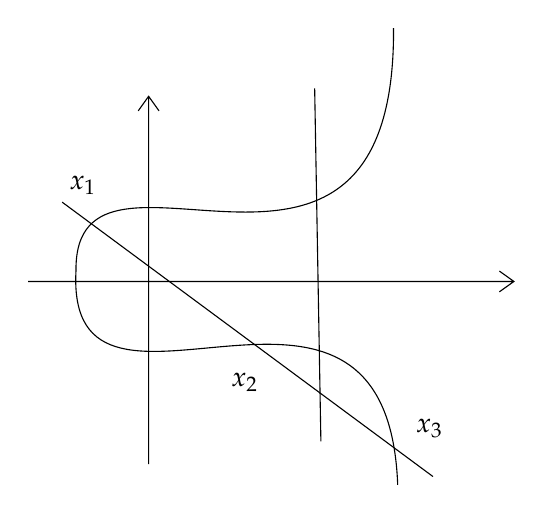
\begin{tikzpicture}[x=0.75pt,y=0.75pt,yscale=-1,xscale=1]
%uncomment if require: \path (0,300); %set diagram left start at 0, and has height of 300

\draw  (240.65,150.2) -- (474.65,150.2)(298.65,61) -- (298.65,238.2) (467.65,145.2) -- (474.65,150.2) -- (467.65,155.2) (293.65,68) -- (298.65,61) -- (303.65,68)  ;
\draw    (263.65,145.2) .. controls (262.65,64.2) and (417.65,189.2) .. (416.65,28.2) ;


\draw    (263.65,145.2) .. controls (258.65,240.2) and (413.65,112.2) .. (418.65,248.2) ;


\draw    (378.65,57.2) -- (381.65,227.2) ;


\draw    (257,112) -- (435.65,244.2) ;



\draw (267,104) node   {$x_{1}$};
\draw (345,199) node   {$x_{2}$};
\draw (434,221) node   {$x_{3}$};


\end{tikzpicture}

\end{center}
These are exactly the intersection points (with multiplicity for tangents) of $C\cap \affn^2_K\subset \affn^2_K$ with the line $f=0$.

Suppose
$\div(f)=x_1+x_2+x_3-3\infty$, $\Lrta (x_1-\infty)+(x_2-\infty)+(x_3-\infty)=0$ in $\pic^\circ (C)$

$\Llrta x_1+x_2+x_3=0$ in $\{\text{closed points}\}$

Suppose $\beta=0$, $\Lrta \div(f)=x_1+x_2-2\infty$ $\Llrta x_1-\infty+x_2-\infty=0$, $\Llrta x_1+_Cx_2=0$, $\Llrta X_2=-x_1$ in $\{\text{Closed points}\}$.

If $x_1=(u_1,v_1)$ is a point on $C$, then $-x_1=(u_1,-v_1)$ is the inverse.

To compute $x_1+_C x_2$:

$(1a)$: if $x_1\neq x_2$, draw the unique line $L\subset \affn^2_K$ joining  $x_1,x_2$ say $L: f=0$.

$(1a')$ if $L$ is not vertical, let $x_3$
 be the third  intersection point $\div(f)=x_1+x_2+x_3-3\infty$. Then $x_1+x_2$ is the symmetric with $x_3$ with $x$-axis.

 $(1a'')$ if $L$ is vertical, $\Lrta x_1+x_2=0$

$(2a)$ $x_1=x_2$, let $L$ be the tangent line to $C$ at $x_1$, 

$(2a')$ if $L$ is not vertical, then $\div(f)=2x_1+x_3-3\infty$ for some $x-3$ and $2x_1=-x_3$

$(2a'')$
 if $L$ is vertical, then $2x_1=0$.

\begin{rmk}\ 
\begin{enumerate}[label=(\arabic*)]
\item One can check directly that this geometric picture gives an Abelian group law on the set of closed points. Associativity is a famous theorem of euclidean geometry.
\item Elliptic curve cryptography uses this group structure. Having cases leading to ``timing attacks''; often models of elliptic curves are used to avoid this, where all operation are carefully designed to take the same amount of time.
\item Elliptic curves (surprisingly) important in modern arithmetic. (Silverman, the arithmetic of elliptic curves)
\end{enumerate}
\end{rmk}
\section{Riemann hypothesis over finite fields*}
\subsection{May 29th-B: The Riemann hypothesis for curves over finite fields.}

\underline{History:} A.Weil 1940s Great motivating problems for algebraic geometry from 1940s on, including generalizations
(Weil conjectures) as motivating Grothendieck.

Classical Riemann hypothesis
$$
\zeta(s)=\sum_{n=1}^\infty \frac{1}{n^s}
$$
is defined over the region $Re(s)>1$. Riemann showed this function has an analytic continuation to $\cplx$ with a simple pole at $s=1$. This showed $\zeta(-2k)=0$ for $k\geq 1$ integers. He conjectured all other zeros lies on the line of $Re(s)=\frac{1}{2}$.

$$\Llrta\sum_{p\leq x, p\text{ prime}}1=\int^x_2\frac{dt}{\log(t)}+\calo(\sqrt{x}(\log(x)^2))$$


\underline{Question}: Given a finite field $\bbf_q$  with $q$ elements and $C/\bbf_q$ curve. is there an $\bbf_q$-rational point ($\bbf_q$-valued point)? How many are there?

(Note: if $C\inj \proj^n_{\bbf_q}$ then $|C(\bbf_q)|\leq |\proj^n_{\bbf_q}(\bbf_q)|$ is finite, where the later equals
$$
\frac{q^{n+1}-1}{q-1}.
$$
\begin{ex}\ 
\begin{enumerate}[label=(\arabic*)]
\item
Fix $k\geq 2$, $x^k+y^k=z^k$? $x,y,z\in \bbf_q$ not all zero.
 We will se that there are many situations if $p$ is large enough.
 \item $a,b\in \bbf_q$, 
 $$
 \left|\{(x,y)\in \bbf_q^2\mid y^2=x^3+ax+b\}\right|?
 $$
We can find solution by taking any $x\in \bbf_q$ and computing $x^3+ax+b\in\bbf_q$ and asking if it is a square or not in $\bbf_q$. If $q$ is odd, there are
$$
1+\frac{q-1}{2}=\frac{q+1}{2}
$$
squares in $\bbf_1$
$$
\left\{
\begin{aligned}
& \bbf_q^\times\lrta\bbf_q^\times\\
& x\longmapsto x^2
\end{aligned}\right.
$$
has kernel $\{\pm 1\}$ so $|Im|=\frac{q-1}{2}$. One guesses that there is about half chance that $x^3+ax+b$ is a square, so altogether we might expect $\sim 2\cdot \frac{q}{2}=q$ solutions.

\begin{thm}
(Hasse-Weil bound): $\bbf_q$ finite field $C/\bbf_q$ non-singular projective curve. Let $g\geq 0$ be its genus. Then $$\left||C(\bbf_q)|-(q+1)\right|\leq 2g \sqrt{q}$$
\end{thm}

N.B. 
\begin{enumerate}
\item 
$C=\proj^1_{\bbf_q}$, $g=0$
$$
\left||C(\bbf_q)|-(q+1)\right|\leq 0
$$
$$
\Lrta |\proj^1(\bbf_q)|=(q+1)
$$
\item In fact,  Weil proved there exist $\alpha_1,...,\alpha_{2g}$ in $\cplx, |\alpha_i|=\sqrt{q}$ such that for any $\nu\geq 1$
$$
|C(\bbf_{q^\nu})|=q^\nu+1-\sum_{i=1}^{2g}\alpha_i^\nu
$$
$$
\Lrta ||C(\bbf_{q^\nu})|-(q^\nu+1)|\leq 2g \sqrt{q}.
$$
In fact, from earlier work of Hasse, Artin. Schmidt...such a formula was  knowen except that $|\alpha_i|=\sqrt{q}$, the $\alpha_i$ being zeros of a certain polynomial analogue of the zeta function. then $|\alpha_i|=\sqrt{q}$ plays the role of $Re(s)=1/2$
\item Higher dimensional version were conjectured by Weil (1948) proved by Dwark, Grothendieck for the counting formula. and especially R-H by Deligne. For reference see the appendix in Hartshorne or a monograph by James Milne on his webpage.
\end{enumerate}
\end{enumerate}
\end{ex}
We will prove the weaker-looking (though equivalent) statement 
\begin{thm}
(Stepanov 1969 Bombieri 1973)

$C/\bbf_q$ nonsingular projective $q=p^{2\alpha}$, where $p$ prime, $\alpha\geq 1$. If $q> (g+1)^4$, then 
$$
C(\bbf_q)\leq q+1+(2g+2)\sqrt{q}
$$
\end{thm}

\underline{Key idea}

Recall $\bbf_q\subset \overline{\bbf}_q$ is the characterized as $\{x\in \overline{\bbf_q}|x^q=x\}$, which is the fixed point of the power morphism $\varphi_q:\overline{\bbf}_q\lrta\overline{\bbf}_q:x\longmapsto x^q$

Give $C/\bbf_q$, there is a Frobenius automorphism
$$
\begin{aligned}
\varphi_q:&C\lrta C\\
& (x_i)\longmapsto (x_i^q)
\end{aligned}
$$
Intuitively: $C$ is given as solution set of polynomial $f_i(x_1,...,x_m)$ where $f_i\in\bbf_q[X_1,...,X_m]$, then
$$
f_i(X_1^q,..,X_m^q)=f_i(X_1,..,X_m)^q
$$
so if $(x_1,...,x_m)$ are solution then so of $(x_1^q,...,x_m^q)$


Rigorously, the above gives a well-defined 
$$
\varphi_q:\spec(A)\lrta \spec (A)\\
$$
where $A=\bbf_q[X_1,...,X_m]/(I)$ which satisfies the glueing.

Then
$$
C(\bbf_q)\cong \{x\in C(\overline{\bbf}_q|\varphi_q(x)=x\}
$$

\underline{Ex}
$f(x,y)=0$, $x,y$ is a solution in $\bbf_q^2$ $\Llrta $ it is a solution in $\overline{\bbf}_q^2$ and $(x,y)^q=(x^q,y^q)=(x,y)$

\underline{Idea of Stepanov}
Suppose we have 
$$
n\geq 1, m\geq 1 \text{ and } 0\neq f\in \overline{\bbf}_q(C)
$$
such that 
\begin{enumerate}
\item $f$ has at most $n$ poles with multiplicity
\item every $x\in C(\bbf_q)$ is a zero of $f$ with multiplicity $\geq m$. Tenn $\deg(\div(f))=0$ implies 
$$
m|C(\bbf_q)|\leq n
$$
$$
\Llrta |C(\bbf_q)|\leq \frac{n}{m}.
$$
Such ideas exists also in transcendence theory from Thue's time $\sim$ 1910s cf. D. Masser ``Auxiliary polynomials in number theory''.
\end{enumerate}
\begin{proof}[Proof of Stepanov's theorem, following Bombieri]
Let $x_0\in C(\bbf_q)$ fixed. (If $x_0$ does not exist, the result is true).
Let $D_n=nx_0\in \Div(C)$ and we will find  a suitable auxiliary function $f$ in $\Gamma(C,\call(D_n))$ for $n$ large enough. Such  a function certainly has poler divisor of degree $\leq n$. We will find $f=g^m$, with $g$ vanishing at all $x\in C(\bbf_q)-\{x_0\}$
$$
\Lrta m(|C(\bbf_q)|-1)\leq n
$$
$$
|C(\bbf_q|\leq 1+\frac{n}{m}
$$
They key is to do this with $n$ as small as posible and $m$ as large as possible.
\end{proof}

\subsection{June 1st:}
\underline{Goal:} $C/\bbf_q$ nonsingular projective curve with genus $g\geq 0$.
$$
||C(\bbf_q)|-(q+1|\leq 2g \sqrt{q}.
$$
\begin{thm}
[Stepanov]
$$
|C(\bbf_q)|\leq q+1+(2g+1)\sqrt{q}
$$
if 
$$
\left\{\begin{aligned}
&q> (g+1)^4\\
&q \text{ is a square}
\end{aligned}\right.
$$
\end{thm}

Idea. constuct $f\in \bbf_q(C)$ non-zerp, wtih at most a pole of order $n\geq 1$ at some fixed  $x_0\in C(\bbf_q)$, and with zeros of multiplicity $\geq m$ at all $x\ni C(\bbf_q)-\{x_0\}$
$$
\Lrta |C(\bbf_q|\leq 1+\frac{n}{m}.
$$
Fix $x_0$ (if $C(\bbf_q)=\emptyset$, then theorem holds)

$V_n=f(\Gamma(C\times \overline{\bbf}_q,\call(D_n)))$, $V_n$ is a finite  dimensional $\bbf_q$-vector space, where $D_n=n x_0$.

We search for $f$ of the form 
$$
0\neq \sum_i g_i^{p^{\mu}}\cdot (f_i\circ \varphi_q)=f
$$
where $g_i\in V_n$, $f_i\in V_m$ for suitable $n,m,\mu$, we want
$$
\delta f=\sum_i g_i^{p^\mu} f_i
=0$$
in $\overline{\bbf}_q(C)$. If this is the case then $f(x)=0$ for all $x\in C(\bbf_q)-\{x_0\}$ because  for such an $x$ 
$$
\begin{aligned}
f(x)&=\sum_i g_i(x)^{p^\mu} f_i (\varphi_q(x))\\
&=\sum_i g_i(x)^{p^\mu}f_i(x)\\
&=(\delta f)(x)=0.
\end{aligned}
$$
If $p^\mu|q$ then $f$ is also a $p^\mu$-th power in $\overline{\bbf}_q(C)^x$:
$$
\begin{aligned}
f&= \sum_i g_i^{p^\mu} f_i \circ \varphi_q\\
&= \sum_i g_i^{p^\mu} \tilde{f}_i^{q}\\
&=\sum_i (g_i \tilde{f}_i^{q/p^{\mu}})^{p^{\mu}}=\left(\sum_i g_i \tilde{f}_i^{q/p^\mu}\right)^{p^\mu}.
\end{aligned}
$$
So the order of vanishing of $f$ at $x\in C(\bbf_q)-\{x_0\}$ is $\geq p^\mu$.
(Why is $f_i\circ \varphi_q$ a $q$-th power?)

\underline{Affine case}:
$$
f_i\in\overline{\bbf}_q[X_1,..,X_m]
$$
$$
\begin{aligned}
f_i\circ \varphi_q&=f_i(X_1^q,...,X_m^q)\\
& =\sum_{I}\alpha_I X_1^{ q i_1}\cdots X_m^{q i_m}\\
&= \left(\sum_I \beta_I X_i^{i_1}\cdots X_m^{i_m}\right)^q
\end{aligned}
$$
where $\beta_I^q=\alpha_I$.

$
f=\sum_i g_i^{p^\mu}(f_i\circ \varphi_q)
$, $\delta f$ is linear in $g_i,f_i$ but it could be that  whenever we get $\delta f=0$. we also have $f=0$.

\underline{Define}:
$$
V_n^{(\mu)=\{g^{p^\mu}|g\in V_n\}}.
$$ $V_n^{(\mu)}$ is an $\overline{\bbf}_q$-vector subspace of $V_{n p^\mu}$, $\dim V_n^{(\mu)}=\dim V)n=\ell(D_n)$.
$$
\tilde{V}_m=\{f\circ \varphi_q|f\in V_m\}
$$
is also an $\overline{\bbf}_q$-space, and 
$$
\tilde{V}_m\subset V_{q m},
$$
$$
\dim (\tilde{V}_m)=\dim(V_m)=\ell(D_m).
$$

\begin{lemma}
Assume $m\geq 1, n\geq 1,\mu\geq 1$, and
$$
np^\mu< q.
$$
Then the multiplication map
$$
\left\{
\begin{aligned}
&V_n^{(\mu)}\otimes_{\overline{\bbf}_q}\tilde{V}_m\lrta \overline{\bbf}_q(C)\\
&g^{p^\mu}\otimes(f\circ \varphi_q)\longmapsto g^{p^\mu}(f\circ \varphi_q)
\end{aligned}
\right.
$$
is surjective.
$\Lrta $ the image has dimension $\ell(D_m)\ell(D_n)$.
\end{lemma}
\begin{proof}
Let $d=\ell(D)_m$, let 
$(f_1,...,f_d)$ be a basis of $V_m$, chosen so that 
$$
V_{X_0}(f_i)< V_{X_0}(f_{i+1})
$$
for $1\leq i\leq d-1$ such a bsisi exists because $\dim (V_{i+1}/V_i)\leq 1$ since if $f_1,f_2\in V_{i+1}$ have pole of order $i+1$, then some $\alpha f_1+\beta f_2$ has pole of order $\leq 1$.

For example, $\proj^1$,  $x_0=\infty$ $V_\infty(f)=-\deg(f)$ for $f$ polynomial. $f_1=X^d$, $-d$, $f_2=X^{d_1}, -d+1$


Any $f \in V_n^{(\mu)\otimes \tilde{V}_m}$ has an expansion
$$
\sum_{i=1}^{d}g_i^{p^\mu}\cdot(f_i\circ \varphi_q)
$$
for some $f_i\in V_m$ the tensor product is spanned by 
$$
\begin{aligned}
&\sum_i \tilde{g}_j^{p^\mu}\otimes\left((\sum_i \alpha_{ij}f_i)\circ \varphi_q\right)\\
&= \sum_i (\sum_j \alpha_{ij}\tilde{g}_{j}^{p^\mu})\otimes (f_i\circ \varphi_q)\\
g_i---(\sum_i \beta_{ij}\tilde{g}_j)^{p^\mu}
\end{aligned}
$$
Assume 
$$
\sum_{i=1}^d g_i^{p^\mu}(f_i\circ \varphi_1)=0,
$$
we will check that $f_i=0$ for all $i$, so that $f=0$. Assume
 some $g_i\neq 0$, say $g_1=\cdots=g_{k-1}=0$ and $g_k\neq 0$
  so
  $$
V_{x_0}(g_k^{p^\mu}f_k\circ \varphi_q)
=V_{x_0}\left(\sum_{i\geq k} g_i^{p^\mu}(f_i\circ \varphi_q)\right).  $$
The $LHS=p^\mu V_{x_0}(g_k)+qV_{x_0}(f_k)$, while the
$$
\begin{aligned}
RHS&\geq \min_{i\ >k}V_{x_0}(g_i^{p^\mu}f_i\circ \varphi_q)\\
&\geq -np^\mu+qV_{x_0}(f_i).
\end{aligned}
$$ 
So we have
$$
p^\mu V_{x_0}(f_k)\geq -n p^\mu+ q(V_{x_0}(f_i)-V_{x_0}(f_k))\geq -n p^\mu+q\geq 1\text{ by assumption}
$$
where $V_{x_0}(f_i)-V_{x_0}(f_k)\geq 1$.
Hence, $g_k$ is defined at $x_0$ (in fact vanishes at $x_0$) so $g_k\in \Gamma(C\times \overline{\bbf}_q,\calo_C)$ is constant, so equal to $0$. Contradiction!
\end{proof}

Let $W_{n,m}$ be the image  of this map. The lemma shows that if $n p^\mu<q$, the map 
$$
\delta:\left\{
\begin{aligned}
W_{n,m}&\lrta \overline{\bbf}_q(C)\\
\sum_{i=1}^d
g_i^{p^\mu}(f_i\circ \varphi_q)&
\longmapsto \sum_{i=1}^d g_i^{p^\mu}f_i
\end{aligned}\right.
$$
is a well-defined $\overline{\bbf}_q$-linear map. 
$$
\dim \ker(\delta)=\dim(W_{n,m})-\dim Im(\delta)=\ell(D_m)\ell(D_n)--\dim Im(\delta).
$$
But $Im_{\delta}\subset V_{np^\mu+m}$ so 
$$
\dim \ker(\delta)\geq \ell(D_n)\ell(D_m)-\ell(D_{np^\mu+m}).
$$
Conclusion:
if $n,m,\mu\geq 1$ and 
$p^\mu|q$, $np^\mu<q$ $\ell(D_n)\ell)D_m> \ell(D_{p^\mu n+m})$ then 
$$
|C(\bbf_q)|\leq 1+\frac{p^\mu n+ m q}{p^{\mu}}=1+n+\frac{mq}{p^\mu}
$$
(need $n,m$ as small as possible $\mu$ as large as possible)

R-R:
$$
\ell(D)n
-\ell(K_C-D_n)=n+1-g
$$
so $\ell(D_n)\geq n+1 -g$ $\ell(D_m)\geq m+1 -g$. and $\ell(D_{n p^\mu +m})=np^\mu+m+1-g$ if $np^\mu +m> 2g-2$. So we  get  non-trivial kernel if 
$$
(n+1-g)(m+1-g)> np^\mu+m+1-g
$$
and 
$$
np^\mu < q.
$$
Thinking that $g$ is fixed and small, we guess that we can take $m\sim p^\mu$, the bound becomes $1+n+q$. the bound becomes $1+n+q$. 

Looking at the ``lower-order terms'', we see that the best possible choice is $m\sim n\sim p^\mu$. Then the best $\mu$ is when  $q=p^{2\mu}$ (so $q$ is a square) and $n$ just  a bit smaller. More precisely, the values below work
$$
q=p^{2\mu}
$$
$$
m=p^\mu+2g=\sqrt{q}+2g
$$
$$
n=\left\lfloor \frac{g}{g+1}p^\mu\right\rfloor +g+1
$$

and then
$$
|C(\bbf_q)|\leq 1+\frac{m q}{p^\mu}+n =1+q+2g p^\mu +g+1+ \left\lfloor \frac{g}{g+1}p^\mu\right\rfloor< 1+q+(2g+1)\sqrt{q}
$$
if $q > (g+1)^4$.  How to get the lower bound ? To get a lower bound 
$$
|C(\bbf_q)|\geq q- C\sqrt{q}
$$
for some $C\geq 1$, Stepanov(-Bambieri) use a trick from Galois theory.

\begin{ex}
Suppose $C:Y^d=g(X)$, $d\geq 2$ and $g$  is square free. 
Idea: find $C_\alpha$ auxiliary curve $\alpha\in A$, s.t. 
$$
\sum_{\alpha\in A}|C_\alpha(\bbf_q)|=(simple)=|A|q
$$
and 
$$
|C_\alpha(\bbf_q|\leq q+ C\sqrt{q}
$$
then the sum of $C_\alpha(\bbf_q)$, $\alpha\neq 1$, cannot compensate a too small value of $|C_1(\bbf_q)|$.
\end{ex}

Hence $A=\bbf^\times_q/(\bbf^\times_q)^d$ is a cyclic group of order $d$ (since $d|q-1$). Let $A\subset \bbf^\times_q$ be a set of  representative of $\tilde{A}$, with $1\in A$.
$C_\alpha:\alpha Y^d=g(x)$, one can check that $C_\alpha$ is still of genus $g$. So Stepanov derived 
$\Lrta |C_\alpha(\bbf_q)|\leq q+1+C\sqrt{q}$ where $C$ is independent of $\alpha$.  But
 $$
 \begin{aligned}
 \sum_{\alpha\in A}|C_\alpha(\bbf_q)|&=\sum_{\alpha\in A}\sum_{x,y\in \bbf_q, y^d=\alpha^{-1}g(x)}1\\
 &=\sum_{x\in \bbf_q}\sum_{g(x)=\alpha y^d}1\\
 &=(\text{ at most $\deg g$ zeros of $g$})+ d(q-\# \text{ of zeros of $g$} )\\
 &= dq +O(\deg (g)).
 \end{aligned}
 $$
 Last Step: from ``
  $$
  |C(\bbf_{q^{2\nu}})|=q^{2\nu}+O(q^\nu)
  $$
  for all $\nu$ large enough.''
  to
  $$
||C(\bbf_{q^\nu})|-(q^\nu+1)|\leq 2g \sqrt{q^\nu}
  $$
We input 
\begin{thm}
[Hasse, Artin. Schmidt, 1930s]. There are $\alpha_1,...,\alpha_{2g}$ in $\cplx$ such that
 $$|C(\bbf_{q^\nu})|=q^\nu+1-\sum^{2g}_{i=1}\alpha_i^\nu, \nu \geq 1$$ 
 and $q/\alpha_i$ is one of the $\alpha_j$'s
\end{thm}
and the proof uses Riemann-Roch again.

Combining the above arguments, we get
$\exists C\geq 0$, $|\sum_{i=1}^{2g}\alpha_i^{2\nu}|\leq C q^\nu$ for all $\nu \geq \nu_0$ in fact $\nu \geq 0$ by increasing $C$. 
\begin{lemma}
Suppose $\beta_1,...,\beta_r\in \cplx$, satisfy 
$$
|\sum_i^\nu \beta_i^r|\leq C B^\nu
$$
for $\nu \geq 0$. Then $|\beta_i|\leq B$. 
\end{lemma}
\begin{proof}[Proof of Lemma]
$$
\begin{aligned}
f(z)&=\sum_{\nu \geq 0}\left(\sum_{i=1}^r\beta_i^\nu\right)z^\nu\\
&=\sum_{i=1}^r\sum_{\nu\geq 0}(\beta_i z)^\nu\\
&=\sum^r_{i=1}\frac{1}{1-\beta_i z}
\end{aligned}
$$
has poles at each $\frac{1}{\beta_i}$.

Hypothesis $\Lrta$ $f$ converges for $|z|<\frac{1}{|B|}$ so we have
$$
\frac{1}{|\beta_i|}\geq \frac{1}{|B|}
$$
$\Lrta |\beta_i|\leq |B|$ for all $i$.
\end{proof}

\underline{Conclusion}
$\beta_i=\alpha_i^2$, $B=q$

$\Lrta |\alpha_i^2|\leq q$, $\Lrta |\alpha_i|\leq \sqrt{q}$

$\Lrta ||C(\bbf_q|-(q+1)|\leq 2g\sqrt{q}$ but also 
$\left|\frac{q}{\alpha_i}\right|\leq \sqrt{q}\Lrta |\alpha_i|\geq \sqrt{q}$. These give us the final result
$$
|\alpha_i|=\sqrt{q}
$$
which is equivalent to the Riemann-Hypothesis on finite field.


Consider $C/\bbf_q$ elliptic curve

\underline{Step 1}. $Z(T)=\exp\left(\sum_{\nu\geq 1}\frac{|C(\bbf_{q^\nu})|}{\nu} T^\nu\right)$. We have
 $$
 Z(T)=\prod_{x\text{ closed point of }C}(1- T^{\deg(x)})^{-1}
 $$
 where $\deg(x:=[\kappa(x):\bbf_q])$

 \underline{Step 2}:
 $$
 Z(T)=\sum_{D\geq 0\text{, div of } C} T^{\deg(D)}=1+\sum_{d\geq }T^d \sum_{\deg(D)=d, D\geq 0} 1
 $$
\end{document}

